%%%%%%%%%%%%%%%%%%%%%%%%%%%%%%%%%%%%%%%%%
% Uppsala University Assignment Title Page 
% LaTeX Template
% Version 1.0 (27/12/12)
%
% This template has been downloaded from:
% http://www.LaTeXTemplates.com
%
% Original author:
% WikiBooks (http://en.wikibooks.org/wiki/LaTeX/Title_Creation)
% Modified by Elsa Slattegard to fit Uppsala university
% License:
% CC BY-NC-SA 3.0 (http://creativecommons.org/licenses/by-nc-sa/3.0/)

%\title{Title page with logo}
%----------------------------------------------------------------------------------------
%	PACKAGES AND OTHER DOCUMENT CONFIGURATIONS
%----------------------------------------------------------------------------------------

\documentclass[12pt]{article}
\usepackage[margin=1in]{geometry} 
\usepackage{amsmath,amsthm,amssymb,scrextend}
\usepackage{fancyhdr}
\pagestyle{fancy}
\DeclareMathOperator{\rng}{Rng}
\DeclareMathOperator{\dom}{Dom}
\newcommand{\R}{\mathbb R}
\newcommand{\cont}{\subseteq}
\newcommand{\N}{\mathbb N}
\newcommand{\Z}{\mathbb Z}
\usepackage{tikz}
\usepackage{pgfplots}
\usepackage{amsmath}
\usepackage[mathscr]{euscript}
\let\euscr\mathscr \let\mathscr\relax
\usepackage[scr]{rsfso}
\usepackage{amsthm}
\usepackage{amssymb}
\usepackage{multicol}
\usepackage[colorlinks=true, pdfstartview=FitV, linkcolor=blue,
citecolor=blue, urlcolor=blue]{hyperref}
\usepackage[spanish]{babel}
\usetikzlibrary{babel,positioning,arrows.meta}
\usepackage[utf8]{inputenc}
\newtheorem*{defi}{Definición}
\newtheorem*{Tem}{Teorema}
\spanishdecimal{.}

\begin{document}

\begin{titlepage}

\newcommand{\HRule}{\rule{\linewidth}{0.5mm}} % Defines a new command for the horizontal lines, change thickness here

\center % Center everything on the page
 
%----------------------------------------------------------------------------------------
%	HEADING SECTIONS
%----------------------------------------------------------------------------------------

\textsc{\LARGE Universidad Nacional Autónoma de México}\\[1.5cm] % Name of your university/college
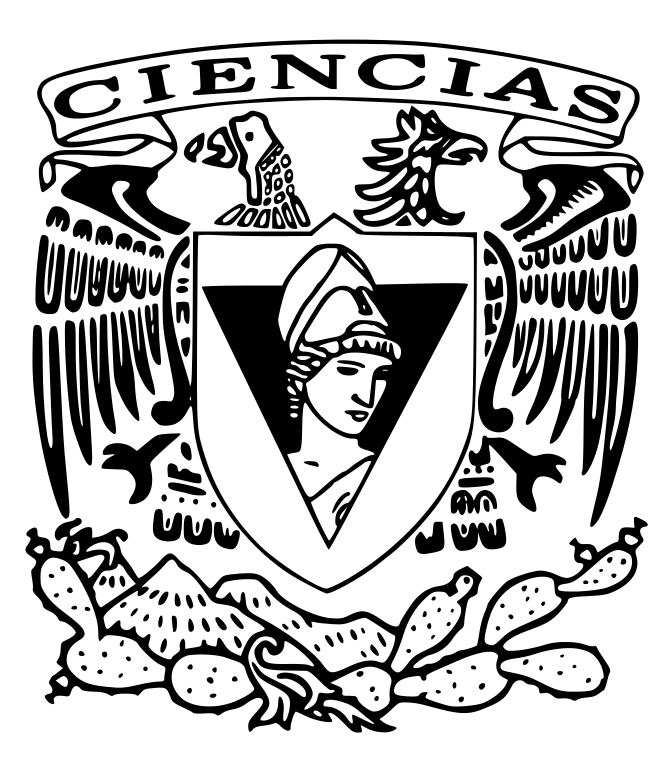
\includegraphics[scale=.2]{images/escudo.png}\\[1cm] % Include a department/university logo - this will require the graphicx package
\textsc{\Large  Heuristicas de Optimización Combinatoria}\\[0.5cm] % Major heading such as course name
\textsc{\large Reporte Proyecto 1}\\[0.5cm] % Minor heading such as course title

%----------------------------------------------------------------------------------------
%	TITLE SECTION
%----------------------------------------------------------------------------------------

\HRule \\[0.4cm]
{ \huge \bfseries Implementación de Recocido Simulado basada en Aceptación por Umbrales para resolver instancias del Problema del Agente Viajero (TSP)}\\[0.4cm] % Title of your document
\HRule \\[1.5cm]
 
%----------------------------------------------------------------------------------------
%	AUTHOR SECTION
%----------------------------------------------------------------------------------------

\begin{minipage}{0.4\textwidth}
\begin{flushleft} \large
\emph{Nombres:}\\
Ricardo Flores Mata 422127808\\ % Your name
\end{flushleft}

\end{minipage}\\[2cm]

% If you don't want a supervisor, uncomment the two lines below and remove the section above
%\Large \emph{Author:}\\
%John \textsc{Smith}\\[3cm] % Your name

%----------------------------------------------------------------------------------------
%	DATE SECTION
%----------------------------------------------------------------------------------------

{\large \today}\\[2cm] % Date, change the \today to a set date if you want to be precise

\vfill % Fill the rest of the page with whitespace

\end{titlepage}

\clearpage

\section{Introducción}
\label{sec:introduccion}

El presente proyecto aborda el Problema del Agente Viajero
(\textit{Traveling Salesman Problem}, TSP) mediante una estrategia de
Recocido Simulado basada en la heurística de Aceptación por Umbrales
(\textit{Threshold Accepting}). El objetivo principal consiste en diseñar,
implementar y evaluar un sistema capaz de encontrar soluciones de buena
calidad para distintas instancias del problema, utilizando un procedimiento
heurístico que permita explorar el espacio de soluciones sin limitar la
búsqueda únicamente a movimientos que mejoren de manera inmediata la
solución actual, mediante la búsqueda local de vecindarios.
\\\\
El sistema fue implementado en Java y se diseñó separando los componentes
correspondientes a la representación del problema, la función objetivo, la
generación de soluciones vecinas, el acceso a los datos y la propia
heurística. Las ciudades y las conexiones disponibles entre ellas se
obtienen de una base de datos, con soporte para SQLite y PostgreSQL,
mientras que cada instancia del TSP se especifica mediante un archivo que
contiene los identificadores de las ciudades que participan en el problema.
La función objetivo utilizada permite evaluar las permutaciones generadas y
penaliza aquellas soluciones que requieren conexiones inexistentes en la
base de datos.
\\\\
Además de una ejecución normal con parámetros previamente establecidos, se
desarrolló un entorno experimental para explorar automáticamente diferentes
configuraciones de la heurística. Dicho entorno permite variar parámetros
como el factor de enfriamiento, la temperatura mínima, el tamaño de los
lotes y el número máximo de intentos, así como calcular una temperatura
inicial a partir de una tasa objetivo de aceptación. Cada configuración es
evaluada utilizando múltiples semillas pseudoaleatorias con el propósito de
analizar no solamente la mejor solución obtenida, sino también la
consistencia de su desempeño.
\\\\
La evaluación experimental se realizó principalmente sobre dos instancias,
una formada por 40 ciudades y otra por 150 ciudades. Durante
aproximadamente una semana y media se llevaron a cabo ejecuciones
experimentales para estudiar el comportamiento de la heurística, identificar
regiones adecuadas del espacio de parámetros y comparar el desempeño del
sistema conforme aumenta el tamaño de la instancia. A partir de estas
ejecuciones se generaron reportes que incluyen los costos obtenidos, número
de vecinos generados y aceptados, niveles de temperatura, tiempos de
ejecución y evolución de las mejores configuraciones encontradas.
\\\\
En este reporte se presenta primero la formulación del Problema del Agente
Viajero y posteriormente se describe la heurística de Aceptación por
Umbrales utilizada para resolverlo. Después se expone el diseño y la
implementación del sistema, incluyendo la representación de las soluciones,
el cálculo de costos, el vecindario, el manejo de semillas y el entorno de
búsqueda experimental de parámetros. Finalmente, se presentan y analizan
los resultados obtenidos para las instancias de 40 y 150 ciudades, con el
apoyo de tablas y gráficas que permiten estudiar el comportamiento y el
desempeño de la implementación.

\clearpage

\section{Problema del Agente Viajero}
\label{sec:tsp}

El Problema del Agente Viajero
(\textit{Traveling Salesman Problem}, TSP) es uno de los problemas más
conocidos dentro de la optimización combinatoria. En su formulación clásica,
se dispone de un conjunto de ciudades y de un costo asociado al
desplazamiento entre cada par de ellas. El objetivo consiste en encontrar un
recorrido de costo mínimo que visite cada ciudad exactamente una vez y
regrese finalmente a la ciudad de origen \cite{lawler1985tsp}.
\\\\
El problema puede modelarse mediante una gráfica ponderada
\[
    G=(V,E),
\]
donde \(V\) representa el conjunto de ciudades y \(E\) el conjunto de
conexiones existentes entre ellas. A cada arista
\((v_i,v_j)\in E\) se le asocia un peso
\[
    c_{ij}\geq 0,
\]
que representa el costo o distancia de viajar desde la ciudad \(v_i\) hasta
la ciudad \(v_j\).
\\\\
Si la instancia contiene \(n\) ciudades, una solución puede representarse
mediante una permutación
\[
    \pi =
    \left(
        \pi_1,\pi_2,\ldots,\pi_n
    \right),
\]
donde cada elemento de \(V\) aparece exactamente una vez. En la formulación
clásica del TSP, el costo del recorrido correspondiente a dicha permutación
es
\[
    f(\pi)
    =
    \sum_{i=1}^{n-1}
    c_{\pi_i,\pi_{i+1}}
    +
    c_{\pi_n,\pi_1}.
\]
El último término representa el regreso desde la última ciudad hasta la
primera, de manera que la solución forma un ciclo hamiltoniano.

\subsection{Complejidad del problema}

El TSP es un problema computacionalmente difícil. Su versión de
optimización pertenece a la clase de problemas NP-duros, mientras que su
versión de decisión se encuentra entre los problemas NP-completos
\cite{garey1979computers}. Esto implica que no se conoce un algoritmo que
encuentre la solución óptima para todas las instancias en tiempo polinomial.
\\\\
Incluso utilizando únicamente la representación por permutaciones, el
espacio de búsqueda crece factorialmente. Para \(n\) ciudades existen, en
principio,
\[
    n!
\]
ordenamientos posibles. 
\\\\
Si se consideran equivalencias por rotación y por
sentido del recorrido en el TSP simétrico clásico, el número puede reducirse,
pero su crecimiento continúa siendo factorial.

Por ejemplo,
\[
    40!
    \approx
    8.16\times 10^{47},
\]

mientras que para una instancia de 150 ciudades,
\[
    150!
    \approx
    5.71\times 10^{262}.
\]
Estas cantidades hacen inviable una exploración exhaustiva del espacio de
soluciones para las instancias consideradas en este proyecto. Por ello se
recurre a una heurística que permita explorar solamente una fracción del
espacio de búsqueda con el objetivo de obtener soluciones de buena calidad
en un tiempo razonable.

\subsection{Representación utilizada en el proyecto}

En la implementación desarrollada, una instancia se define a partir de un
conjunto de identificadores de ciudades almacenadas previamente en una base
de datos. Por ejemplo, un archivo de entrada puede contener
\begin{verbatim}
1,7,15,28,31
\end{verbatim}
indicando que únicamente esas ciudades formarán parte de la instancia que
deberá resolver el programa.
\\\\
Una solución se representa nuevamente mediante una permutación de las
ciudades. Sin embargo, internamente el sistema no trabaja directamente con
los identificadores de la base de datos, sino con índices consecutivos
\[
    0,1,\ldots,n-1.
\]
Por ejemplo, para una instancia cuyos identificadores reales sean
\[
    (7,25,81,103),
\]
la representación interna utiliza la correspondencia
\[
\begin{aligned}
    0 &\longleftrightarrow 7,\\
    1 &\longleftrightarrow 25,\\
    2 &\longleftrightarrow 81,\\
    3 &\longleftrightarrow 103.
\end{aligned}
\]
Esta transformación permite utilizar arreglos y matrices para consultar los
costos entre ciudades de manera eficiente, independientemente de los
identificadores originales almacenados en la base de datos.

\subsection{Particularidades de las instancias utilizadas \\ }
\label{subsec:particularidades-tsp}

La formulación utilizada en este proyecto sigue una variante del TSP
establecida para el sistema. Las ciudades y sus conexiones se representan
mediante una gráfica ponderada
\[
    G=(V,E),
    \qquad
    E\subseteq V\times V,
\]
junto con una función de peso
\[
    w:E\longrightarrow \mathbb{R}^{+},
\]
donde \(V\) es el conjunto de ciudades, \(E\) el conjunto de conexiones
existentes y \(w(u,v)\) representa la distancia correspondiente a una
conexión entre las ciudades \(u\) y \(v\).
\\\\
Una instancia particular del TSP se determina mediante un subconjunto
\[
    S\subseteq V.
\]
Es decir, \(S\) contiene exactamente las ciudades que se desean considerar
en una ejecución del problema. Si
\[
    S=\{v_1,v_2,\ldots,v_k\},
\]
entonces se busca una trayectoria que pase por cada uno de estos \(k\)
vértices.
\\\\
Una característica importante de la gráfica \(G\) es que no necesariamente
es completa. Por lo tanto, pueden existir dos ciudades \(u,v\in S\) para
las cuales la arista \((u,v)\) no pertenezca a \(E\). Para poder trabajar
con cualquier permutación de los elementos de \(S\), se construye
conceptualmente una gráfica completa
\[
    G_S=(V_S,E_S),
\]
donde
\[
    V_S=S
\]
y
\[
    E_S=
    \{(u,v)\mid u,v\in S,\ u\neq v\}.
\]
Sobre esta gráfica se define una función de peso aumentada
\[
    w_S:E_S\longrightarrow\mathbb{R}^{+},
\]
dada por
\[
w_S(u,v)=
\begin{cases}
    w(u,v),
        & \text{si }(u,v)\in E,\\[2mm]
    d(u,v)\,\max{}' d(S),
        & \text{en otro caso}.
\end{cases}
\]
Aquí, \(d(u,v)\) representa la distancia natural entre las ciudades
\(u\) y \(v\), calculada a partir de sus coordenadas geográficas, mientras
que \(\max{}'d(S)\) representa la mayor distancia correspondiente a una
conexión existente entre dos ciudades de \(S\):
\[
    \max{}'d(S)
    =
    \max
    \left\{
        w(u,v)
        \mid
        u,v\in S,\ (u,v)\in E
    \right\}.
\]
De esta manera, cuando una conexión existe en la gráfica original se utiliza
directamente su distancia almacenada. En cambio, cuando la conexión no
existe, se le asigna un peso considerablemente mayor mediante la distancia
natural multiplicada por la distancia máxima de la instancia. Esto permite
que el algoritmo pueda evaluar cualquier permutación de \(S\), pero al mismo
tiempo penaliza aquellas soluciones que utilizan conexiones inexistentes.
\\\\
Dada una instancia \(S\), cualquier permutación
\[
    P=
    v_{\rho(1)},
    v_{\rho(2)},
    \ldots,
    v_{\rho(k)}
\]
de sus elementos constituye una solución en la gráfica completa \(G_S\).
Sin embargo, una solución será \emph{factible} con respecto a la gráfica
original \(G\) si y sólo si todas las conexiones entre elementos
consecutivos existen en \(E\); es decir,
\[
    \left(
        v_{\rho(i-1)},
        v_{\rho(i)}
    \right)
    \in E,
    \qquad
    i=2,\ldots,k.
\]
Si al menos una de estas conexiones no pertenece a \(E\), la solución se
considera no factible.
\\\\
Para comparar las soluciones encontradas se utiliza además un normalizador
\(N(S)\). Para construirlo se consideran las distancias de las conexiones
existentes entre elementos de \(S\), se ordenan de mayor a menor y se toman,
cuando existen suficientes, las \(k-1\) más grandes. Si \(L'\) denota este
conjunto de distancias, entonces
\[
    N(S)
    =
    \sum_{d\in L'} d.
\]
El normalizador permite expresar el costo de las soluciones factibles en una
escala comparable. En particular, una solución factible tendrá una
evaluación entre \(0\) y \(1\), mientras que el uso de la función de peso
aumentada provoca que una solución no factible tenga una evaluación mayor
que \(1\).
\\\\
Finalmente, la función objetivo utilizada en el proyecto es exactamente la
función de costo definida sobre una permutación \(P\) de los elementos de
\(S\):
\[
    \boxed{
    f(P)
    =
    \frac{
        \displaystyle
        \sum_{i=2}^{k}
        w_S
        \left(
            v_{\rho(i-1)},
            v_{\rho(i)}
        \right)
    }{
        N(S)
    }
    }
\]
Por lo tanto, el objetivo del sistema es encontrar una permutación
\(P\) que minimice \(f(P)\).
\\\\
Es importante observar que en esta formulación se consideran únicamente las
\(k-1\) conexiones entre elementos consecutivos de la permutación. No se
agrega una conexión entre el último elemento
\(v_{\rho(k)}\) y el primero \(v_{\rho(1)}\). En consecuencia, el problema
estudiado busca la trayectoria de menor costo que pase por todas las
ciudades de \(S\), en lugar de exigir un ciclo que regrese necesariamente
a la ciudad inicial.

\subsection{Instancias estudiadas}

Para evaluar el comportamiento del sistema se trabajó principalmente con
dos tamaños de instancia:
\[
    n=40
    \qquad\text{y}\qquad
    n=150.
\]
La instancia de 40 ciudades permitió realizar un número elevado de
ejecuciones y estudiar con mayor rapidez el efecto de los parámetros de la
heurística. Posteriormente, la instancia de 150 ciudades permitió analizar
el comportamiento del mismo método sobre un espacio de búsqueda
considerablemente mayor.
\\
Ambas instancias fueron utilizadas tanto para verificar el funcionamiento
del sistema como para realizar la búsqueda experimental de parámetros. Los
resultados obtenidos con ellas se presentan posteriormente en la
Sección~\ref{sec:resultados}.

\section{Aceptación por Umbrales}
\label{sec:aceptacion-umbrales}

Para resolver las instancias del Problema del Agente Viajero descritas en la
sección anterior se utilizó la heurística de \emph{Aceptación por Umbrales}
(\textit{Threshold Accepting}). Esta técnica fue propuesta por Dueck y
Scheuer como una variante del Recocido Simulado, cuya idea general consiste
en permitir temporalmente movimientos que empeoren la solución actual con
el propósito de evitar que la búsqueda quede atrapada prematuramente en un
mínimo local \cite{dueck1990threshold}.
\\\\
Sea
\(\mathcal{S}\) el conjunto de posibles soluciones de una instancia de un
problema de optimización, y sea
\[  f:\mathcal{S}\longrightarrow\mathbb{R}^{+}
\]
su función objetivo, de tal manera que
\[
    0\leq f(s)<\infty
\]
para toda solución \(s\in\mathcal{S}\). \\ Debido a que el problema estudiado
es de minimización, dadas dos soluciones \(s,s'\in\mathcal{S}\), se
considera que \(s\) es mejor que \(s'\) cuando
\[
    f(s)<f(s').
\]
La heurística realiza una búsqueda local sobre este espacio. Si mediante una
operación previamente definida es posible transformar una solución \(s\) en
otra solución \(s'\), ambas se consideran soluciones vecinas. En el caso del
TSP implementado en este proyecto, el vecindario se obtiene mediante el
intercambio de dos posiciones de una permutación, como se explicará con
detalle en la Sección~\ref{sec:implementacion}.

\subsection{Criterio de aceptación}
\label{subsec:criterio-aceptacion}

La característica principal de Aceptación por Umbrales es que una solución
vecina no necesita ser estrictamente mejor que la solución actual para ser
aceptada.
\\\\
Sea \(T\in\mathbb{R}^{+}\) la temperatura actual. Dada una solución
\(s\), se genera aleatoriamente una solución vecina \(s'\). Esta nueva
solución es aceptada si satisface
\[
    \boxed{
        f(s')\leq f(s)+T
    }.
\]
Si la condición se cumple, la solución actual se sustituye por la solución
vecina:
\[
    s\leftarrow s'.
\]
Por lo tanto, toda solución que mejore el costo actual es aceptada, ya que
\[
    f(s')\leq f(s)
    \quad\Longrightarrow\quad
    f(s')\leq f(s)+T.
\]
Sin embargo, también puede aceptarse una solución de mayor costo siempre que
el deterioro no sea mayor que la temperatura:
\[
    f(s)<f(s')\leq f(s)+T.
\]
Esta propiedad permite que la búsqueda abandone mínimos locales y explore
otras regiones del espacio de soluciones.
\\\\
Cuando \(T\) es grande, el intervalo de soluciones que pueden ser aceptadas
es también grande. Conforme \(T\) disminuye, el criterio se vuelve más
restrictivo. Así, durante las primeras etapas de la ejecución se favorece la
exploración del espacio de búsqueda y, en las etapas finales, la heurística
se concentra progresivamente en soluciones de menor costo.

\subsection{Lotes}
\label{subsec:lotes}

El descenso de la temperatura no se realiza después de cada vecino
generado. Para determinar cuándo debe disminuirse se utilizan
\emph{lotes}.
\\\\
Sea
\[
    L\in\mathbb{N}^{+}
\]
el tamaño de lote. Para una temperatura fija \(T\), la heurística genera
vecinos de manera sucesiva hasta obtener \(L\) soluciones aceptadas.
\\\\
Si las soluciones aceptadas durante un lote tienen costos
\[
    f(s_1),f(s_2),\ldots,f(s_L),
\]
se calcula el promedio
\[
    p=
    \frac{1}{L}
    \sum_{i=1}^{L}f(s_i).
\]
El procedimiento devuelve tanto este promedio como la última solución
aceptada. De forma conceptual, el cálculo de un lote puede expresarse como
\[
\begin{array}{l}
    c\leftarrow 0, \qquad r\leftarrow 0,\\[1mm]
    \text{mientras }c<L:\\
    \qquad s'\leftarrow \operatorname{VECINO}(s),\\
    \qquad \text{si }f(s')\leq f(s)+T:\\
    \qquad\qquad s\leftarrow s',\\
    \qquad\qquad c\leftarrow c+1,\\
    \qquad\qquad r\leftarrow r+f(s'),\\[1mm]
    \text{devolver }\left(\dfrac{r}{L},s\right).
\end{array}
\]
Es importante observar que \(L\) representa el número de
\emph{soluciones aceptadas} y no el número de vecinos generados. En
particular, si muchos vecinos son rechazados pueden ser necesarios muchos
más de \(L\) intentos para completar un lote.
\\\\
El procedimiento anterior presenta además un problema práctico: podría no
terminar. Si para una temperatura determinada resulta muy difícil encontrar
vecinos que satisfagan el criterio de aceptación, el número de soluciones
aceptadas podría nunca alcanzar \(L\).
\\\\
Por esta razón se utiliza un número máximo de intentos para completar cada
lote. Dicho límite debe ser considerablemente mayor que \(L\). Si se alcanza
el máximo de intentos sin completar el lote, se considera que éste no pudo
terminarse y la búsqueda de equilibrio para esa temperatura se detiene.

\subsection{Equilibrio térmico y enfriamiento}
\label{subsec:equilibrio}

Para una temperatura fija pueden calcularse varios lotes consecutivos. La
temperatura se mantiene mientras el comportamiento de los costos promedio
indique que la búsqueda continúa avanzando hacia una situación de
equilibrio.
\\\\
Sea \(p\) el promedio del lote anterior y \(q\) el promedio del lote
actual. El esquema utilizado por la heurística es
\[
\begin{array}{l}
    p\leftarrow 0,\\
    \text{mientras }T>\epsilon:\\
    \qquad q\leftarrow\infty,\\
    \qquad \text{mientras }p\leq q:\\
    \qquad\qquad q\leftarrow p,\\
    \qquad\qquad (p,s)\leftarrow
        \operatorname{CALCULALOTE}(T,s),\\
    \qquad T\leftarrow\phi T.
\end{array}
\]
La condición
\[
    p\leq q
\]
permite continuar calculando lotes para una misma temperatura hasta que el
comportamiento de sus promedios indique que se alcanzó el equilibrio
establecido por la heurística.
\\\\
Una vez alcanzado éste, la temperatura se reduce utilizando un factor de
enfriamiento
\[
    0<\phi<1
\]
mediante la expresión
\[
    \boxed{
        T_{\text{nueva}}=\phi T_{\text{actual}}
    }.
\]
El parámetro \(\phi\) determina la rapidez con la que se enfría el sistema.
Un valor muy cercano a \(1\) provoca una disminución lenta de la
temperatura, produciendo una búsqueda más extensa pero también tiempos de
ejecución mayores. Por el contrario, un valor pequeño produce un
enfriamiento rápido y reduce el tiempo de ejecución, aunque puede disminuir
la calidad de las soluciones encontradas.
\\\\
La heurística continúa mientras
\[
    T>\epsilon,
\]
donde \(\epsilon>0\) es un valor suficientemente pequeño que funciona como
un cero virtual para la temperatura.
\\\\
Durante toda la ejecución es necesario conservar de manera independiente la
mejor solución encontrada. Si \(s_{\min}\) representa dicha solución,
entonces cada vez que se encuentra una solución \(s\) tal que
\[
    f(s)<f(s_{\min}),
\]
se realiza
\[
    s_{\min}\leftarrow s.
\]
Esto es necesario debido a que la última solución aceptada no tiene por qué
ser la mejor solución visitada durante la ejecución. La heurística puede
aceptar posteriormente soluciones de mayor costo como parte de su mecanismo
de exploración.

\subsection{Parámetros de la heurística}
\label{subsec:parametros-heuristica}

El comportamiento de Aceptación por Umbrales depende de varios parámetros.
En particular, para la implementación realizada se consideran:
\[
    T_0,\qquad
    \epsilon,\qquad
    \phi,\qquad
    L
\]
y el número máximo de intentos por lote, donde:
\[
\begin{aligned}
    T_0      &:\text{ temperatura inicial},\\
    \epsilon &:\text{ temperatura mínima},\\
    \phi     &:\text{ factor de enfriamiento},\\
    L        &:\text{ tamaño de lote}.
\end{aligned}
\]
No existe una selección universal de estos parámetros que resulte adecuada
para todas las instancias. Sus valores tienen un efecto directo sobre la
calidad de las soluciones y el tiempo requerido por la ejecución. Por esta
razón, una parte importante de este proyecto consistió precisamente en
realizar experimentación computacional para encontrar regiones adecuadas del
espacio de parámetros para las instancias de 40 y 150 ciudades.
\\\\
Otro elemento fundamental es el procedimiento
\(\operatorname{VECINO}\). Al tratarse de una heurística no determinista,
los vecinos deben seleccionarse aleatoriamente tratando de evitar sesgos en
la exploración del espacio de soluciones.
\\\\
Para que las corridas puedan ser reproducidas, el generador de números
pseudoaleatorios debe inicializarse utilizando una semilla conocida. Así,
una misma instancia ejecutada con los mismos parámetros y la misma semilla
puede reproducir la misma secuencia pseudoaleatoria utilizada durante la
búsqueda.

\subsection{Cálculo de la temperatura inicial}
\label{subsec:temperatura-inicial}

La temperatura inicial \(T_0\) influye considerablemente en el
comportamiento de la heurística. Si comienza con un valor demasiado pequeño,
la búsqueda puede volverse restrictiva desde las primeras iteraciones y caer
rápidamente en un mínimo local. Por otra parte, una temperatura excesivamente
grande permite aceptar una cantidad muy alta de soluciones de peor calidad y
puede incrementar innecesariamente el tiempo de ejecución.
\\\\
Por ello, además de los parámetros propios de Aceptación por Umbrales, se
utilizó un procedimiento para calcular automáticamente una temperatura
inicial a partir de un porcentaje objetivo de aceptación.
\\\\
Sea
\[
    P\in(0,1)
\]
el porcentaje de soluciones vecinas que se desea aceptar durante la
calibración. En el material utilizado para la heurística se propone como una
región adecuada un porcentaje elevado, por ejemplo
\[
    0.85\leq P\leq 0.95.
\]
Para una temperatura \(T\), se genera un número \(N\) de vecinos y se
calcula
\[
    p(T)=
    \frac{\text{número de vecinos aceptados}}{N}.
\]
Durante este proceso, cuando un vecino es aceptado también se convierte en
la nueva solución actual. De esta forma, el porcentaje se estima sobre una
cadena de soluciones y no únicamente con respecto a una solución fija.
\\\\
A partir de una estimación inicial de la temperatura se compara
\(p(T)\) con el valor objetivo \(P\). Si
\[
    p(T)<P,
\]
la temperatura es demasiado restrictiva y se incrementa sucesivamente:
\[
    T\leftarrow 2T
\]
hasta alcanzar o superar el porcentaje buscado.
\\\\
Por el contrario, si
\[
    p(T)>P,
\]
la temperatura se disminuye mediante
\[
    T\leftarrow\frac{T}{2}
\]
hasta localizar un intervalo
\[
    [T_1,T_2]
\]
que contenga una temperatura adecuada.
\\\\
Una vez encontrado dicho intervalo se utiliza búsqueda binaria. En cada
iteración se calcula
\[
    T_m=
    \frac{T_1+T_2}{2}
\]
y se estima nuevamente el porcentaje de aceptación \(p(T_m)\).
\\\\
Si
\[
    \left|P-p(T_m)\right|
    \leq
    \epsilon_P,
\]
donde \(\epsilon_P\) es una tolerancia previamente establecida, se acepta
\(T_m\) como temperatura inicial.
\\\\
En otro caso, si
\[
    p(T_m)>P,
\]
se continúa buscando en
\[
    [T_1,T_m],
\]
mientras que, si
\[
    p(T_m)<P,
\]
la búsqueda continúa en
\[
    [T_m,T_2].
\]
De esta manera se obtiene una temperatura inicial suficientemente alta para
permitir una exploración amplia al comienzo de la heurística, pero sin
elegir arbitrariamente un valor excesivamente grande. Este procedimiento
también fue incorporado al entorno experimental desarrollado en el proyecto,
donde el porcentaje objetivo \(P\) forma parte de los parámetros que se
exploran.

\section{Diseño del sistema}
\label{sec:diseno-sistema}

El sistema fue diseñado con el objetivo de separar claramente tres
responsabilidades principales: la obtención y construcción de las
instancias del TSP, la implementación genérica de la heurística de
Aceptación por Umbrales y la ejecución de experimentos para estudiar el
comportamiento de sus parámetros.
\\\\
Esta separación permite que la heurística no dependa directamente del
Problema del Agente Viajero. En lugar de conocer la representación interna
de una ruta, la clase encargada de Aceptación por Umbrales recibe una
función objetivo y un mecanismo para generar vecinos. De esta forma, la
misma implementación de la heurística podría utilizarse posteriormente
sobre otro problema de optimización siempre que éste proporcione ambos
componentes.
\\\\
De manera general, el flujo de información del sistema puede representarse
como se muestra en la Figura~\ref{fig:arquitectura-sistema}.

\begin{figure}[h]
\centering

\begin{tikzpicture}[
    box/.style={
        draw,
        rounded corners,
        align=center,
        minimum height=1cm,
        text width=3.4cm,
        inner sep=4pt
    },
    smallbox/.style={
        draw,
        rounded corners,
        align=center,
        minimum height=1cm,
        text width=2.8cm,
        inner sep=4pt
    },
    arrow/.style={->,>=stealth},
    node distance=1.3cm and 1.8cm
]

% Fila 1
\node[smallbox] (app) {\texttt{App}};

% Fila 2
\node[box, below=of app, text width=5cm] (runner) {
    \texttt{NormalRunner}\\
    o\\
    \texttt{ExperimentRunner}
};

% Fila 3
\node[smallbox, below left=of runner] (file) {Archivo \texttt{.tsp}};
\node[smallbox, below=of runner] (properties) {Archivos\\ \texttt{.properties}};
\node[smallbox, below right=of runner] (database) {SQLite / PostgreSQL};

% Fila 4
\node[box, below=2cm of file] (factory) {\texttt{TspInstanceFactory}};
\node[box, right=4.5cm of factory] (heuristic) {\texttt{ThresholdAccepting}};

% Fila 5
\node[smallbox, below=of factory] (instance) {\texttt{TspInstance}};
\node[box, below=of heuristic] (components) {
    \texttt{TspCostFunction}\\
    \texttt{TspNeighborhood}
};

% Fila 6
\node[smallbox, right=of components] (reports) {Resultados\\ y reportes};

% Flechas
\draw[arrow] (app) -- (runner);

\draw[arrow] (runner) -- (file);
\draw[arrow] (runner) -- (properties);
\draw[arrow] (runner) -- (database);

\draw[arrow] (file) -- (factory);
\draw[arrow] (database) -- (factory);

\draw[arrow] (properties) -- (database);
\draw[arrow] (properties) -- (heuristic);

\draw[arrow] (factory) -- (instance);
\draw[arrow] (instance) -- (components);
\draw[arrow] (components) -- (heuristic);

\draw[arrow] (heuristic) -- (reports);

\end{tikzpicture}

\caption{Esquema general de los principales componentes del sistema.}
\label{fig:arquitectura-sistema}
\end{figure}

\subsection{Punto de entrada y modos de ejecución}

La clase \texttt{App} funciona como punto de entrada de la aplicación. Su
responsabilidad principal consiste en interpretar los argumentos enviados
desde la línea de comandos y seleccionar el modo de ejecución
correspondiente.
\\\\
El programa dispone de dos modos:
\begin{itemize}
    \item \texttt{-n}: ejecución normal de la heurística;
    \item \texttt{-e}: ejecución del entorno experimental.
\end{itemize}
En ambos casos la aplicación recibe cuatro argumentos:
\[
\texttt{
modo,\ archivo.tsp,\ parametros.properties,\ directorioReportes
}.
\]
La ejecución normal utiliza la clase \texttt{NormalRunner}, mientras que
el entorno experimental utiliza \texttt{ExperimentRunner}. Esta decisión
permite compartir las clases correspondientes al TSP y a la heurística,
manteniendo separadas las responsabilidades de una corrida individual y de
un experimento compuesto por múltiples corridas.

\subsection{Separación entre la heurística y el problema}

Uno de los principales objetivos del diseño fue evitar que
\texttt{ThresholdAccepting} dependiera directamente de una solución del
TSP.
\\\\
Para conseguirlo se definieron abstracciones para los dos elementos que la
heurística necesita conocer:
\[
    f:S\longrightarrow\mathbb{R}
\]
para evaluar una solución, y una operación
\[
    V:S\longrightarrow S
\]
capaz de producir una solución vecina.
\\\\
En el código, estas responsabilidades se representan mediante los
componentes \texttt{ObjectiveFunction} y \texttt{Neighborhood}. La
implementación específica del TSP se proporciona mediante
\[
\texttt{TspCostFunction}
\]
y
\[
\texttt{TspNeighborhood}.
\]
Por lo tanto, \texttt{ThresholdAccepting} trabaja sobre un tipo genérico de
solución y no necesita conocer cómo se encuentra representada una ruta, cómo
se calcula una distancia ni cómo se almacenan las ciudades.
\\\\
Esta separación puede resumirse como
\[
\boxed{
\text{Problema}
\longrightarrow
\begin{cases}
\text{función objetivo},\\
\text{vecindario}
\end{cases}
\longrightarrow
\text{heurística}
}
\]
y permite reutilizar la implementación de Aceptación por Umbrales con
distintos problemas de optimización.

\subsection{Capa de acceso a datos}

Las ciudades y conexiones utilizadas para construir una instancia se
almacenan en una base de datos. El sistema admite tanto SQLite como
PostgreSQL.
\\\\
Para evitar que las clases del TSP contengan consultas SQL directamente, se
utilizó el patrón DAO (\textit{Data Access Object}). Las interfaces
principales son
\begin{itemize}
    \item \texttt{CityDAO}, para consultar ciudades;
    \item \texttt{ConnectionDAO}, para consultar las conexiones y sus
    distancias.
\end{itemize}
Sus implementaciones mediante JDBC se encuentran en
\begin{itemize}
    \item \texttt{JdbcCityDAO};
    \item \texttt{JdbcConnectionDAO}.
\end{itemize}
La creación de la conexión queda a cargo de
\texttt{DatabaseConnection}, mientras que \texttt{DatabaseConfig}
interpreta las propiedades almacenadas en
\texttt{application.properties}.
\\\\
La configuración utilizada tiene la forma
\begin{verbatim}
db.type=sqlite
db.url=jdbc:sqlite:/ruta/tsp.db
db.user=
db.password=
\end{verbatim}
o, en el caso de PostgreSQL,
\begin{verbatim}
db.type=postgres
db.url=jdbc:postgresql://localhost:5432/tsp?currentSchema=tsp
db.user=tsp_user
db.password=...
\end{verbatim}
Gracias a esta separación, el resto del sistema trabaja con las interfaces
DAO sin depender del manejador de base de datos seleccionado.

\subsection{Construcción de una instancia}

La construcción de una instancia se divide en dos fuentes de información.
\\\\
El archivo \texttt{.tsp} especifica cuáles ciudades pertenecen al
subconjunto
\[
    S\subseteq V,
\]
mientras que la base de datos proporciona la información asociada a esas
ciudades y las conexiones existentes entre ellas.
\\\\
Por ejemplo, un archivo puede contener
\begin{verbatim}
1,7,15,28,31
\end{verbatim}
y representa los identificadores de las ciudades que formarán la instancia.
\\\\
La clase \texttt{TspFileReader} es responsable de leer y validar dicho
archivo. Entre las validaciones realizadas se encuentran:
\begin{itemize}
    \item que el archivo no sea vacío;
    \item que los identificadores sean enteros válidos;
    \item que no existan ciudades repetidas;
    \item que los espacios entre identificadores sean permitidos;
    \item que una coma final no invalide la entrada.
\end{itemize}
Posteriormente, \texttt{TspInstanceFactory} combina los identificadores
obtenidos del archivo con la información recuperada mediante
\texttt{CityDAO} y \texttt{ConnectionDAO}. El resultado es un objeto
\texttt{TspInstance}, que concentra los datos necesarios para evaluar
soluciones sin realizar consultas adicionales a la base durante cada
movimiento de la heurística.

\subsection{Representación interna de la instancia}

Los identificadores de las ciudades almacenados en la base de datos no
necesariamente son consecutivos. Para evitar utilizar estos identificadores
directamente como posiciones de arreglos, cada ciudad de la instancia se
asocia a un índice interno
\[
    0,1,\ldots,k-1.
\]
Así, si
\[
    S=\{7,25,81,103\},
\]
el sistema puede utilizar internamente
\[
\begin{aligned}
    0&\longleftrightarrow7,\\
    1&\longleftrightarrow25,\\
    2&\longleftrightarrow81,\\
    3&\longleftrightarrow103.
\end{aligned}
\]
La clase \texttt{TspInstance} conserva esta correspondencia y además
almacena una matriz de pesos
\[
    W=(w_{ij}),
\]
de dimensión
\[
    k\times k.
\]
El uso de esta matriz permite que durante la optimización el costo entre dos
ciudades pueda consultarse mediante acceso directo, evitando realizar
consultas a la base de datos en cada evaluación.

\subsection{Representación de una solución}

Una solución es representada por la clase \texttt{TspSolution}. Ésta
contiene una permutación de índices internos de la instancia:
\[
    P=
    \left(
        \rho(1),\rho(2),\ldots,\rho(k)
    \right).
\]
Por ejemplo,
\[
    (0,3,2,1)
\]
representa una ruta sobre cuatro ciudades.
\\\\
Al momento de presentar la solución al usuario, cada índice puede
convertirse nuevamente al identificador correspondiente de la base de datos
mediante la información almacenada en \texttt{TspInstance}.
\\\\
De esta manera se mantiene separada la representación eficiente utilizada
por el algoritmo de la representación original de los datos.

\subsection{Componentes principales}

La Tabla~\ref{tab:componentes-sistema} resume algunas de las clases más
importantes y su responsabilidad dentro del sistema.
\begin{table}[h]
\centering
\small
\begin{tabular}{|p{4.2cm}|p{9cm}|}
\hline
\textbf{Componente} & \textbf{Responsabilidad} \\ \hline

\texttt{App}
&
Interpretar los argumentos de línea de comandos y seleccionar el modo de
ejecución.
\\ \hline

\texttt{NormalRunner}
&
Ejecutar una corrida individual de la heurística.
\\ \hline

\texttt{ExperimentRunner}
&
Ejecutar múltiples configuraciones y semillas dentro del entorno
experimental.
\\ \hline

\texttt{TspFileReader}
&
Leer y validar los identificadores contenidos en un archivo \texttt{.tsp}.
\\ \hline

\texttt{TspInstanceFactory}
&
Construir una instancia combinando el archivo de entrada y la información
de la base de datos.
\\ \hline

\texttt{TspInstance}
&
Almacenar la instancia, la matriz de pesos, el normalizador y la
correspondencia entre índices internos e identificadores reales.
\\ \hline

\texttt{TspSolution}
&
Representar una solución mediante una permutación.
\\ \hline

\texttt{TspCostFunction}
&
Evaluar el costo normalizado de una solución.
\\ \hline

\texttt{TspNeighborhood}
&
Generar soluciones vecinas mediante intercambio de posiciones.
\\ \hline

\texttt{ThresholdAccepting}
&
Implementar la heurística de Aceptación por Umbrales.
\\ \hline
\texttt{InitialTemperature}
&
Estimar una temperatura inicial a partir de un porcentaje objetivo de
aceptación.
\\ \hline

\end{tabular}
\caption{Principales componentes del sistema.}
\label{tab:componentes-sistema}
\end{table}


\section{Implementación}
\label{sec:implementacion}

La implementación se realizó utilizando Java 21 y Maven como herramienta de
construcción y administración de dependencias. Se utilizaron JDBC para el
acceso a SQLite y PostgreSQL y JUnit 5 para las pruebas automatizadas.
\\\\
El programa puede construirse completamente mediante
\begin{verbatim}
mvn clean install
\end{verbatim}
y genera un archivo ejecutable
\begin{verbatim}
target/recocido-simulado-tsp-1.0.jar
\end{verbatim}
que contiene las dependencias necesarias para su ejecución.

\subsection{Implementación de la función objetivo}
\label{subsec:implementacion-costo}

La función objetivo implementada en \texttt{TspCostFunction} corresponde a
la formulación presentada anteriormente.
\\\\
Sea
\[
    S=\{v_1,\ldots,v_k\}
\]
una instancia y sea
\[
    P=
    v_{\rho(1)},
    v_{\rho(2)},
    \ldots,
    v_{\rho(k)}
\]
una solución. Su costo es
\[
    f(P)=
    \frac{
        \displaystyle
        \sum_{i=2}^{k}
        w_S
        \left(
            v_{\rho(i-1)},
            v_{\rho(i)}
        \right)
    }{
        N(S)
    }.
\]
Para evitar recalcular constantemente la información de las conexiones, los
valores de \(w_S\) se preparan durante la construcción de
\texttt{TspInstance} y se almacenan en su matriz de pesos.
\\\\
Cuando la conexión
\[
    (u,v)\in E
\]
existe en la base, se utiliza directamente
\[
    w_S(u,v)=w(u,v).
\]
Cuando la conexión no existe, se calcula
\[
    w_S(u,v)=
    d(u,v)\max{}'d(S).
\]
De esta forma, la función objetivo puede evaluar tanto soluciones factibles
como no factibles.
\\\\
La normalización mediante \(N(S)\) tiene además una consecuencia útil para
el análisis de resultados:
\[
    0\leq f(P)\leq1
\]
para las soluciones factibles, mientras que una solución penalizada por una
conexión inexistente obtiene un valor superior a \(1\).

\subsection{Cálculo de la distancia natural}

La distancia natural entre dos ciudades se calcula a partir de sus
coordenadas de latitud y longitud.
\\\\
Primero las coordenadas expresadas en grados se transforman a radianes:
\[
    \operatorname{rad}(g)
    =
    \frac{g\pi}{180}.
\]
Posteriormente se utiliza
\[
    d(u,v)=R\,C,
\]
donde el radio aproximado considerado para la Tierra es
\[
    R=6\,373\,000\text{ m}.
\]
El valor \(C\) se obtiene mediante
\[
    C=
    2\arctan2
    \left(
        \sqrt{A},
        \sqrt{1-A}
    \right),
\]
con
\[
\begin{split}
A={}&
\sin^{2}
\left(
    \frac{
        \operatorname{lat}(v)
        -
        \operatorname{lat}(u)
    }{2}
\right)
\\
&+
\cos
\left(
    \operatorname{lat}(u)
\right)
\cos
\left(
    \operatorname{lat}(v)
\right)
\sin^{2}
\left(
    \frac{
        \operatorname{lon}(v)
        -
        \operatorname{lon}(u)
    }{2}
\right).
\end{split}
\]
Esta distancia solamente se utiliza para construir la penalización cuando
la conexión requerida no se encuentra almacenada en la gráfica original.

\subsection{Cálculo del normalizador}

Durante la construcción de la instancia también se calcula el normalizador
\[
    N(S).
\]
Para ello se recuperan los pesos correspondientes a conexiones reales entre
elementos de \(S\), se ordenan de mayor a menor y se seleccionan las
\(k-1\) distancias más grandes cuando existen suficientes conexiones.
\\\\
Si éstas son
\[
    d_1,d_2,\ldots,d_{k-1},
\]
entonces
\[
    N(S)
    =
    \sum_{i=1}^{k-1}d_i.
\]
Una vez calculado, el valor se almacena dentro de la instancia y puede
reutilizarse durante todas las evaluaciones realizadas por la heurística.

\subsection{Implementación del vecindario}

El vecindario del TSP sigue la definición basada en el intercambio de dos
elementos de una permutación.
\\\\
Sea
\[
    P=
    v_{\rho(1)},\ldots,v_{\rho(k)}.
\]
Se seleccionan aleatoriamente dos índices distintos
\[
    i,j\in\{1,\ldots,k\},
    \qquad
    i\neq j,
\]
y se intercambian sus posiciones.
\\\\
Por ejemplo,
\[
    P=
    (0,1,2,3,4)
\]
puede generar
\[
    P'=
    (0,3,2,1,4).
\]
El resto de los elementos permanece en la misma posición.
\\\\
Esta operación garantiza que \(P'\) continúa siendo una permutación de los
mismos elementos, por lo que no es necesario realizar nuevamente una
validación de ciudades repetidas o faltantes después de cada movimiento.
\\\\
La clase \texttt{TspNeighborhood} recibe un generador pseudoaleatorio
proporcionado por la heurística. De esta forma, toda la secuencia de
movimientos depende de una semilla controlada y puede ser reproducida.

\subsection{Implementación de Aceptación por Umbrales}

La clase \texttt{ThresholdAccepting} recibe tres componentes principales:
\begin{itemize}
    \item una función objetivo;
    \item un vecindario;
    \item los parámetros de la heurística.
\end{itemize}
Los parámetros se agrupan mediante
\texttt{ThresholdAcceptingParameters} e incluyen:
\begin{verbatim}
initialTemperature
temperatureEpsilon
coolingFactor
batchSize
maxAttemptsPerBatch
\end{verbatim}
Para cada temperatura, el método encargado de calcular un lote mantiene las
variables
\[
    c=
    \text{número de soluciones aceptadas}
\]
y
\[
    a=
    \text{número de intentos realizados}.
\]
El ciclo se mantiene mientras
\[
    c<L
\]
y simultáneamente
\[
    a<A_{\max},
\]
donde \(A_{\max}\) es el máximo número de intentos permitido.
\\\\
Para cada vecino \(s'\), se calcula su costo una sola vez:
\[
    f(s').
\]
Posteriormente se evalúa la condición
\[
    f(s')
    \leq
    f(s)+T.
\]
Si se cumple, el vecino se convierte en la nueva solución actual y se
incrementa el contador de soluciones aceptadas.
\\\\
Además, la implementación conserva durante todo el proceso:
\[
    s_{\min}
\]
y
\[
    f(s_{\min}),
\]
correspondientes a la mejor solución global encontrada.
\\\\
Esta distinción es importante porque la solución actual puede empeorar
durante la ejecución debido al propio criterio de aceptación. En
consecuencia, el resultado final de la heurística incluye tanto la mejor
solución visitada como la solución donde terminó la cadena.

\subsection{Lotes incompletos}

Debido al límite de intentos, un lote puede terminar sin alcanzar el número
requerido de soluciones aceptadas.
\\\\
Si
\[
    c<L
\]
cuando
\[
    a=A_{\max},
\]
el lote se considera incompleto.
\\\\
Sin embargo, las soluciones aceptadas antes de alcanzar este límite siguen
siendo movimientos válidos de la cadena. Por esta razón, la implementación
conserva tanto la última solución aceptada como cualquier nuevo mínimo
global descubierto durante el lote.
\\\\
Lo que no se utiliza es el promedio del lote incompleto, ya que éste ya no
correspondería al promedio de exactamente \(L\) soluciones aceptadas.
\\\\
Esta distinción permite mantener correctamente la trayectoria seguida por la
heurística y, al mismo tiempo, evitar utilizar información incompleta para
determinar el equilibrio térmico.

\subsection{Precisión numérica}

Los cálculos del sistema utilizan números de punto flotante de tipo
\texttt{double}. Debido a los errores naturales asociados a esta
representación, las comparaciones no se realizan suponiendo igualdad exacta
entre todos los valores.
\\\\
Para ello se utiliza una tolerancia numérica en las operaciones de
comparación. En las pruebas del sistema se trabajó con precisiones del orden
de
\[
    10^{-7},
\]
considerando como requisito mínimo una precisión de
\[
    10^{-6}.
\]
Esto resulta especialmente relevante al comparar distancias obtenidas a
partir de cálculos geográficos con valores almacenados previamente en la
base de datos.

\subsection{Cálculo de la temperatura inicial}

La clase \texttt{InitialTemperatureCalculator} implementa el procedimiento
descrito en la Sección~\ref{subsec:temperatura-inicial}.
\\\\
Sus parámetros se agrupan en
\texttt{InitialTemperatureParameters}:
\begin{verbatim}
initialGuess
targetAcceptance
acceptanceEpsilon
samples
maxIterations
\end{verbatim}
A partir de una temperatura tentativa se estima la proporción de vecinos
aceptados.
\\\\
Si ésta se encuentra por debajo del objetivo,
\[
    p<P,
\]
se duplica la temperatura hasta acotar una región adecuada. Si ocurre lo
contrario,
\[
    p>P,
\]
se divide sucesivamente entre dos.
\\\\
Después de encontrar los límites \(T_1\) y \(T_2\), se utiliza búsqueda
binaria hasta obtener una temperatura cuya proporción de aceptación se
encuentre suficientemente cerca de \(P\).
\\\\
El mismo generador pseudoaleatorio se mantiene durante todo el proceso; no
se reinicia su semilla en cada evaluación de temperatura. De esta forma la
búsqueda de \(T_0\) constituye una única secuencia pseudoaleatoria
reproducible.

\subsection{Ejecución normal}

El modo normal se ejecuta mediante
\begin{verbatim}
java -jar target/recocido-simulado-tsp-1.0.jar \
-n archivo.tsp parametros/heuristic.properties reportes/
\end{verbatim}
El archivo \texttt{heuristic.properties} contiene los parámetros concretos
de una corrida:
\begin{verbatim}
heuristic.initial-temperature=
heuristic.temperature-epsilon=
heuristic.cooling-factor=
heuristic.batch-size=
heuristic.max-attempts-per-batch=
heuristic.seed=
\end{verbatim}
Este modo resulta especialmente útil para reproducir una corrida previamente
identificada durante el entorno experimental.
\\\\
Además del resultado mostrado por la aplicación, se generan dos archivos.

\begin{verbatim}
evaluaciones-aceptadas.txt
\end{verbatim}
que contiene los costos de cada vecino aceptado:
\begin{verbatim}
E:0.532871...
E:0.511928...
E:0.498172...
\end{verbatim}
\begin{verbatim}
mapa-ruta.html
\end{verbatim}
Este reporte muestra de forma interactiva la mejor ruta encontrada por la heurística sobre un mapa, utilizando las coordenadas geográficas (latitud y longitud) de las ciudades almacenadas en la base de datos.
Cada ciudad aparece marcada siguiendo el orden de visita de la solución encontrada. Al seleccionar un marcador se muestra información de la ciudad, como su nombre, país, identificador y coordenadas.
El mapa puede abrirse directamente desde cualquier navegador web y requiere conexión a Internet para cargar el mapa base de OpenStreetMap.
\\\\
Estos archivos permite estudiar posteriormente la evolución de las soluciones
aceptadas y construir gráficas del comportamiento de una corrida.

\subsection{Entorno experimental}

Además de la ejecución individual, se implementó un entorno encargado de
buscar automáticamente configuraciones adecuadas.
\\\\
El modo experimental se ejecuta mediante
\begin{verbatim}
java -jar target/recocido-simulado-tsp-1.0.jar \
-e archivo.tsp parametros/experiment.properties reportes/
\end{verbatim}
El archivo \texttt{experiment.properties} define intervalos para parámetros
como
\begin{verbatim}
experiment.cooling-factor.min
experiment.cooling-factor.max

experiment.temperature-epsilon.min
experiment.temperature-epsilon.max

experiment.batch-size.min
experiment.batch-size.max

experiment.max-attempt-factor.min
experiment.max-attempt-factor.max
\end{verbatim}
así como los parámetros empleados durante el cálculo de la temperatura
inicial y durante la evolución de las configuraciones.
\\\\
Para evitar configurar directamente un máximo de intentos independiente del
tamaño del lote, el experimento utiliza un factor
\[
    F.
\]
El máximo se calcula como
\[
    A_{\max}=L\,F.
\]
Por ejemplo, si
\[
    L=4000
\]
y
\[
    F=65,
\]
entonces
\[
    A_{\max}
    =
    4000(65)
    =
    260\,000.
\]

\subsection{Generaciones y configuraciones candidatas}

El entorno experimental genera un conjunto de configuraciones candidatas
para cada generación.
Si
\[
    C
\]
es el número de candidatos por generación y
\[
    M
\]
el número de semillas, cada generación requiere
\[
    C\,M
\]
corridas de la heurística.
\\\\
Por ejemplo, utilizando
\[
    C=30
\]
y
\[
    M=10,
\]
se ejecutan
\[
    300
\]
corridas por generación.
\\\\
Cada configuración se evalúa con las mismas semillas, permitiendo comparar
su comportamiento bajo distintas secuencias pseudoaleatorias.
\\\\
Una vez evaluadas todas las configuraciones se selecciona un campeón. La
comparación se realiza utilizando, en orden:
\begin{enumerate}
    \item la menor media del mejor costo;
    \item la menor desviación estándar del mejor costo;
    \item el menor tiempo medio de ejecución.
\end{enumerate}
Por lo tanto, el criterio no favorece necesariamente una configuración que
obtuvo una única corrida extraordinariamente buena, sino aquella que
presentó buen desempeño de manera más consistente.

\subsection{Evolución de los parámetros}

Después de seleccionar al campeón de una generación, la siguiente
generación se construye utilizando sus parámetros como referencia.
\\\\
Dos valores controlan esta etapa:
\begin{verbatim}
experiment.exploration-probability
experiment.variation-factor
\end{verbatim}
La probabilidad de exploración permite que una fracción de los candidatos
continúe examinando regiones distintas del espacio de parámetros.
\\\\
El factor de variación controla qué tan alejados pueden encontrarse los
nuevos candidatos del campeón.
\\\\
La combinación de ambos mecanismos busca mantener un equilibrio entre
\[
    \text{exploración}
\]
y
\[
    \text{explotación}.
\]
Una exploración demasiado pequeña puede concentrar prematuramente la
búsqueda alrededor de una configuración subóptima, mientras que una
variación demasiado grande impediría aprovechar adecuadamente las regiones
que ya han producido buenos resultados.

\subsection{Manejo de semillas}

La reproducibilidad fue considerada explícitamente tanto en el cálculo de
la temperatura como en la ejecución de la heurística.
\\\\
Para cada semilla base
\[
    b,
\]
el entorno experimental genera dos semillas diferentes:
\[
    s_T=2b
\]
y
\[
    s_E=2b+1,
\]
donde \(s_T\) se utiliza para calcular la temperatura inicial y
\(s_E\) para ejecutar Aceptación por Umbrales.
\\\\
Por ejemplo, para
\[
    b=131415,
\]
se obtiene
\[
    s_T=262830
\]
y
\[
    s_E=262831.
\]
Esta separación impide que el cálculo de la temperatura inicial y la
ejecución principal dependan de exactamente la misma secuencia de números
pseudoaleatorios.
\\\\
También permite reproducir posteriormente una corrida experimental
utilizando el valor de \texttt{executionSeed} como semilla del modo normal.

\subsection{Reportes experimentales}

El entorno experimental genera tres reportes principales:
\begin{verbatim}
experiment-runs.csv
best-solutions.csv
generation-summary.csv
\end{verbatim}
El archivo \texttt{experiment-runs.csv} almacena información detallada de
cada corrida, incluyendo, entre otros,
\begin{verbatim}
generation
baseSeed
temperatureSeed
executionSeed
initialTemperature
initialCost
bestCost
finalCost
coolingFactor
temperatureEpsilon
batchSize
maxAttemptFactor
maxAttemptsPerBatch
targetAcceptance
generatedNeighbors
acceptedNeighbors
temperatureLevels
elapsedNanos
\end{verbatim}
\texttt{best-solutions.csv} registra las mejores soluciones encontradas y
la configuración que permitió obtenerlas.
\\\\
Finalmente, \texttt{generation-summary.csv} resume el comportamiento del
campeón de cada generación y permite estudiar cómo evolucionan los
parámetros a lo largo del experimento.
\\\\
Estos archivos constituyen la fuente principal de datos utilizada
posteriormente para el análisis experimental presentado en la
Sección~\ref{sec:resultados}.

\subsection{Pruebas y construcción}

Las pruebas del proyecto se implementaron utilizando JUnit 5. Se incluyeron
pruebas para componentes como:
\begin{itemize}
    \item lectura y validación de archivos \texttt{.tsp};
    \item acceso a ciudades y conexiones mediante DAO;
    \item construcción de instancias;
    \item cálculo de costos;
    \item generación de vecinos;
    \item comportamiento de Aceptación por Umbrales;
    \item casos límite relacionados con lotes incompletos.
\end{itemize}
Las pruebas que requieren acceso a la base de datos utilizan un archivo
independiente
\begin{verbatim}
application-test.properties
\end{verbatim}
para evitar mezclar la configuración de producción con la configuración
utilizada durante las pruebas.
\\\\
El proyecto se construye mediante Maven y la instrucción
\begin{verbatim}
mvn clean install
\end{verbatim}
realiza la limpieza, compilación, ejecución de las pruebas, empaquetado e
instalación local del proyecto.
\\\\
Mediante \texttt{maven-shade-plugin} se produce un JAR ejecutable que
incluye las dependencias necesarias, entre ellas los controladores JDBC de
SQLite y PostgreSQL. Esto permite trasladar el artefacto generado a otra
máquina y ejecutarlo directamente, siempre que se encuentre disponible Java
21 y se configure correctamente el acceso a la base de datos.

\section{Diseño experimental}
\label{sec:diseno-experimental}

\subsection{Instancia de 40 Ciudades}
En esta sección se describe la evaluación experimental realizada
exclusivamente sobre la instancia de 40 ciudades. El objetivo fue estudiar
el comportamiento de Aceptación por Umbrales al modificar sus parámetros,
identificar configuraciones con buen desempeño y conservar la mejor
solución encontrada durante la experimentación.
\\
Se mantuvieron la función objetivo normalizada, la penalización de
conexiones inexistentes y el vecindario por intercambio de dos posiciones
descritos en las secciones anteriores. 
\\\\
Cada corrida comenzó desde el
orden de ciudades definido en el archivo de entrada. Por lo tanto, las
mejores rutas de corridas anteriores no se utilizaron como soluciones
iniciales de las siguientes.

\subsubsection{Organización de las ejecuciones}

La búsqueda se realizó mediante el modo experimental
\texttt{-e}, utilizando 15 generaciones y 30 configuraciones candidatas
por generación. Cada configuración se evaluó con las 22 entradas de
semillas especificadas en el archivo de propiedades. En consecuencia,
el número programado de corridas fue
\[
    15 \times 30 \times 22 = 9900.
\]
El registro de ejecución confirma que el experimento terminó y que se
completaron las 9900 corridas.
\\
La experimentación se realizó en una máquina virtual de Google Cloud de
tipo \texttt{e2-medium}, configurada con dos CPU virtuales visibles y
4~GB de memoria, sobre plataforma AMD Rome. Dentro de este experimento,
las configuraciones y sus semillas se evaluaron secuencialmente.
\\
La primera generación se construyó mediante muestreo del espacio de
parámetros. En las generaciones posteriores se conservó al campeón y
se generaron nuevas configuraciones mediante exploración global o
variaciones alrededor de sus parámetros. El campeón se seleccionó
priorizando la menor media del mejor costo; los desempates consideraron
la desviación estándar y el tiempo medio de ejecución.

\subsubsection{Espacio de búsqueda}

La Tabla~\ref{tab:parametros-experimento40} presenta los intervalos
utilizados. La temperatura inicial $T_0$ no se eligió directamente
dentro de un intervalo: se calculó para cada configuración y semilla
a partir de la proporción objetivo de aceptación.

\begin{table}[htbp]
    \centering
    \small
    \begin{tabular}{ll}
        \hline
        Parámetro & Intervalo o valor \\
        \hline
        Factor de enfriamiento $\alpha$ & $[0.95,\,0.9975]$ \\
        Temperatura mínima $\varepsilon_T$ & $[10^{-7},\,10^{-6}]$ \\
        Tamaño de lote $L$ & $[4000,\,5000]$ \\
        Factor de intentos $F$ & $[45,\,80]$ \\
        Aceptación objetivo $P$ & $[0.87,\,0.93]$ \\
        Estimación inicial de temperatura & $1.0$ \\
        Tolerancia de aceptación & $0.0025$ \\
        Muestras para calcular $T_0$ & $4000$ \\
        Máximo de iteraciones para calcular $T_0$ & $150$ \\
        Probabilidad de exploración & $0.30$ \\
        Factor de variación & $0.12$ \\
        Semilla de generación de parámetros & $20260911$ \\
        \hline
    \end{tabular}
    \caption{Configuración del experimento para 40 ciudades.}
    \label{tab:parametros-experimento40}
\end{table}
El máximo de intentos permitido por lote se obtuvo mediante
\[
    A_{\max}=L\,F.
\]
Por ello, el tamaño del lote y el factor de intentos influyeron
conjuntamente en el esfuerzo de búsqueda permitido para cada lote.
\\
La temperatura mínima se muestreó en escala logarítmica, mientras que
el factor de enfriamiento y la aceptación objetivo se muestrearon
uniformemente en sus intervalos. El tamaño del lote y el factor de
intentos se seleccionaron como valores enteros.
\\
La probabilidad de exploración de $0.30$ se aplicó a la generación de
los nuevos candidatos después de conservar al campeón. El factor de
variación de $0.12$ controló las perturbaciones respecto de la amplitud
de los intervalos; para la temperatura mínima, dicha variación se
realizó en escala logarítmica.

\subsubsection{Semillas y reproducibilidad}

La lista de semillas base utilizada fue:
\begin{verbatim}
131321,131347,131389,131415,131442,131468,
131503,131527,131561,131599,123,456,658,
789,2026,101112,131415,161803,271828,
314159,424242,8675309
\end{verbatim}
Para cada semilla base $b$, se emplearon las transformaciones
\[
    s_T=2b,
    \qquad
    s_E=2b+1,
\]
donde $s_T$ controla la calibración de la temperatura inicial y $s_E$
la ejecución de la heurística.
\\
La lista contiene 22 entradas, pero solamente 21 semillas distintas,
pues $131415$ aparece dos veces. Se conservó esta característica al
analizar los resultados originales. Por tanto, esa semilla tuvo doble
peso en las estadísticas utilizadas para seleccionar al campeón.
Sus repeticiones con la misma configuración no deben interpretarse
como observaciones aleatorias independientes.
\\
Asimismo, el campeón se volvió a evaluar al incorporarse a la siguiente
generación. Las 450 posiciones de configuración evaluadas
correspondieron a 436 combinaciones distintas de parámetros. Estas
repeticiones permiten verificar reproducibilidad, pero no constituyen
nuevas exploraciones del espacio de parámetros.

\subsubsection{Variables registradas y criterios de análisis}

Se utilizaron tres fuentes principales:
\begin{itemize}
    \item \texttt{experiment-runs.csv}, con los parámetros, semillas,
    costos, conteos de vecinos y tiempos de cada corrida;
    \item \texttt{generation-summary.csv}, con las estadísticas de la
    configuración campeona de cada generación;
    \item \texttt{best-solutions.csv}, con las mejoras del mínimo global
    y las rutas correspondientes.
\end{itemize}
Para cada corrida se distinguieron el mejor costo visitado,
$f_{\min}$, y el costo de la solución final, $f_{\mathrm{final}}$.
También se analizaron el número de vecinos generados y aceptados,
los niveles de temperatura y el tiempo de optimización.
\\
El campo \texttt{elapsedNanos} se convirtió a segundos mediante
\[
    t=\frac{\texttt{elapsedNanos}}{10^9}.
\]
Esta medición corresponde a la ejecución de la heurística y excluye
la calibración de $T_0$, la lectura de datos y la escritura posterior
del reporte experimental.
\\
Adicionalmente, se examinó el archivo de evaluaciones aceptadas de
una ejecución en modo normal y la representación geográfica de la
mejor ruta. El índice de una evaluación aceptada no equivale al número
total de intentos ni representa directamente el tiempo transcurrido.


\subsection{Instancia de 150 ciudades}
\label{subsec:diseno150}

La experimentación con 150 ciudades tuvo como objetivo estudiar el
comportamiento de Aceptación por Umbrales en una instancia de mayor
tamaño e identificar una combinación de parámetros y semilla que
produjera una solución de bajo costo. Se conservaron la función
objetivo normalizada, los pesos aumentados y el vecindario por
intercambio de dos posiciones descritos anteriormente.
\\
Cada corrida del experimento original comenzó desde el orden de
ciudades del archivo de entrada. Por tanto, la evolución experimental
actuó sobre los parámetros del algoritmo; las rutas obtenidas en una
corrida no se utilizaron como soluciones iniciales de las siguientes.

\subsubsection{Configuración del experimento original}

La ejecución se realizó en una máquina virtual de Google Cloud de tipo \texttt{e2-medium}, con dos CPU virtuales visibles, 4~GB de memoria y plataforma AMD Rome. Las corridas dentro del proceso experimental se
ejecutaron secuencialmente.
\\\\
Se programaron 20 generaciones, con 30 configuraciones candidatas por
generación y diez semillas por configuración. El presupuesto nominal
fue, por tanto,
\[
    20 \times 30 \times 10 = 6000
\]
corridas.
\\
Sin embargo, la ejecución fue interrumpida manualmente debido al tiempo
acumulado. El archivo de resultados contiene 1717 corridas terminadas:
300 en cada una de las generaciones 0 a 4 y 217 en la generación 5.
En consecuencia, el análisis corresponde a un experimento parcialmente
ejecutado, no a las 6000 corridas inicialmente previstas.
\\\\
La Tabla~\ref{tab:diseno150-rangos} presenta los intervalos utilizados
para generar las configuraciones.
\begin{table}[htbp]
    \centering
    \small
    \begin{tabular}{lcc}
        \hline
        Parámetro & Mínimo & Máximo \\
        \hline
        Factor de enfriamiento $\alpha$
            & $0.980$ & $0.9955$ \\
        Temperatura final $\varepsilon$
            & $3\times10^{-7}$ & $2\times10^{-6}$ \\
        Tamaño del lote $L$
            & $2500$ & $5500$ \\
        Factor máximo de intentos $F$
            & $50$ & $90$ \\
        Aceptación objetivo $p$
            & $0.84$ & $0.90$ \\
        \hline
    \end{tabular}
    \caption{Espacio de búsqueda del experimento original
    de 150 ciudades. El máximo de intentos por lote se calculó
    como $L F$.}
    \label{tab:diseno150-rangos}
\end{table}
\\
Para calcular la temperatura inicial se utilizó una estimación de
$1.0$, una tolerancia de aceptación de $0.0025$, 5000 muestras y
un máximo de 200 iteraciones. La temperatura inicial efectiva se
calculó para cada combinación de configuración y semilla.
\\
La probabilidad de exploración global fue $0.30$ y el factor de
variación fue $0.12$. La semilla del generador de parámetros fue
\texttt{20260912}. A partir de la segunda generación, las nuevas
configuraciones se generaron globalmente dentro de los intervalos
establecidos o mediante variaciones alrededor del campeón anterior.

\subsubsection{Semillas y selección del campeón}

Las semillas base fueron:
\[
\begin{gathered}
123,\ 456,\ 658,\ 789,\ 2026,\\
101112,\ 131415,\ 314159,\ 271828.
\end{gathered}
\]
Para una semilla base $s$, el sistema utilizó $2s$ en la estimación
de la temperatura inicial y $2s+1$ en la ejecución de la heurística.
Esta separación permitió reproducir ambas etapas sin utilizar la
misma secuencia pseudoaleatoria.
\\
Cada configuración se evaluó con todas las semillas. El campeón de
una generación se seleccionó por la menor media de los mejores
costos; los desempates se resolvieron mediante la desviación estándar
y el tiempo medio.
\\
Por separado, el sistema conservó la mejor solución individual de
todas las corridas. Esta distinción es relevante: una configuración
puede producir una solución excepcional con una semilla y obtener
resultados desfavorables con las demás, por lo que no necesariamente
será seleccionada como campeona.

\subsubsection{Registros y medición del desempeño}

Se utilizaron los reportes de corridas, los resúmenes por generación,
el registro de nuevas mejores soluciones y el log de ejecución.
La generación 5 aporta resultados individuales, pero no tiene un
resumen de campeón porque quedó incompleta.
\\
Para cada corrida se registraron el mejor costo, el costo final,
las semillas, los parámetros, la temperatura inicial calculada,
los vecinos generados y aceptados, los niveles de temperatura y
el tiempo del algoritmo.
\\
El tiempo registrado en el modo experimental corresponde a la
ejecución de la heurística y excluye la calibración previa de la
temperatura inicial. Por ello, la suma de estos tiempos no representa
la duración completa del experimento.
\\
La configuración que produjo el menor costo se reprodujo en modo
\texttt{-n}. Esta ejecución permitió registrar las evaluaciones de
las soluciones aceptadas y generar el mapa de la mejor ruta.
El índice de una evaluación aceptada no equivale al número de
vecinos generados ni al tiempo transcurrido.

\subsubsection{Experimentos complementarios}

Después del experimento original se realizaron búsquedas adicionales
para intentar superar el mejor resultado. Entre ellas se efectuaron
tres experimentos de 72 corridas cada uno, ejecutados como procesos
separados en el entorno Arch Linux.
\\
El experimento A mantuvo los parámetros de la mejor corrida histórica
y varió las semillas. El experimento $B$ hizo lo mismo con una
configuración que había producido un costo cercano a $0.1400$.
El experimento $C$ mantuvo la semilla base 123 y exploró un intervalo
estrecho alrededor de los parámetros del récord.
\\
Estas 216 corridas se analizaron separadamente del experimento
original, pues corresponden a diseños diferentes. En particular,
$A$ y $B$ estudian la variación entre semillas con parámetros fijos,
mientras que $C$ estudia la variación entre parámetros con una
semilla fija.

\section{Resultados y análisis}
\label{sec:resultados}

\subsection{Instancia de 40 ciudades}

\subsubsection{Resultados generales}

El mínimo global registrado para la instancia de 40 ciudades fue
\[
\boxed{f_{\min}=0.26381952559689636}.
\]
Se obtuvo en la generación 5, contando las generaciones desde cero,
con semilla base $131503$ y semilla de ejecución $263007$.
Este valor representa la mejor solución encontrada en el experimento,
sin constituir una demostración de optimalidad.
\\\\
La Tabla~\ref{tab:resumen40} resume los mejores costos de las 9900
corridas. Las estadísticas incluyen las repeticiones presentes en
la configuración original.

\begin{table}[htbp]
    \centering
    \begin{tabular}{lr}
        \hline
        Indicador & Resultado \\
        \hline
        Corridas completadas & $9900$ \\
        Mejor costo global & $0.2638195256$ \\
        Media de los mejores costos & $0.2888055109$ \\
        Mediana de los mejores costos & $0.2899323606$ \\
        Mayor mejor costo de una corrida & $0.3223809487$ \\
        Mediana del tiempo de optimización & $24.1971$ s \\
        Menor tiempo de optimización & $10.0001$ s \\
        Mayor tiempo de optimización & $262.9237$ s \\
        \hline
    \end{tabular}
    \caption{Resumen descriptivo del experimento de 40 ciudades.}
    \label{tab:resumen40}
\end{table}

La suma de los tiempos de optimización fue de aproximadamente
$301119.68$ segundos, equivalentes a 83 horas, 38 minutos y
40 segundos. Esta cantidad no incluye los demás componentes del
tiempo total del experimento.
\\
La dispersión de los resultados indica que las configuraciones y
semillas no produjeron una calidad uniforme. Aunque todas las corridas
registraron un mejor costo inferior a uno, la factibilidad respecto
de las conexiones originales debe verificarse sobre las aristas de
cada ruta, y no solamente mediante el valor normalizado.

\subsubsection{Mejor corrida encontrada}

Los parámetros y principales indicadores de la corrida ganadora se
presentan en la Tabla~\ref{tab:mejor-corrida40}.
\begin{table}[htbp]
    \centering
    \small
    \begin{tabular}{lr}
        \hline
        Parámetro o indicador & Valor \\
        \hline
        Generación & $5$ \\
        Semilla base & $131503$ \\
        Semilla de temperatura & $263006$ \\
        Semilla de ejecución & $263007$ \\
        Temperatura inicial $T_0$ & $355048.0$ \\
        Factor de enfriamiento $\alpha$ & $0.9720242058445647$ \\
        Temperatura mínima $\varepsilon_T$ & $4.984329938513941\times10^{-7}$ \\
        Tamaño de lote $L$ & $4526$ \\
        Factor de intentos $F$ & $45$ \\
        Máximo de intentos por lote & $203670$ \\
        Aceptación objetivo $P$ & $0.9040749713871711$ \\
        Mejor costo & $0.26381952559689636$ \\
        Costo final & $0.27099373796177584$ \\
        Vecinos generados & $140420044$ \\
        Vecinos aceptados & $6160177$ \\
        Niveles de temperatura & $956$ \\
        Tiempo de optimización experimental & $18.5741$ s \\
        \hline
    \end{tabular}
    \caption{Configuración que produjo el mínimo global del experimento.}
    \label{tab:mejor-corrida40}
\end{table}
El costo final fue mayor que el mínimo visitado. Este comportamiento
es compatible con el criterio de aceptación: después de encontrar
una buena solución, la cadena todavía puede aceptar movimientos que
incrementen su costo. Por ello, conservar separadamente la mejor
solución es necesario.
\\
La proporción global de vecinos aceptados fue
\[
    \frac{6160177}{140420044}\times100
    \approx 4.39\%.
\]
Este porcentaje no contradice la aceptación objetivo cercana al
$90.41\%$, pues esta última se utiliza para calibrar la temperatura
inicial. Conforme avanza el enfriamiento, la aceptación puede
disminuir considerablemente.

\subsubsection{Evolución del mínimo global y del campeón}

Es necesario distinguir dos resultados diferentes: el mínimo global
alcanzado por cualquier corrida y el comportamiento de la
configuración seleccionada como campeona por su media.
\\
El registro de mejores soluciones contiene cuatro actualizaciones
del mínimo global, mostradas en la
Tabla~\ref{tab:mejoras-globales40}.
\begin{table}[htbp]
    \centering
    \begin{tabular}{rrr}
        \hline
        Generación & Semilla base & Nuevo mínimo global \\
        \hline
        $0$ & $131321$ & $0.2771098765$ \\
        $0$ & $131389$ & $0.2659073455$ \\
        $4$ & $456$ & $0.2656048310$ \\
        $5$ & $131503$ & $0.2638195256$ \\
        \hline
    \end{tabular}
    \caption{Mejoras registradas en \texttt{best-solutions.csv}.}
    \label{tab:mejoras-globales40}
\end{table}
Después de la generación 5 no se registró una mejora del mínimo global.
Sin embargo, el campeón por media sí cambió al final del experimento.
Su media pasó de $0.2838012509$ en la generación 0 a
$0.2810988553$ en la generación 14.
\\\\
La configuración que produjo el mínimo global tuvo una media de
$0.2906214073$ sobre sus 22 ejecuciones. Por ello, no fue seleccionada
como campeona: una corrida excepcional no fue suficiente para
compensar sus resultados con las otras semillas.

\begin{figure}[htbp]
    \centering
    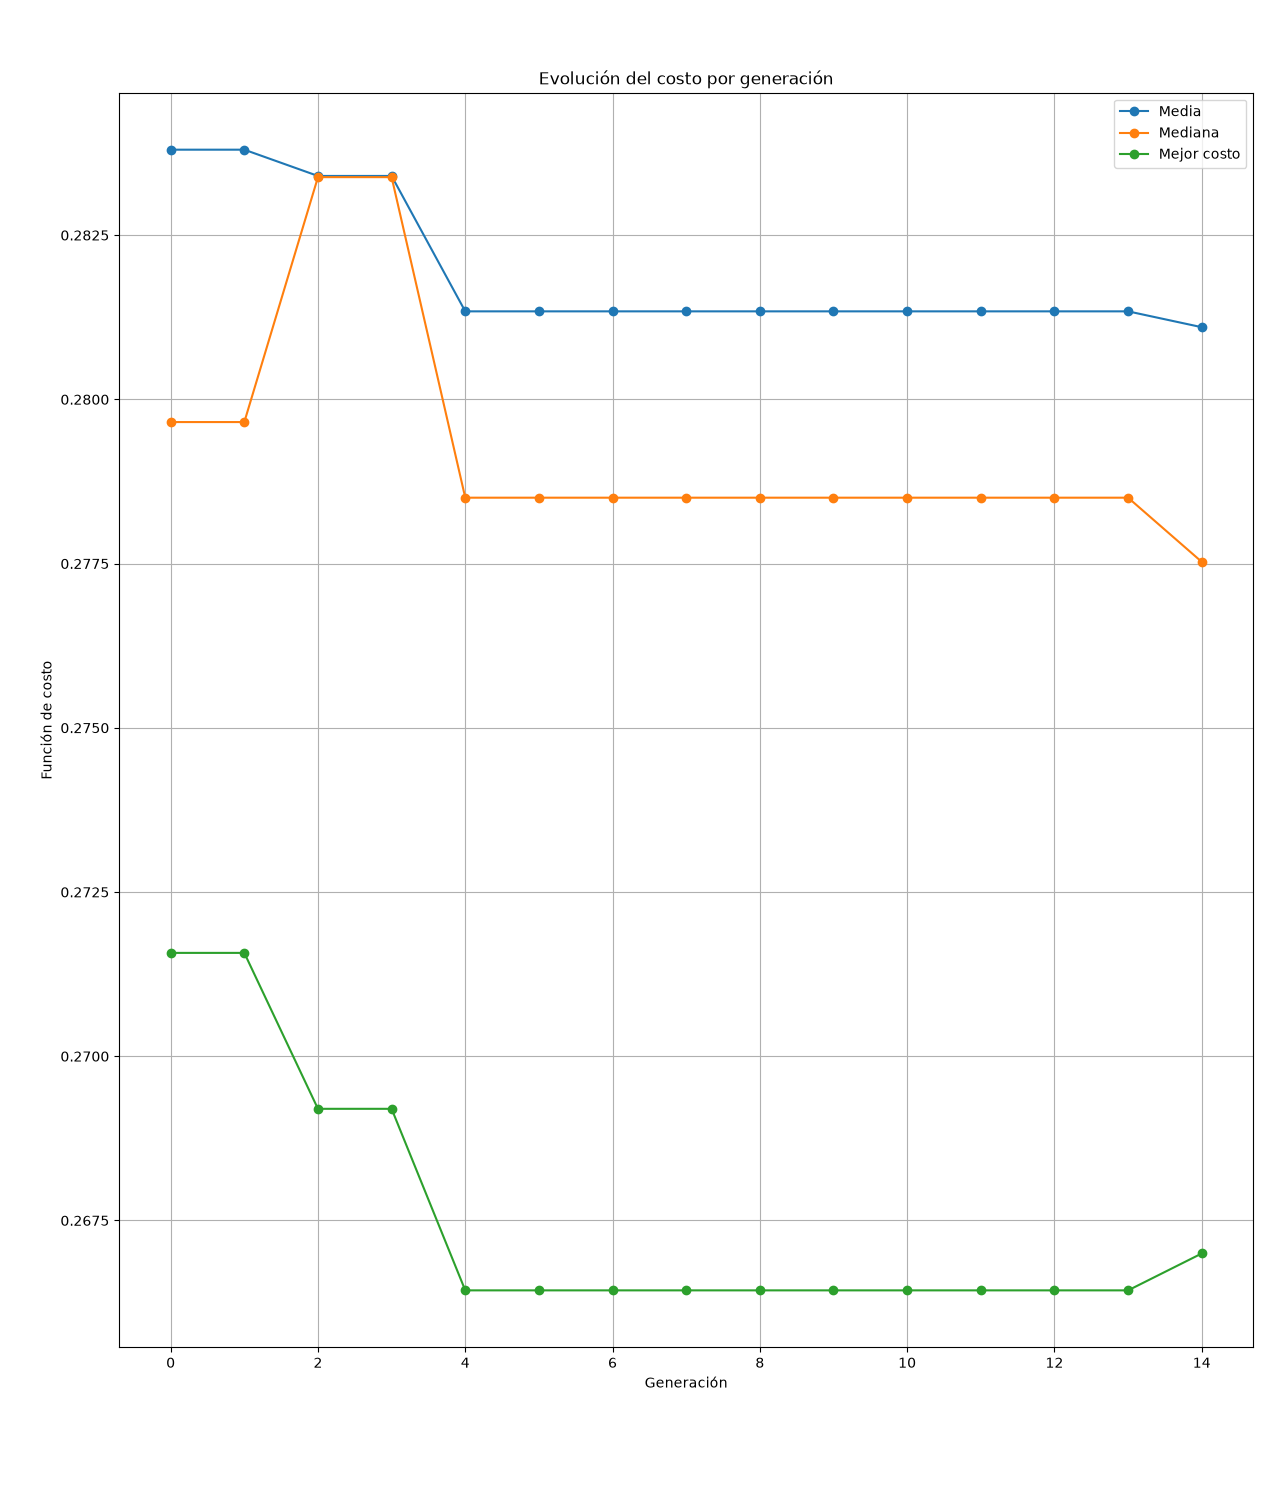
\includegraphics[
        width=0.80\textwidth,
        height=0.43\textheight,
        keepaspectratio
    ]{images/EvolucionMejorCosto.png}
    \caption{Media, mediana y mejor costo de la configuración campeona
    de cada generación. Estas curvas no representan las estadísticas
    de todas las corridas de la generación ni el mínimo global acumulado.}
    \label{fig:evolucion-campeon40}
\end{figure}
Esta distinción explica el incremento de la curva de mejor costo
del campeón en la última generación de la
Figura~\ref{fig:evolucion-campeon40}: pasó de $0.2664360763$ a
$0.2669975562$, mientras su media disminuyó. El sistema conservó
el mínimo global de $0.2638195256$ independientemente de ese cambio.
\begin{figure}[htbp]
    \centering
    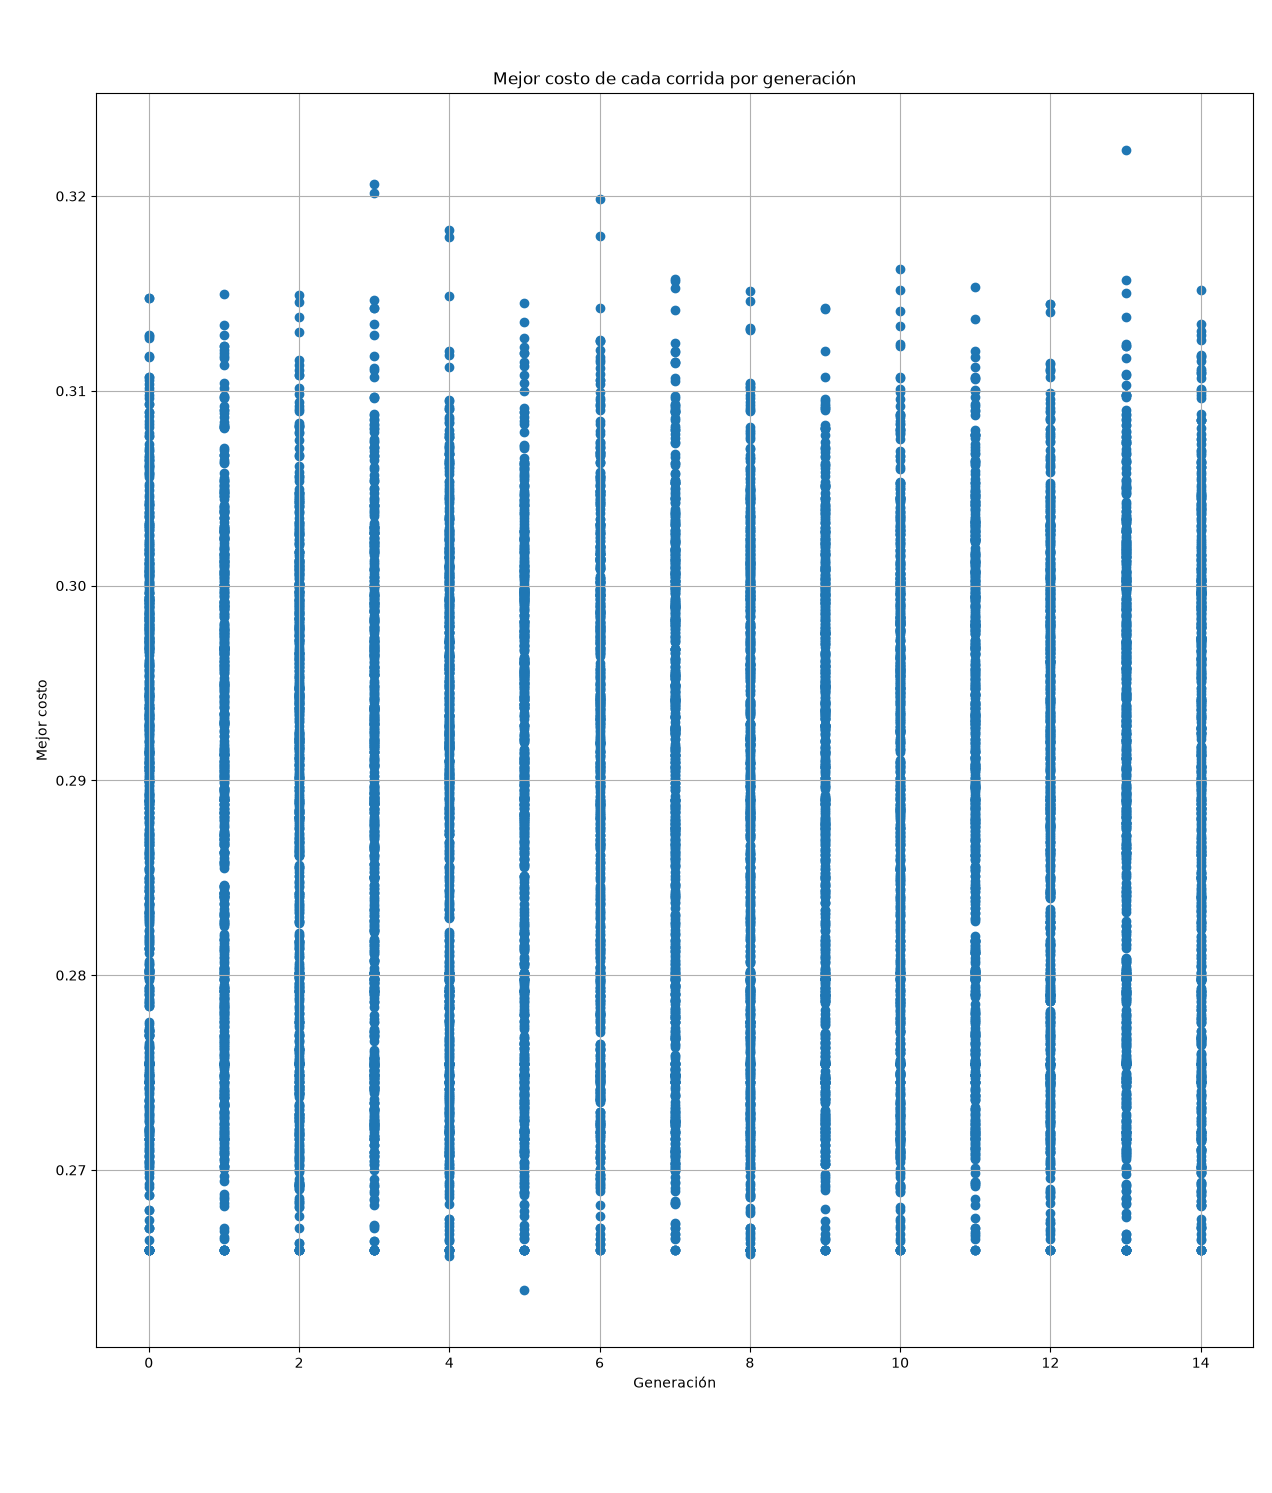
\includegraphics[
        width=0.80\textwidth,
        height=0.43\textheight,
        keepaspectratio
    ]{images/MejorCostoPorGeneracion.png}
    \caption{Mejor costo de cada corrida agrupado por generación.
    La dispersión persiste a lo largo de la experimentación.}
    \label{fig:dispersion-generaciones40}
\end{figure}

La Figura~\ref{fig:dispersion-generaciones40} muestra que la selección
adaptativa de parámetros no produjo una disminución uniforme de todos
los costos. La búsqueda siguió generando resultados diversos, incluso
después de identificar configuraciones competitivas.

\subsubsection{Relación entre parámetros, calidad y tiempo}

Las gráficas de dispersión permiten examinar asociaciones entre los
parámetros y el mejor costo. Sin embargo, varios parámetros y semillas
cambian simultáneamente, por lo que estas gráficas no permiten atribuir
causalmente una mejora a un parámetro aislado.
\begin{figure}[htbp]
    \centering
    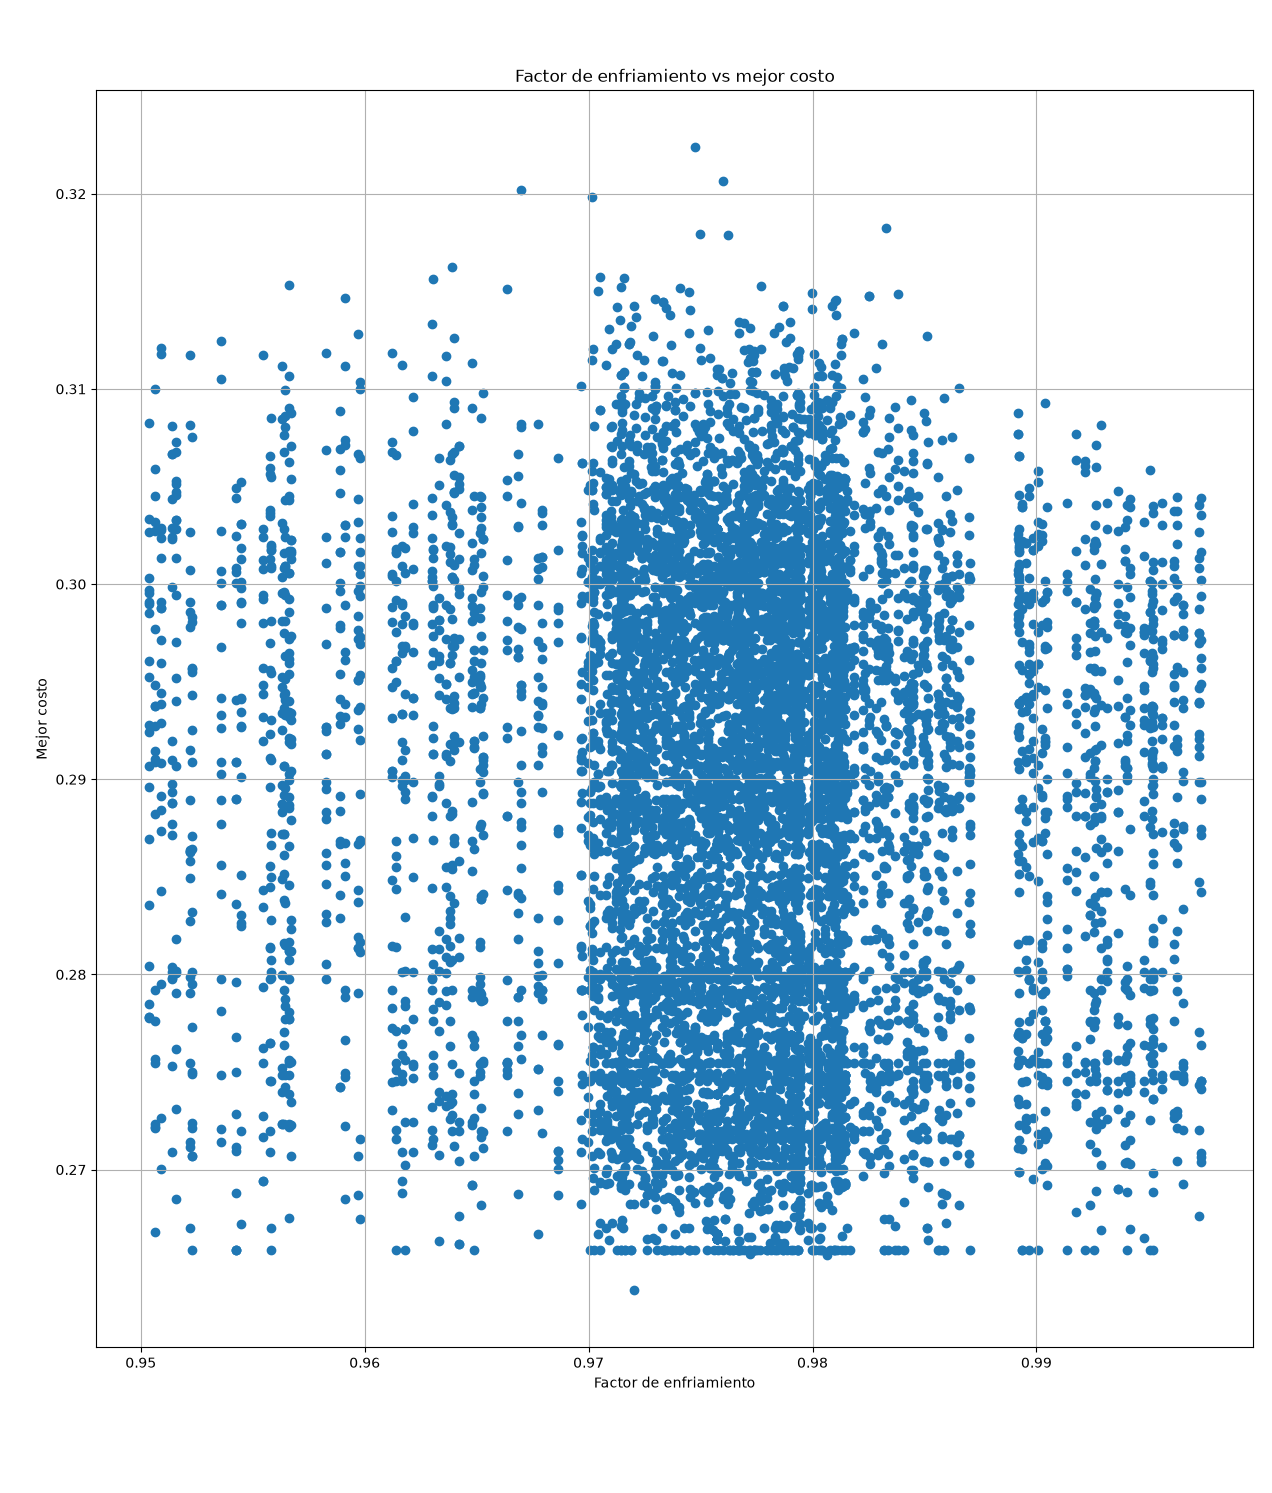
\includegraphics[width=0.48\textwidth]
        {images/FactorEnfriamenteMejorCosto.png}
    \hfill
    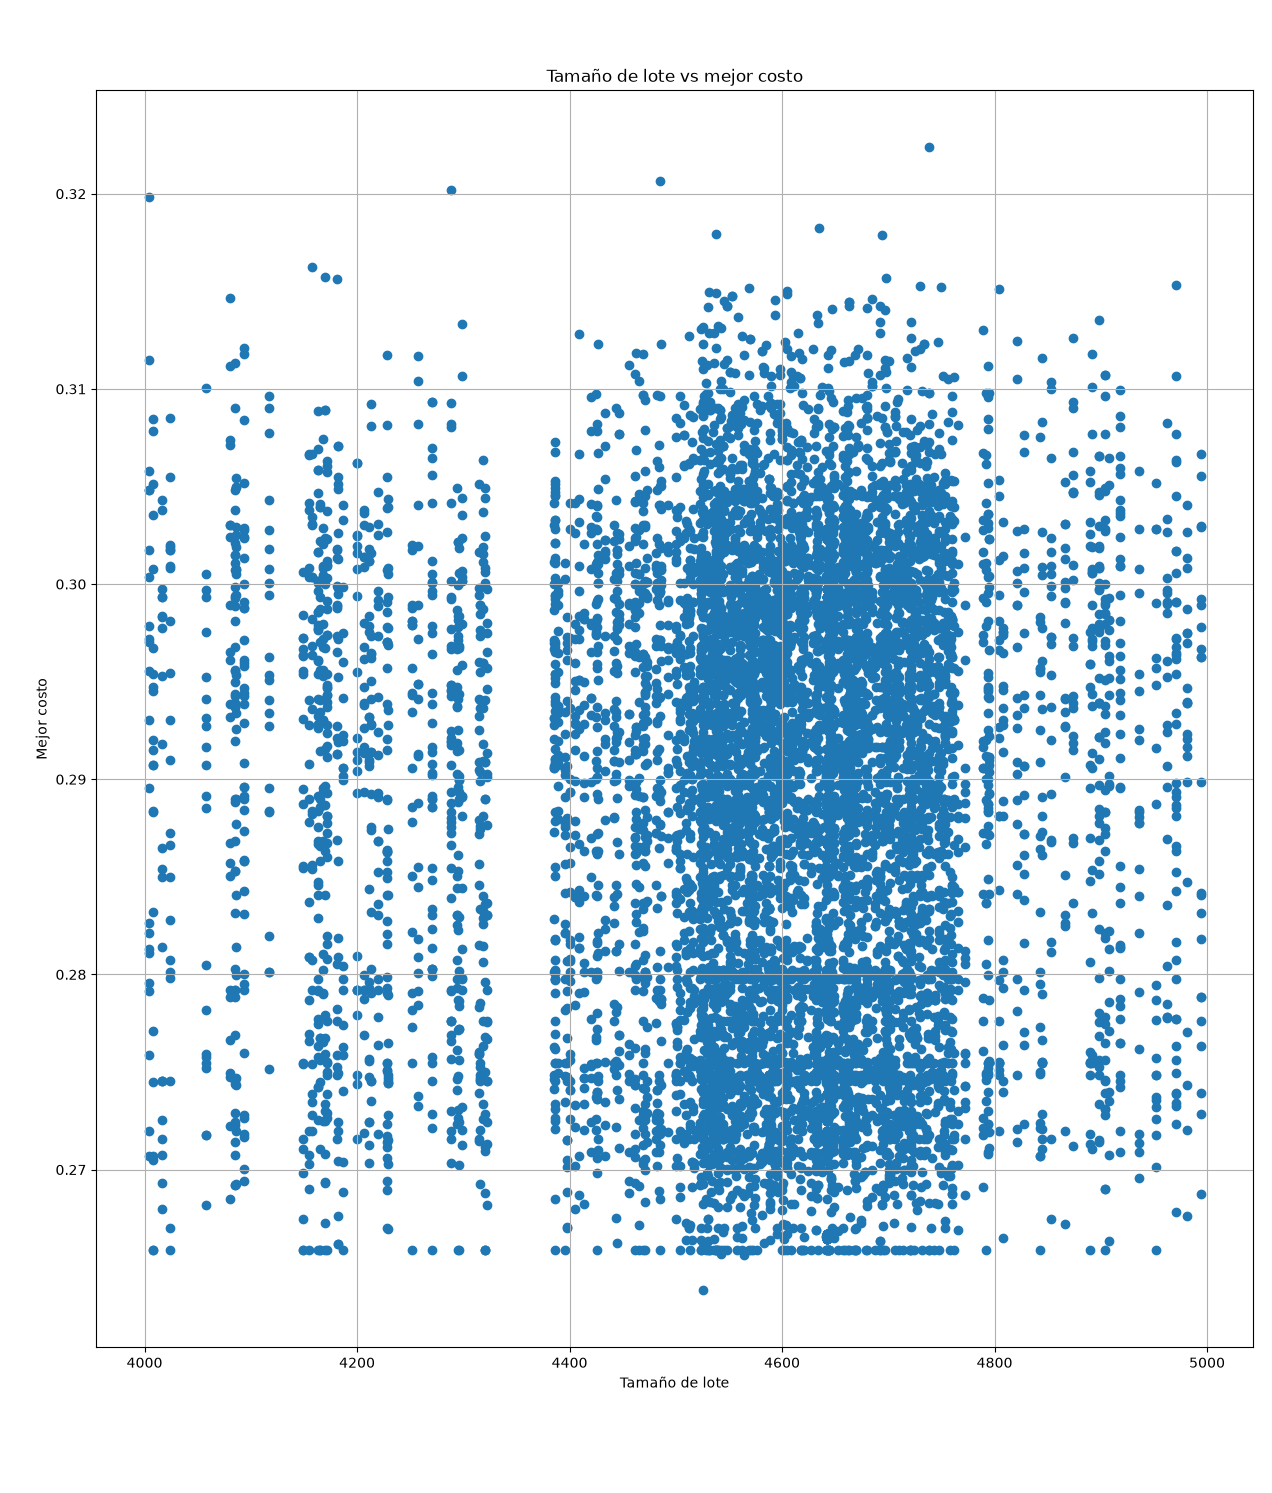
\includegraphics[width=0.48\textwidth]
        {images/LoteMejorCosto.png}
    \caption{Relación del mejor costo con el factor de enfriamiento
    y con el tamaño del lote.}
    \label{fig:enfriamiento-lote40}
\end{figure}
\\\\
En la Figura~\ref{fig:enfriamiento-lote40} se observan costos distintos
para valores semejantes del factor de enfriamiento y del tamaño de
lote. El mínimo global se obtuvo con $\alpha\approx0.9720$ y
$L=4526$, pero ello no demuestra que dichos valores sean óptimos
para todas las semillas.
\\
La concentración de puntos en ciertas regiones refleja también el
mecanismo de generación de candidatos alrededor del campeón.
En consecuencia, una mayor densidad de observaciones no debe
interpretarse por sí sola como evidencia de mayor calidad.
\begin{figure}[htbp]
    \centering
    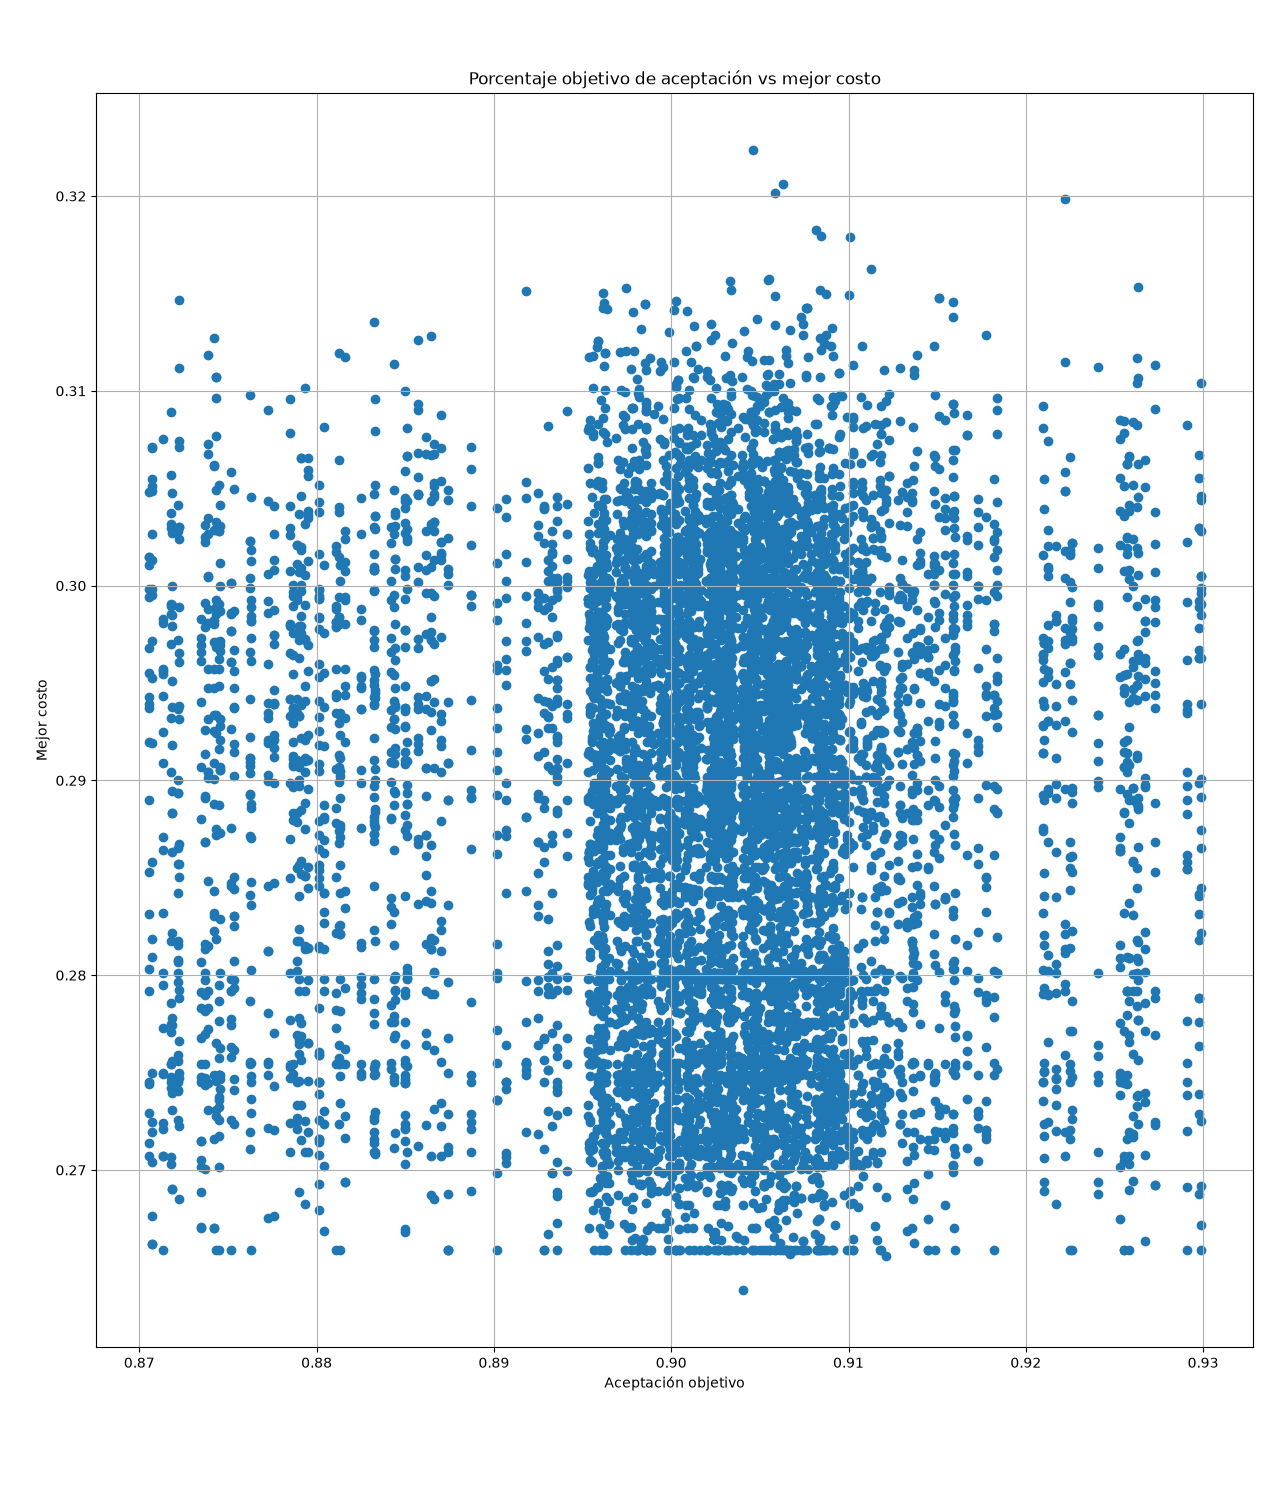
\includegraphics[width=0.48\textwidth]
        {images/ProcentajeAceptacionMejorCosoto.png}
    \hfill
    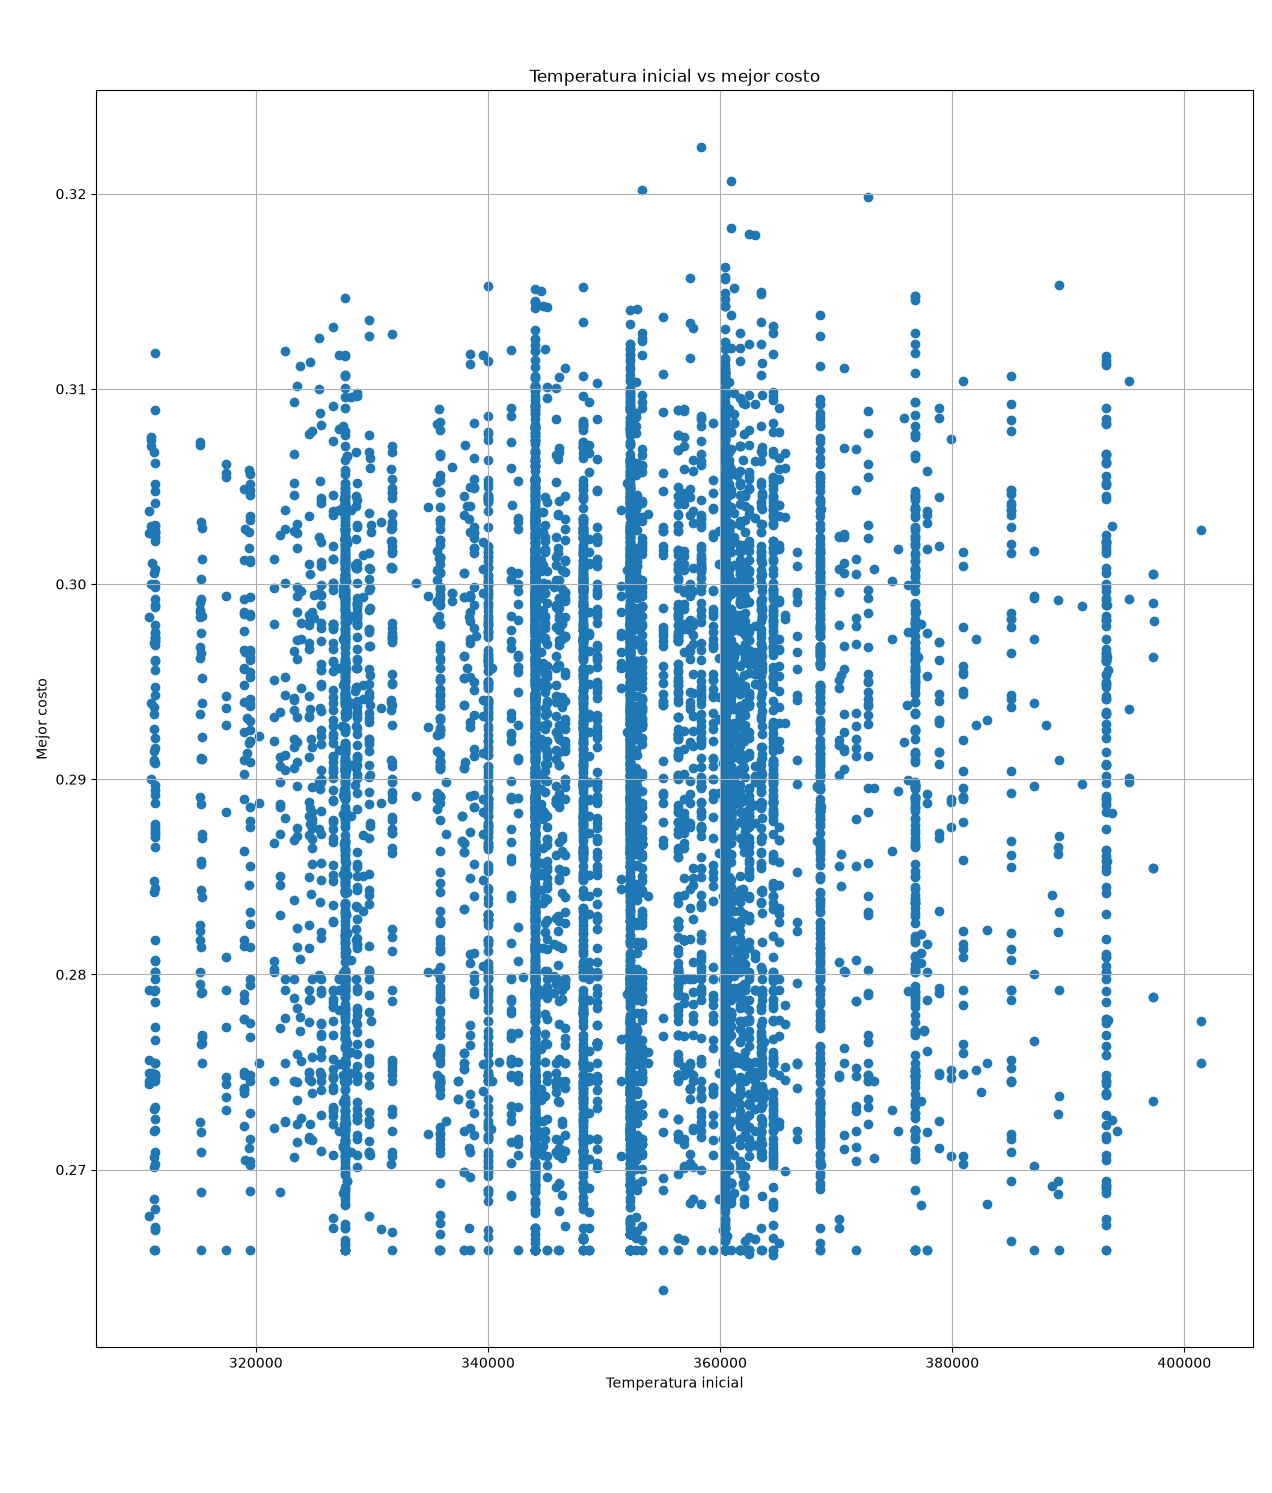
\includegraphics[width=0.48\textwidth]
        {images/TmpertauraInicialMejorCosto.png}
    \caption{Aceptación objetivo y temperatura inicial frente al mejor
    costo. La temperatura depende de la calibración y de su semilla.}
    \label{fig:temperatura-aceptacion40}
\end{figure}
\\\\
La Figura~\ref{fig:temperatura-aceptacion40} tampoco muestra una
relación monótona simple: temperaturas iniciales o proporciones
objetivo mayores no garantizan menores costos.
\begin{figure}[htbp]
    \centering
    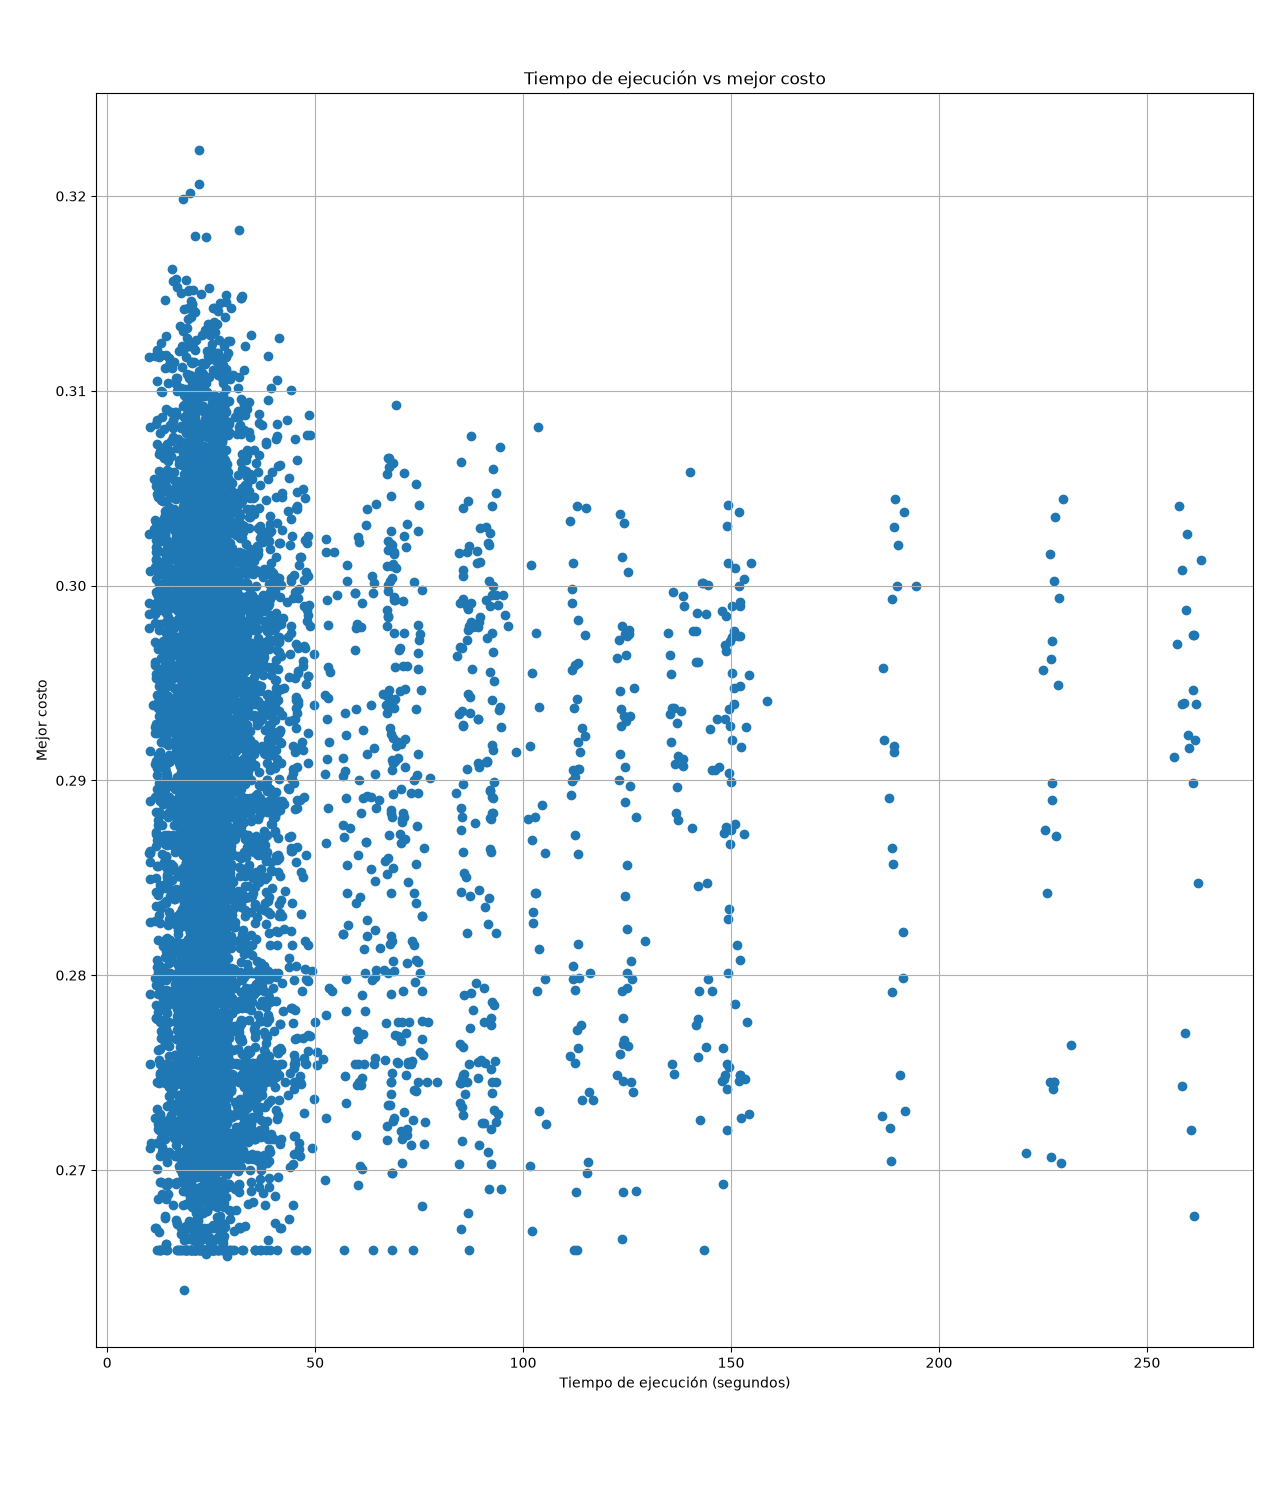
\includegraphics[
        width=0.80\textwidth,
        height=0.43\textheight,
        keepaspectratio
    ]{images/MejorCostoTiempo.png}
    \caption{Tiempo de optimización y mejor costo de cada corrida.}
    \label{fig:tiempo-costo40}
\end{figure}
En particular, la mejor corrida requirió aproximadamente
$18.57$ segundos, mientras que algunas ejecuciones superaron los
$250$ segundos sin alcanzar ese mínimo
(Figura~\ref{fig:tiempo-costo40}). En este experimento, dedicar más
tiempo a una corrida no aseguró una solución mejor.

\subsubsection{Trayectoria de las evaluaciones aceptadas}

El archivo de evaluaciones contiene $6160177$ valores, cantidad
que coincide con el número de vecinos aceptados de la corrida
ganadora. Su mínimo es
\[
    0.26381952559689636,
\]
y su último valor es
\[
    0.27099373796177584.
\]
Ambos coinciden con los costos registrados en el reporte experimental.
\\\\
El mínimo aparece por primera vez en la evaluación aceptada
\[
    j=6047891,
\]
aproximadamente al $98.18\%$ de la secuencia de aceptaciones.
Esta posición no equivale al mismo porcentaje del tiempo de ejecución,
pues entre dos aceptaciones puede existir un número variable de
intentos rechazados.
\begin{figure}[htbp]
    \centering
    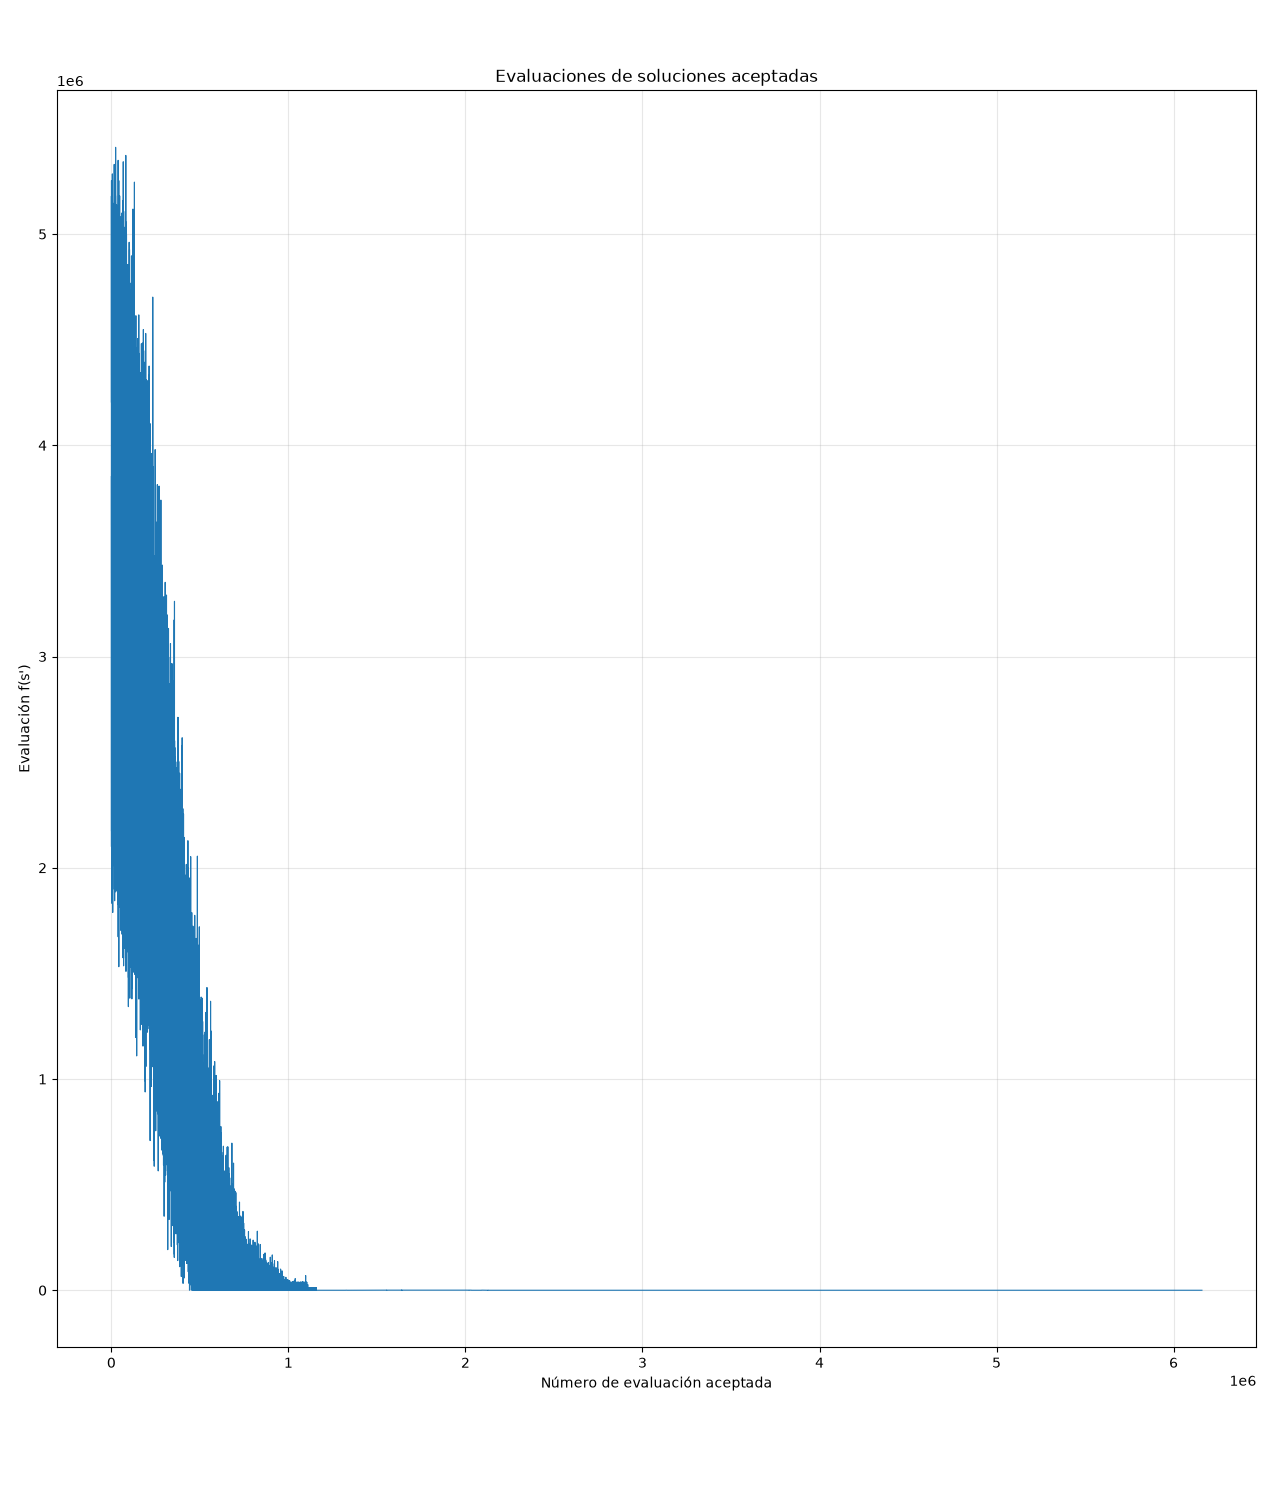
\includegraphics[
        width=0.80\textwidth,
        height=0.40\textheight,
        keepaspectratio
    ]{images/EvaluacionesGeneral.png}
    \caption{Evolución de los costos de las soluciones aceptadas.
    La escala global permite observar la reducción de los costos
    elevados, pero oculta las diferencias pequeñas de la etapa final.}
    \label{fig:evaluaciones40}
\end{figure}
\\\\
Los valores iniciales elevados son compatibles con la presencia de
penalizaciones por conexiones inexistentes. Posteriormente, la
trayectoria alcanza costos mucho menores. La apariencia cercana a
cero de la parte final de la Figura~\ref{fig:evaluaciones40} se debe
a la escala vertical y no significa que el costo se anule.
\\
La secuencia de costos aceptados puede aumentar o disminuir; solamente
el mínimo acumulado es no creciente. Por ello, una estabilización
visual de la trayectoria final no implica que su último valor sea
el mejor de toda la corrida.

\subsubsection{Representación geográfica de la mejor ruta}

La Figura~\ref{fig:mapa40} muestra la representación geográfica
de la ruta asociada al mínimo global. 
\\\\
El mapa permite inspeccionar
el orden de visita y la distribución espacial de las 40 ciudades.
\begin{figure}[htbp]
    \centering
    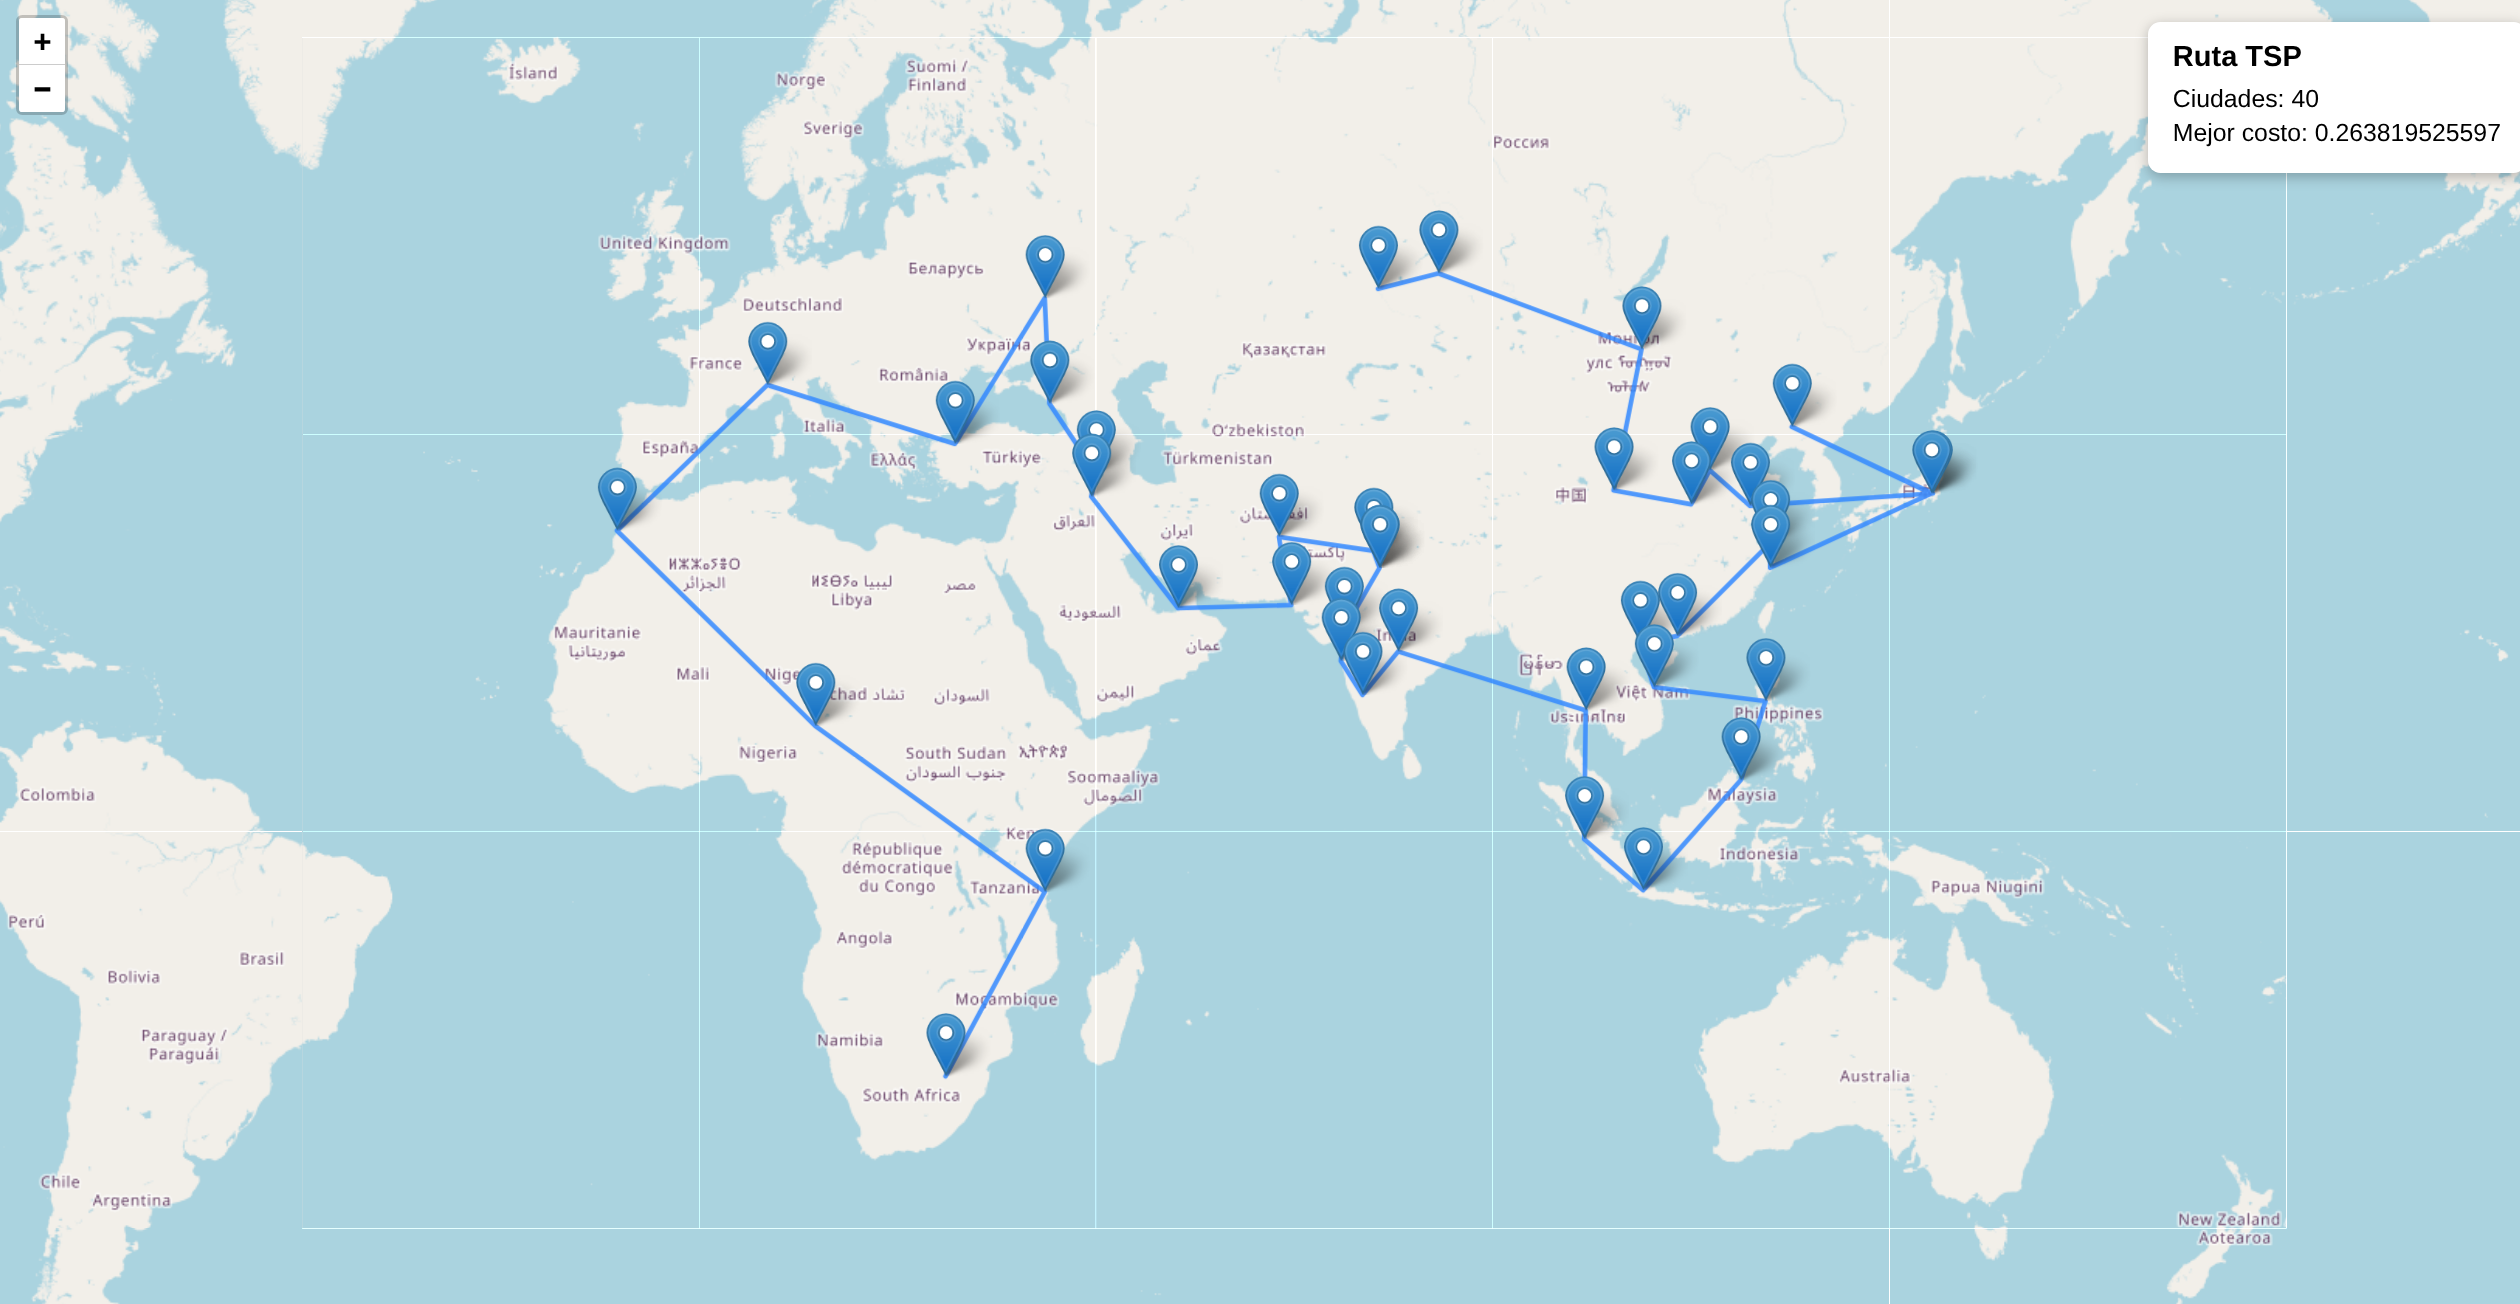
\includegraphics[width=\textwidth]{images/MapaRuta40.png}
    \caption{Representación geográfica de la mejor ruta encontrada
    para 40 ciudades, con costo normalizado $0.2638195256$.
    Mapa base: OpenStreetMap y sus colaboradores.}
    \label{fig:mapa40}
\end{figure}
\\\\
Las líneas representan conexiones entre ciudades consecutivas de la
permutación y no necesariamente trayectos por carretera. Conforme a
la función objetivo implementada, se consideran 39 conexiones y
no se exige regresar de la última ciudad a la primera.
\\
El mapa complementa el análisis numérico, pero no certifica la
optimalidad ni permite comprobar por sí solo que todas las
conexiones pertenezcan a la gráfica original.

\subsubsection{Alcance de los resultados}

El experimento permitió encontrar una solución de costo
$0.2638195256$ y documentar su reproducción mediante semillas y
parámetros explícitos. También mostró que seleccionar configuraciones
por media y buscar el menor costo individual son objetivos distintos.
\\
Las conclusiones se restringen a esta instancia de 40 ciudades y a
los intervalos explorados. 
\\
La repetición de semillas y campeones,
junto con la selección adaptativa de candidatos, impide tratar las
9900 corridas como observaciones independientes de una misma
distribución. Las medias y medianas presentadas describen los
registros obtenidos, sin constituir una garantía de desempeño para
otras instancias o semillas.
\\\\
Finalmente, al no disponer de una solución óptima certificada,
el resultado debe presentarse como el mejor encontrado durante
la experimentación, y no como el óptimo del problema.


\subsection{Instancia de 150 ciudades}
\label{subsec:resultados150}

El mejor costo obtenido por el sistema de Aceptación por Umbrales
para la instancia de 150 ciudades fue
\[    \boxed{f_{\min}=0.13945992054852843}.
\]
Este resultado apareció en la generación 1 del experimento original,
con semilla base 123 y semilla de ejecución 247. El valor corresponde a la función objetivo normalizada del proyecto.

\subsubsection{Resultados generales del experimento original}

La Tabla~\ref{tab:resultados150-general} resume las 1717 corridas
registradas antes de la interrupción.
\begin{table}[htbp]
    \centering
    \small
    \begin{tabular}{lr}
        \hline
        Medida & Valor \\
        \hline
        Corridas registradas & 1717 \\
        Generaciones completas & 5 \\
        Corridas de la generación parcial & 217 \\
        Mejor costo & $0.1394599205$ \\
        Mediana de los mejores costos & $0.1605503867$ \\
        Media de los mejores costos & $914.0177446037$ \\
        Mayor mejor costo registrado & $41081.6643501569$ \\
        Corridas con mejor costo menor que $1$ & 1666 \\
        Corridas con mejor costo mayor o igual que $1$ & 51 \\
        Corridas con mejor costo menor que $0.14$ & 1 \\
        \hline
    \end{tabular}
    \caption{Estadísticas descriptivas del experimento original
    de 150 ciudades. Cada observación es el mejor costo de una corrida.}
    \label{tab:resultados150-general}
\end{table}
\\\\
La media quedó fuertemente influida por los costos extremos.
Por ello, su valor no describe adecuadamente la región en la que se
concentró la mayoría de las corridas. La mediana, cercana a $0.1606$,
complementa esta información.
\\\\
Al considerar únicamente las 1666 corridas cuyo mejor costo fue
menor que $1$, la media fue $0.1605081366$. Este valor es una
estadística condicionada a dicho filtro y no sustituye a la media
del conjunto completo. Tampoco se utiliza el umbral $1$, por sí solo,
como comprobación de la factibilidad de cada ruta.
\\
Solo una de las 1717 corridas obtuvo un costo menor que $0.14$.
El resultado excepcional debe distinguirse, por tanto, del
comportamiento habitual de las configuraciones evaluadas.
\\
La suma de los tiempos registrados por el algoritmo fue de
$513678.83$ segundos, aproximadamente 142 horas y 41 minutos.
Esta cifra excluye la calibración de temperaturas y otros costos
del proceso, y no debe confundirse con su duración total.

\subsubsection{Evolución de la mejor solución global}

El reporte de mejores soluciones registra seis actualizaciones
del récord, mostradas en la Tabla~\ref{tab:resultados150-records}.
\begin{table}[htbp]
    \centering
    \small
    \begin{tabular}{ccr}
        \hline
        Generación & Semilla base & Nuevo mejor costo global \\
        \hline
        0 & 123 & $0.1444527028$ \\
        0 & 789 & $0.1439389451$ \\
        0 & 456 & $0.1429565150$ \\
        0 & 658 & $0.1426423516$ \\
        0 & 123 & $0.1404900529$ \\
        1 & 123 & $\mathbf{0.1394599205}$ \\
        \hline
    \end{tabular}
    \caption{Actualizaciones de la mejor solución global
    en el experimento original.}
    \label{tab:resultados150-records}
\end{table}
\\
Después de encontrar el récord en la generación 1, ninguna de las
corridas restantes registradas lo superó. Esto evidencia una
ausencia de mejoras dentro del presupuesto ejecutado, pero no
constituye una demostración de optimalidad.

\subsubsection{Campeón por media y mejor corrida individual}

La configuración campeona fue la misma en las cinco generaciones
completas. Su media fue $0.1528260732$, su mediana $0.1522480126$
y su mejor corrida $0.1437814907$.
\\\\
La Figura~\ref{fig:150-evolucion-campeon} representa estas estadísticas
del campeón. Sus líneas constantes no significan que todas las
corridas fueran iguales ni que el récord global no cambiara.
Indican que ninguna configuración desplazó al campeón bajo el
criterio de selección por media.
\begin{figure}[htbp]
    \centering
    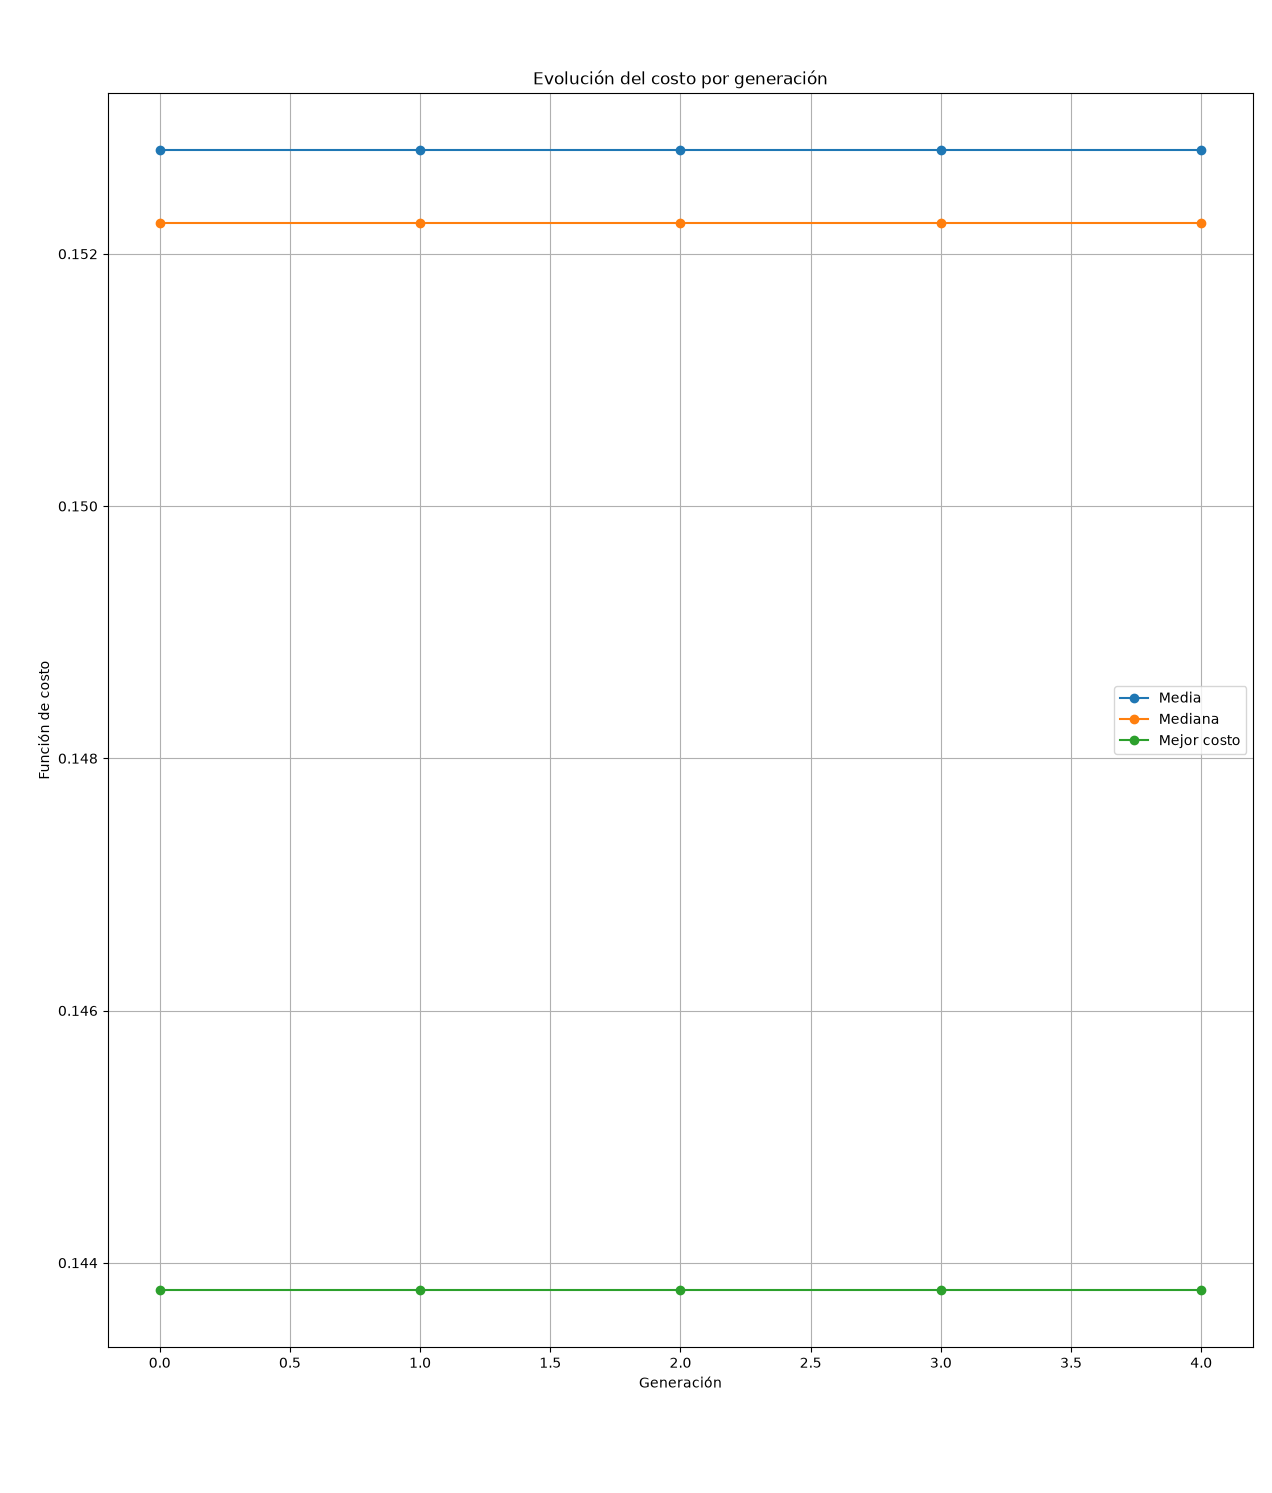
\includegraphics[width=0.76\textwidth]
        {images/EvolucionCostoGen150.png}
    \caption{Media, mediana y mejor costo de la configuración
    campeona en las generaciones completas. La figura no representa
    el mínimo global acumulado.}
    \label{fig:150-evolucion-campeon}
\end{figure}
\\
La configuración que produjo $0.1394599205$ tuvo una media de
$3376.1234793$ al evaluarse con las diez semillas de la generación 1.
Por ello, no fue seleccionada como campeona, aunque produjo la
mejor solución individual de todo el experimento.
\\
Este contraste muestra la diferencia entre los dos objetivos:
seleccionar parámetros con buen desempeño promedio y encontrar
el menor costo individual posible. El registro independiente
de la mejor solución global permitió conservar el récord a pesar
de que su configuración no resultó campeona.

\subsubsection{Configuración de la mejor corrida}

La Tabla~\ref{tab:resultados150-parametros} presenta los parámetros
necesarios para reproducir la mejor corrida.
\begin{table}[htbp]
    \centering
    \small
    \begin{tabular}{lr}
        \hline
        Parámetro & Valor \\
        \hline
        Semilla base & 123 \\
        Semilla para calcular $T_0$ & 246 \\
        Semilla de ejecución & 247 \\
        Temperatura inicial $T_0$ & $117760.0$ \\
        Factor de enfriamiento $\alpha$
            & $0.991148269450355$ \\
        Temperatura final $\varepsilon$
            & $1.487970391695277\times10^{-6}$ \\
        Tamaño del lote $L$ & 5493 \\
        Factor máximo de intentos $F$ & 76 \\
        Máximo de intentos por lote & 417468 \\
        Aceptación objetivo & $0.8862108379610587$ \\
        Tolerancia de aceptación & $0.0025$ \\
        Muestras para calcular $T_0$ & 5000 \\
        Máximo de iteraciones de calibración & 200 \\
        \hline
    \end{tabular}
    \caption{Configuración que produjo el mejor costo de
    Aceptación por Umbrales para 150 ciudades.}
    \label{tab:resultados150-parametros}
\end{table}
\\
La temperatura inicial elevada debe interpretarse en el contexto de
la función objetivo aumentada. La solución inicial tuvo un costo de
$6092371.48209038$, muy superior al costo de la mejor ruta encontrada.
La presencia de pesos penalizados permite que la función objetivo
alcance magnitudes elevadas aun después de la normalización.
\\
Los resultados operativos de la corrida fueron:
\[
\begin{aligned}
    N_{\mathrm{generados}} &= 814000800,\\
    N_{\mathrm{aceptados}} &= 24621160,\\
    N_{\mathrm{temperaturas}} &= 2816.
\end{aligned}
\]
La proporción global de vecinos aceptados fue aproximadamente
\[
    \frac{24621160}{814000800}\times100
    \approx 3.02\%.
\]
Esta proporción no debe confundirse con la aceptación objetivo de
$88.62\%$, utilizada únicamente para calibrar la temperatura inicial.
\\
En el experimento original se registraron $332.43$ segundos para
esta corrida. Una reproducción en modo normal reportó
$147.85$ segundos y obtuvo los mismos costos y contadores.
La diferencia temporal no debe atribuirse únicamente al modo de
ejecución, pues las mediciones corresponden a condiciones de
ejecución distintas.

\subsubsection{Distribución de resultados y parámetros}

La Figura~\ref{fig:150-costos-generacion} muestra los mejores costos
individuales por generación. Los valores extremos amplían
considerablemente la escala vertical y comprimen visualmente las
diferencias entre las soluciones de costo cercano a $0.14$--$0.17$.
\begin{figure}[htbp]
    \centering
    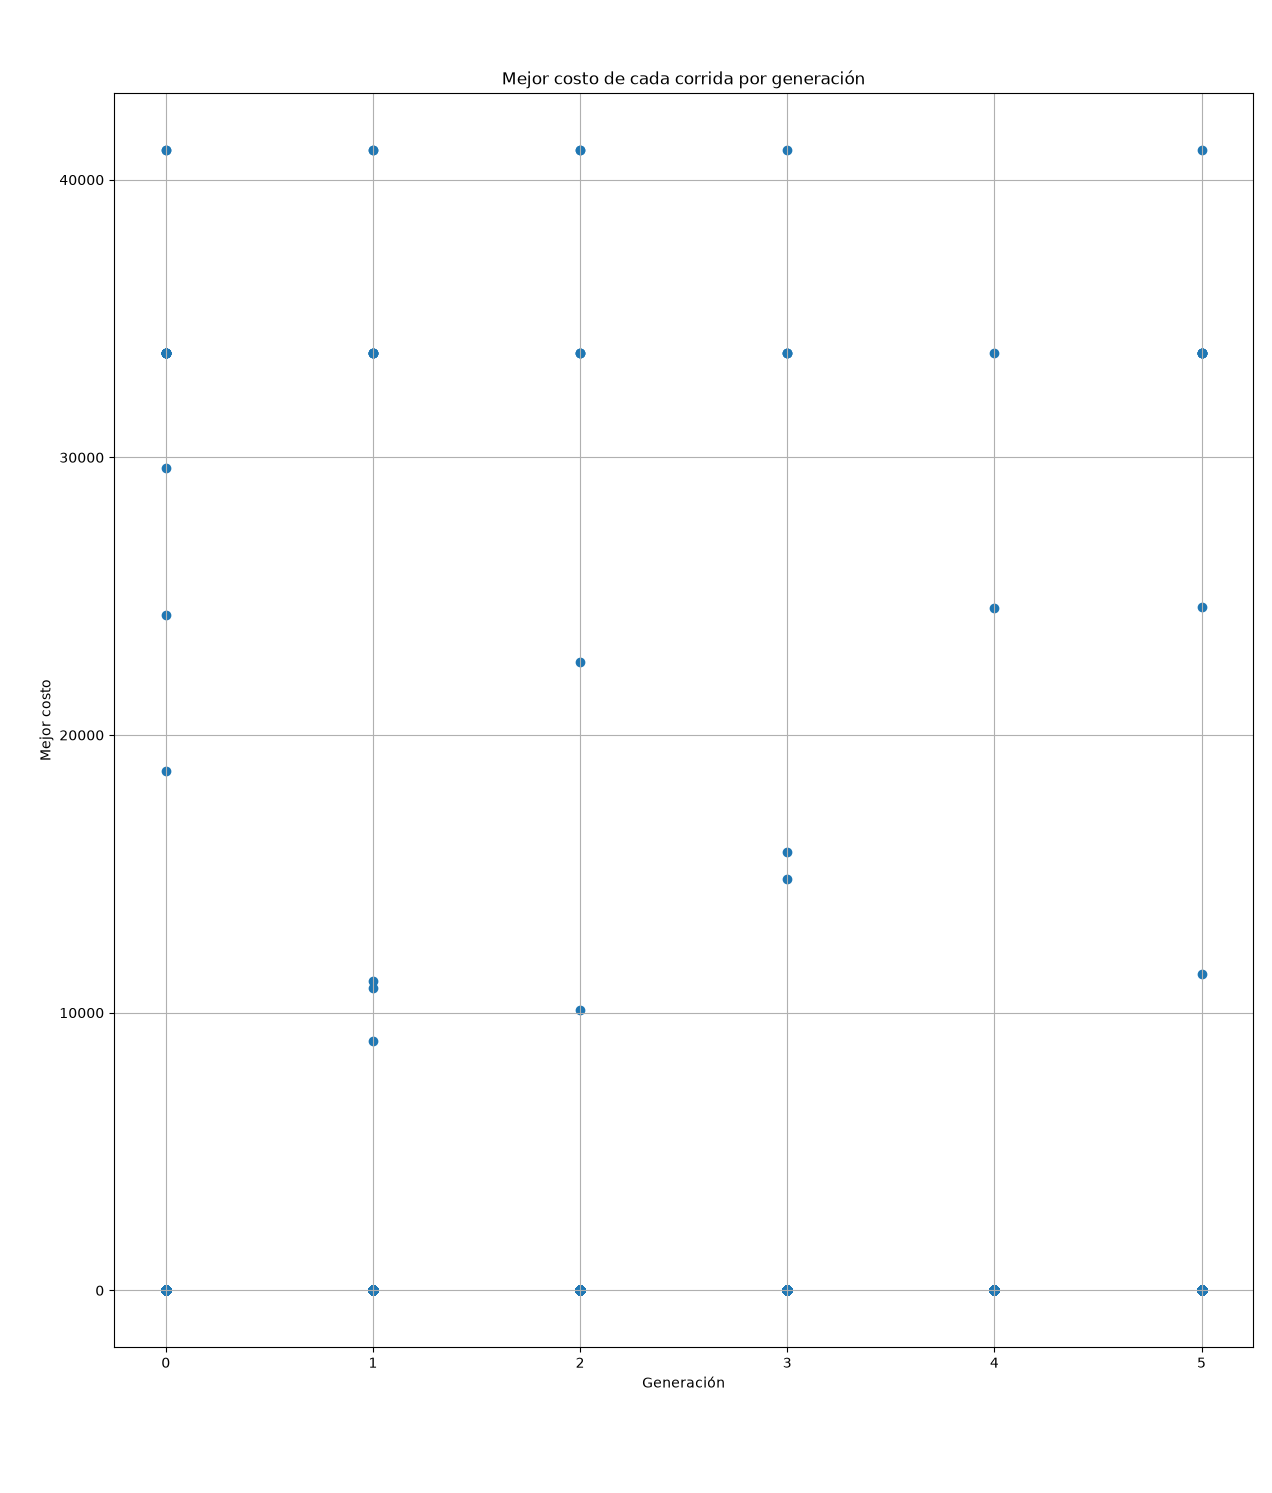
\includegraphics[width=0.76\textwidth]
        {images/MejorCostoPorGeneracion150}
    \caption{Mejor costo de cada corrida del experimento original.
    La generación 5 contiene únicamente 217 corridas, mientras que
    cada generación anterior contiene 300.}
    \label{fig:150-costos-generacion}
\end{figure}
\\
Las Figuras~\ref{fig:150-factor-lote} y
\ref{fig:150-aceptacion-temperatura} relacionan los resultados con
el enfriamiento, el tamaño de lote, la aceptación objetivo y la
temperatura inicial.
\begin{figure}[htbp]
    \centering
    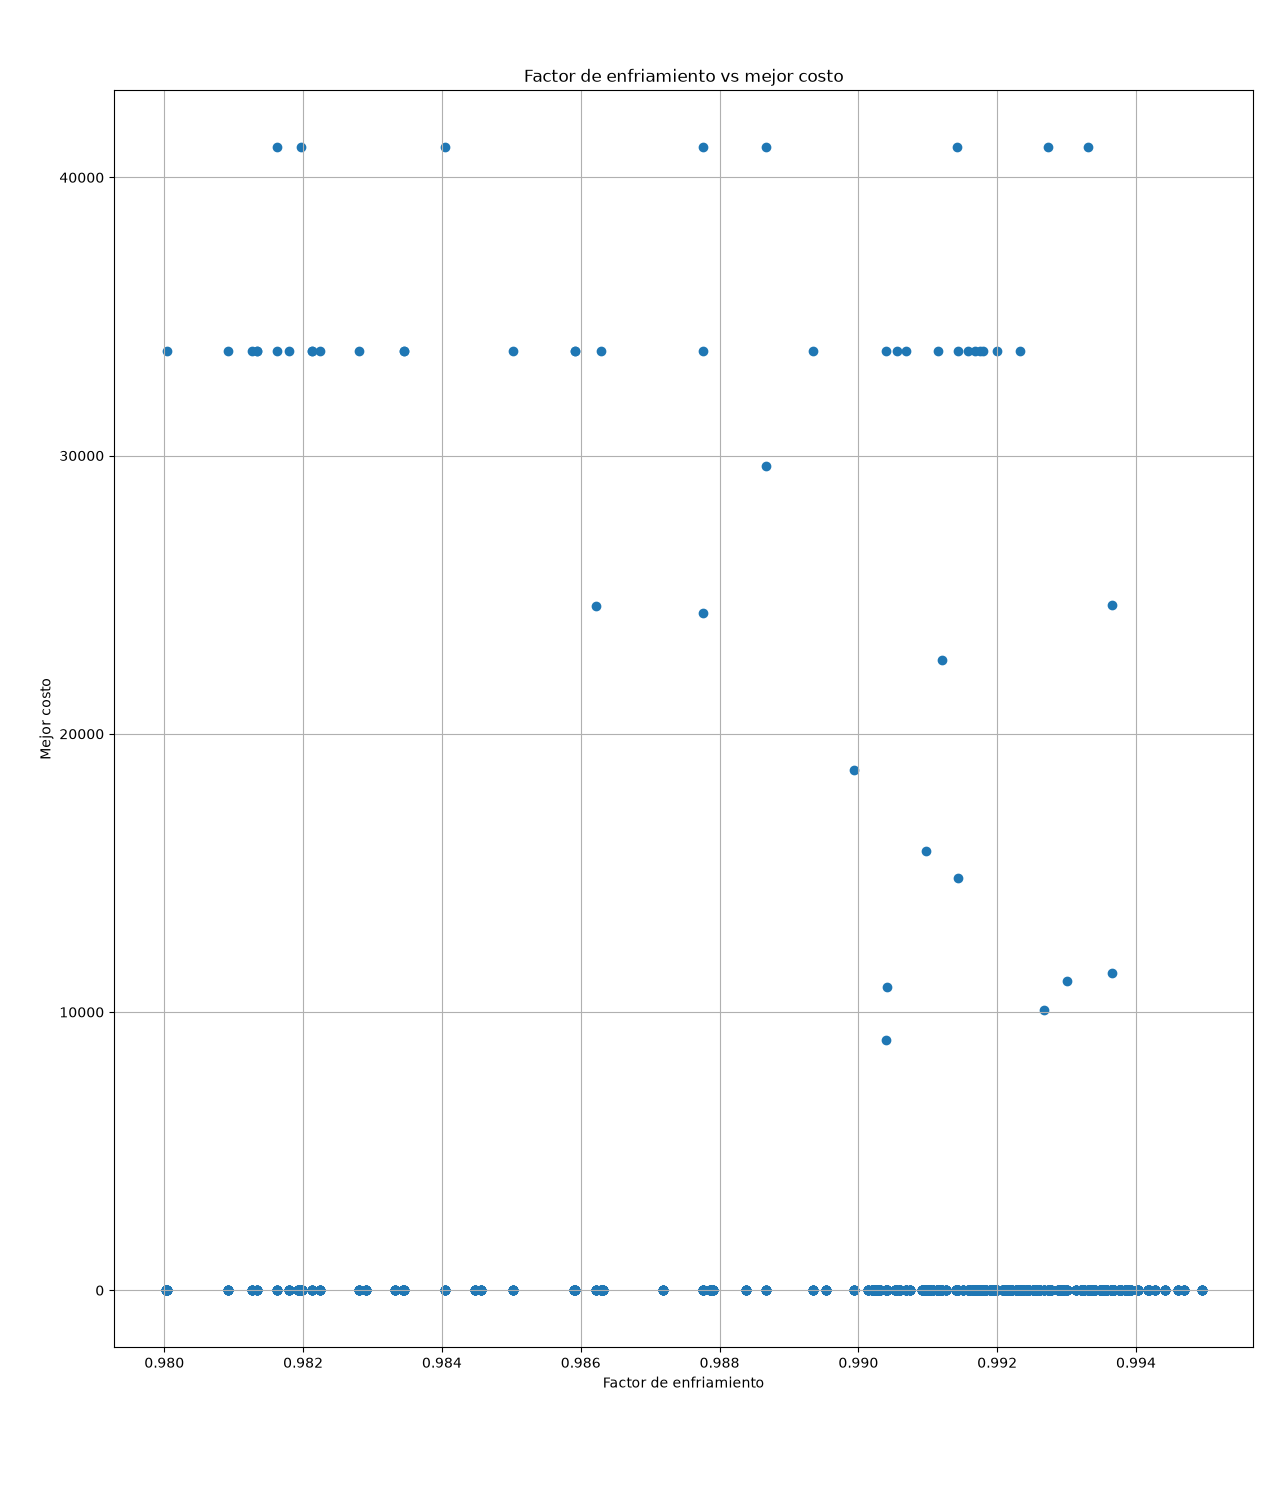
\includegraphics[width=0.48\textwidth]
        {images/FactorEnfrimientoMejorCosto150.png}
    \hfill
    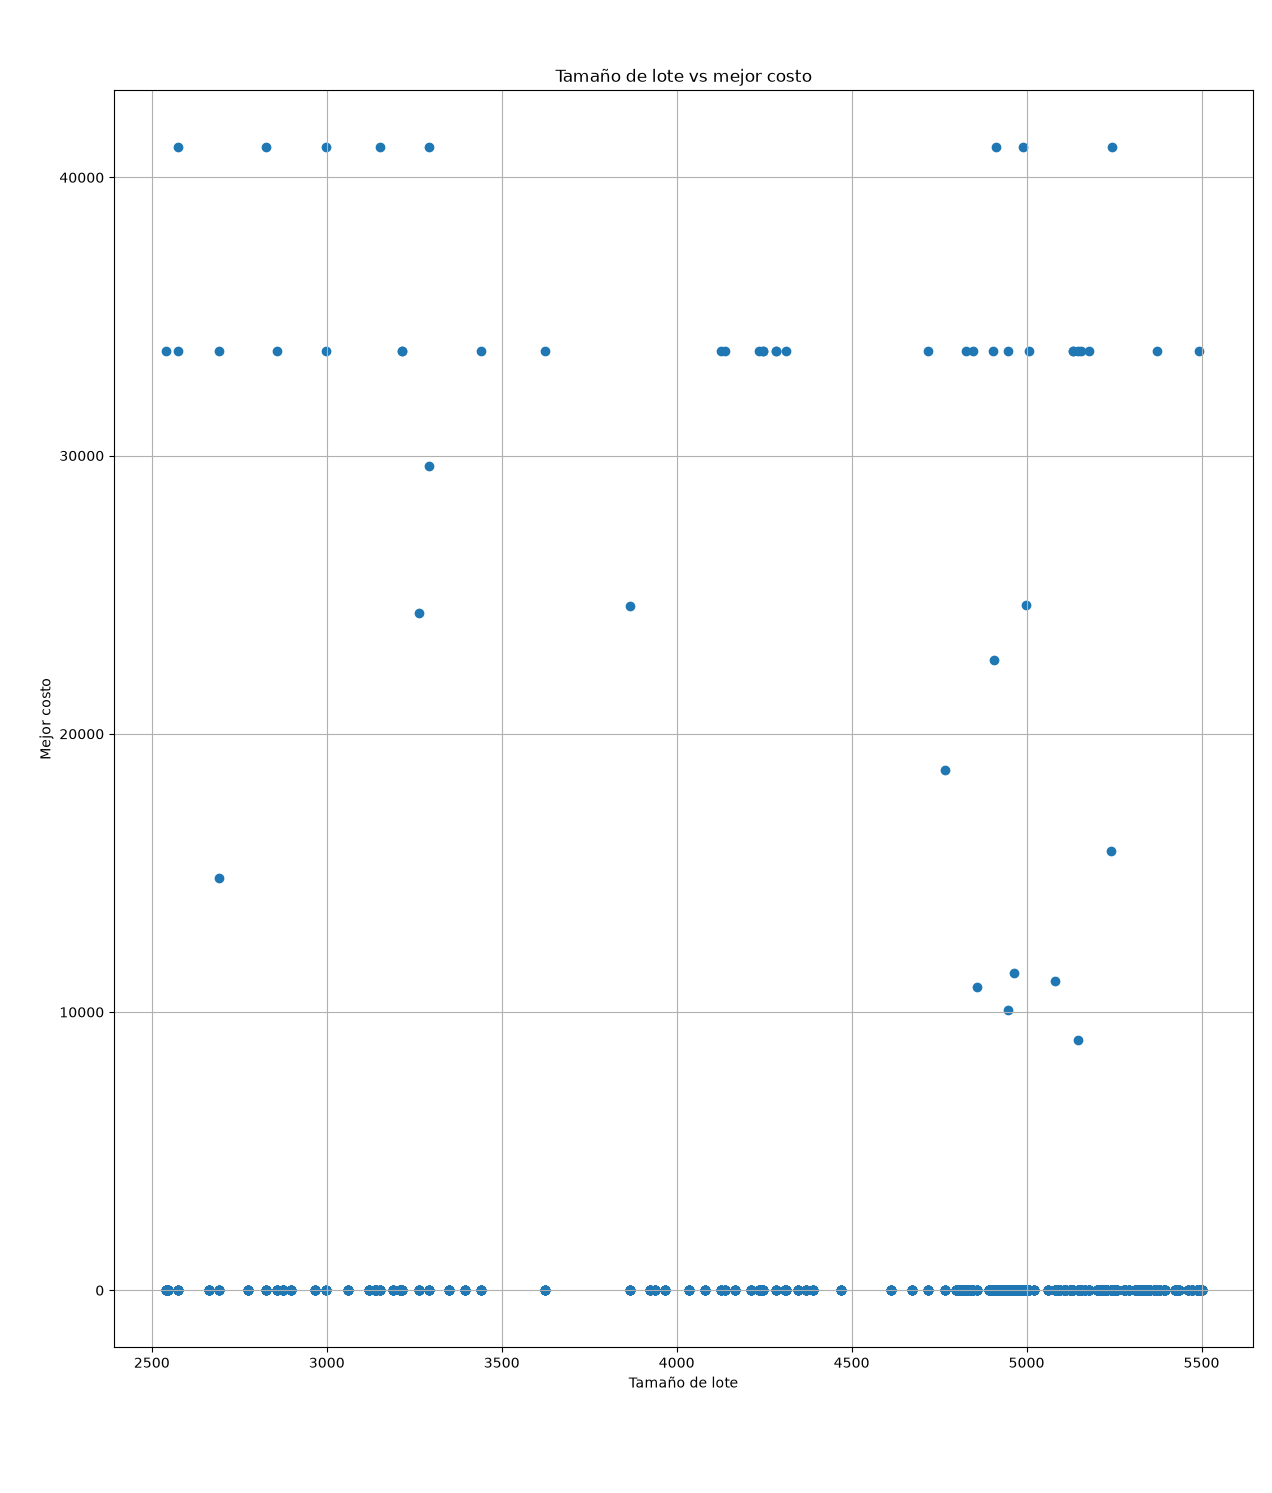
\includegraphics[width=0.48\textwidth]
        {images/MejroCostoLote150.png}
    \caption{Relación del mejor costo con el factor de enfriamiento
    y el tamaño del lote. Se muestran también los costos extremos.}
    \label{fig:150-factor-lote}
\end{figure}
\begin{figure}[htbp]
    \centering
    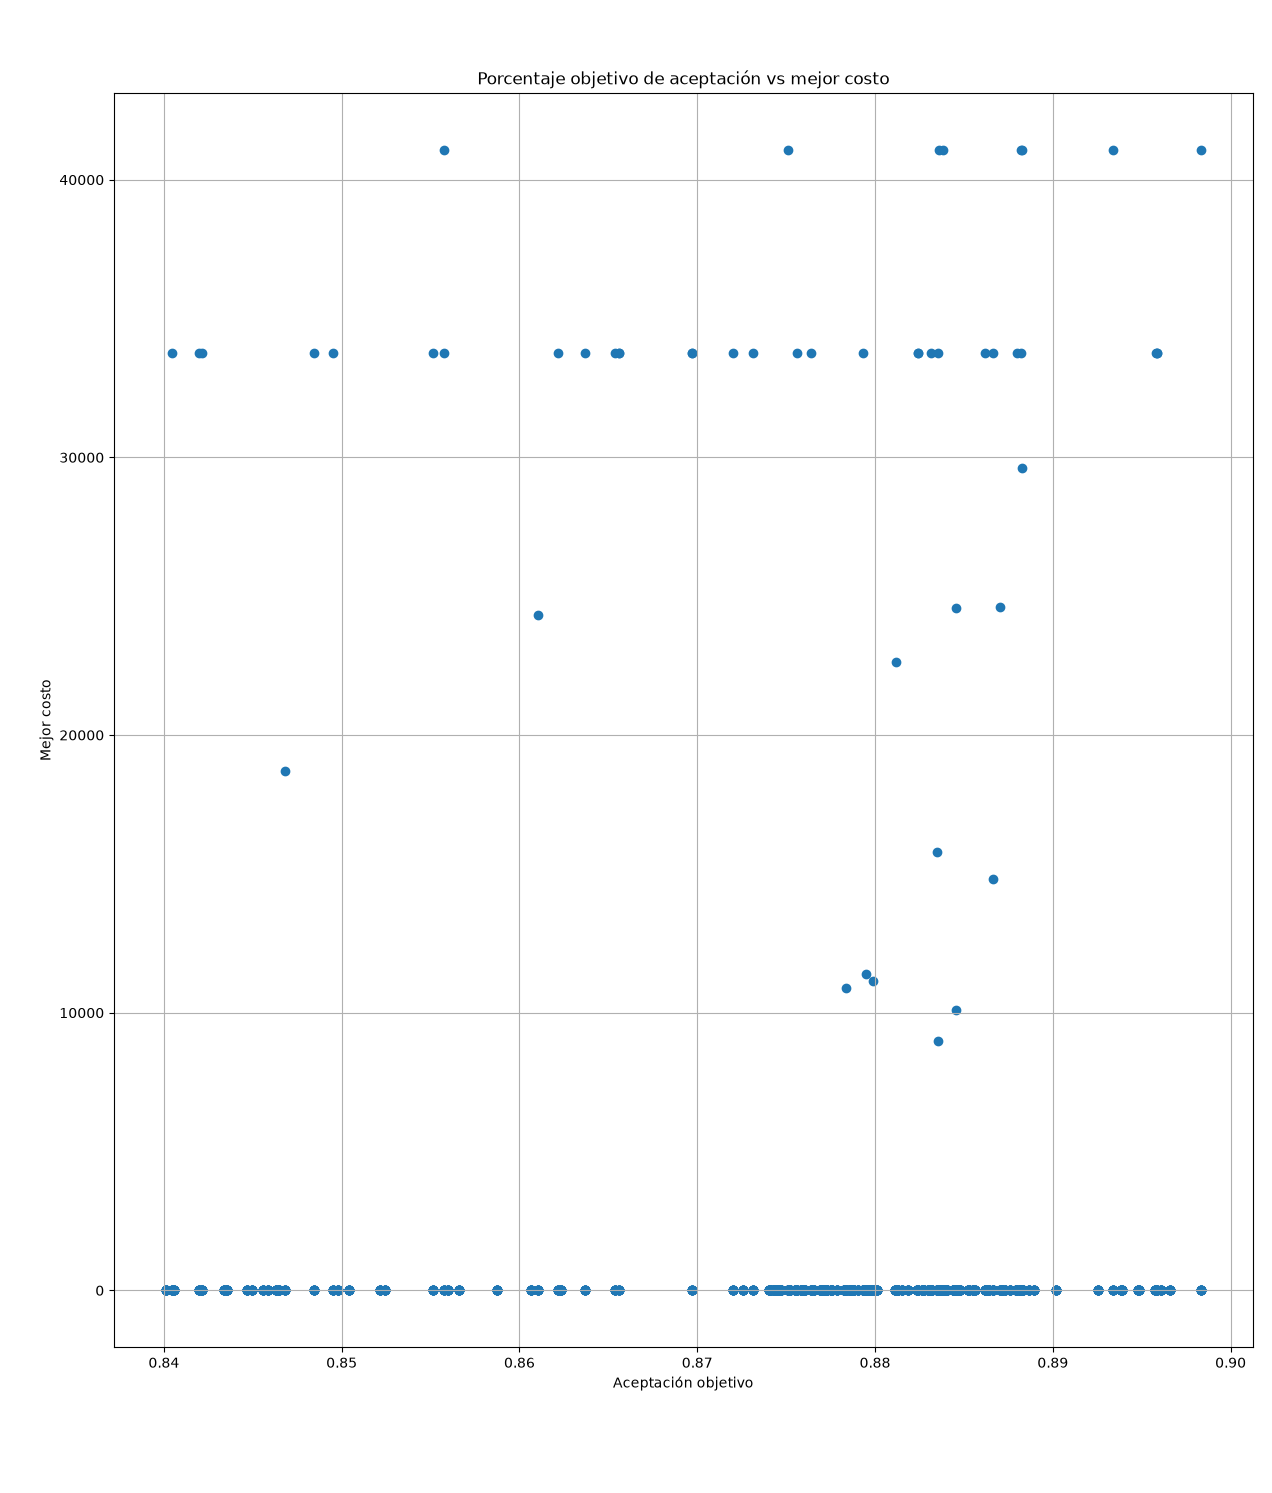
\includegraphics[width=0.48\textwidth]
        {images/ProcentajeAceptacionMejorCosto150.png}
    \hfill
    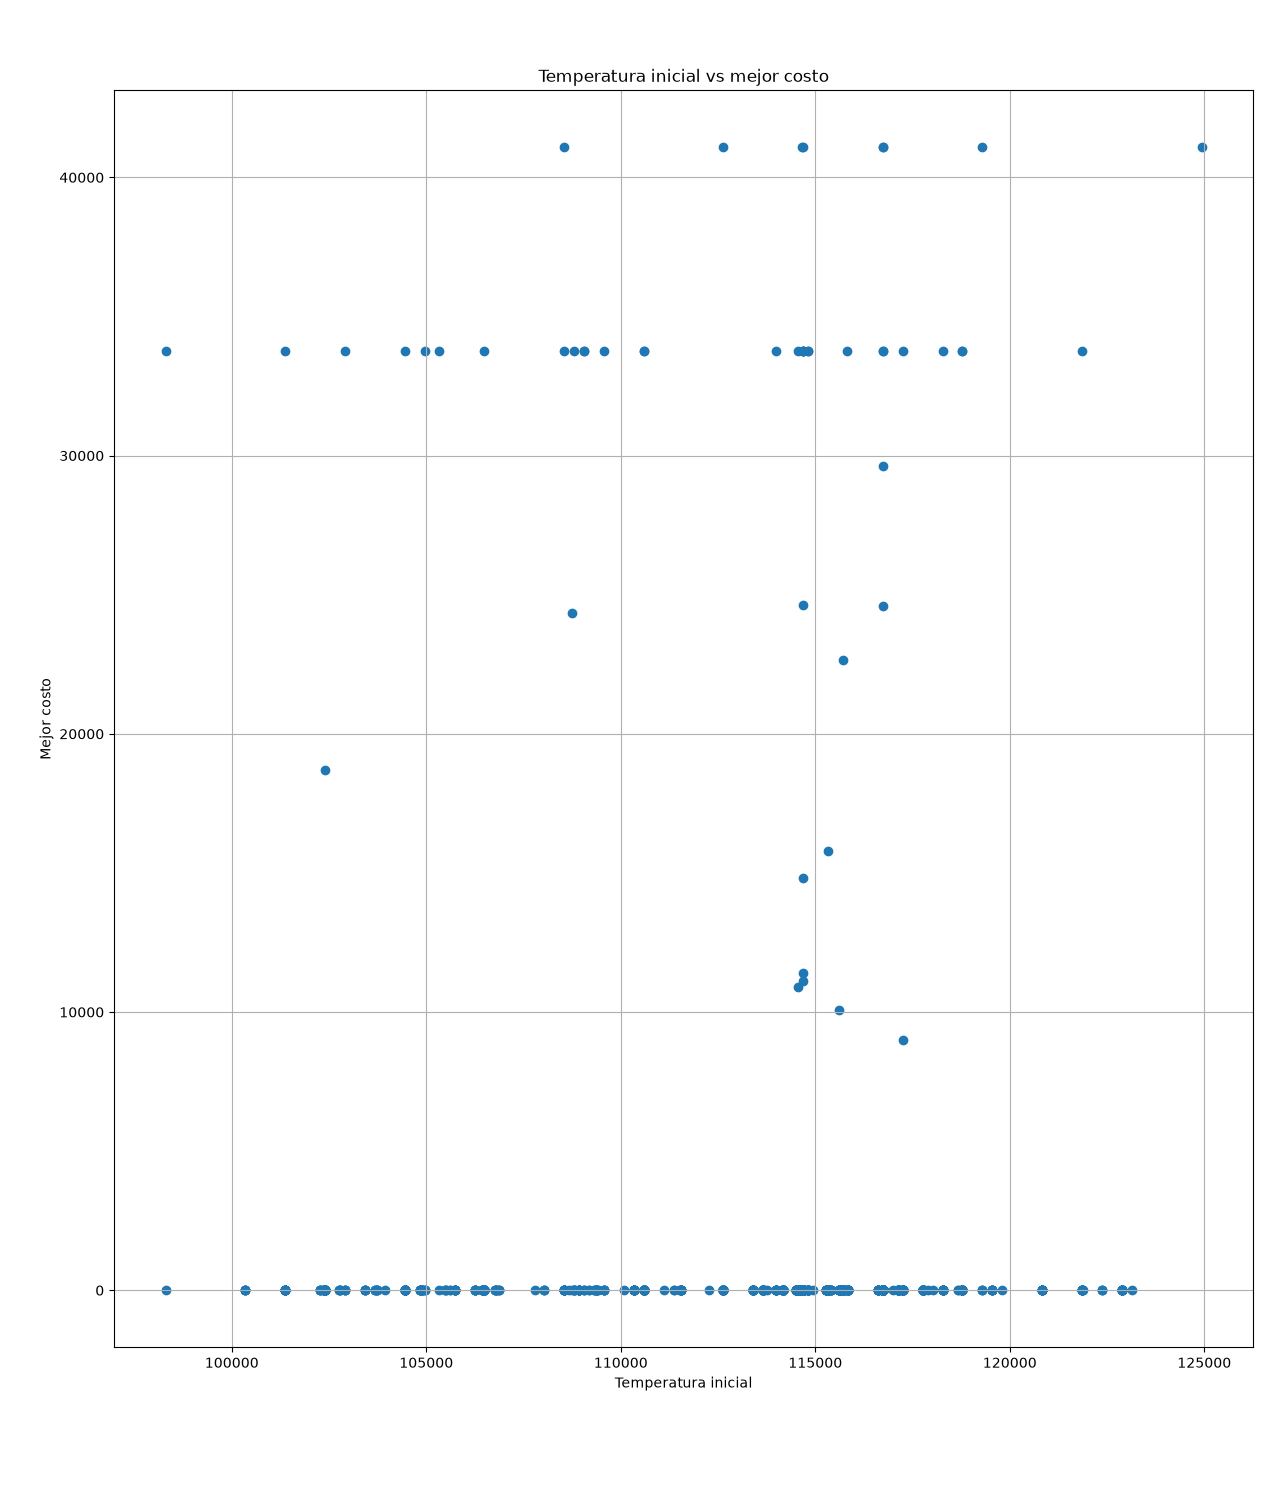
\includegraphics[width=0.48\textwidth]
        {images/MejorCostoTemInicial150.png}
    \caption{Relación del mejor costo con la aceptación objetivo
    y la temperatura inicial calculada.}
    \label{fig:150-aceptacion-temperatura}
\end{figure}
\\\\
Estas gráficas describen las configuraciones efectivamente evaluadas.
La mayor concentración de puntos en determinados intervalos también
depende del mecanismo adaptativo de generación de parámetros.
Por tanto, una región con más observaciones no puede interpretarse
directamente como una región superior.
\\
Además, las configuraciones modificaron varios parámetros y se
evaluaron con distintas semillas. Las gráficas de dispersión no
permiten aislar el efecto causal de un parámetro. La escala dominada
por los costos extremos tampoco permite determinar visualmente
qué configuración es mejor dentro del intervalo de costos bajos.

\subsubsection{Trayectoria de las evaluaciones aceptadas}

La reproducción del récord en modo normal registró 24621160
evaluaciones aceptadas. La Figura~\ref{fig:150-evaluaciones}
muestra una reducción pronunciada de los costos elevados durante
la primera parte de la secuencia.
\begin{figure}[htbp]
    \centering
    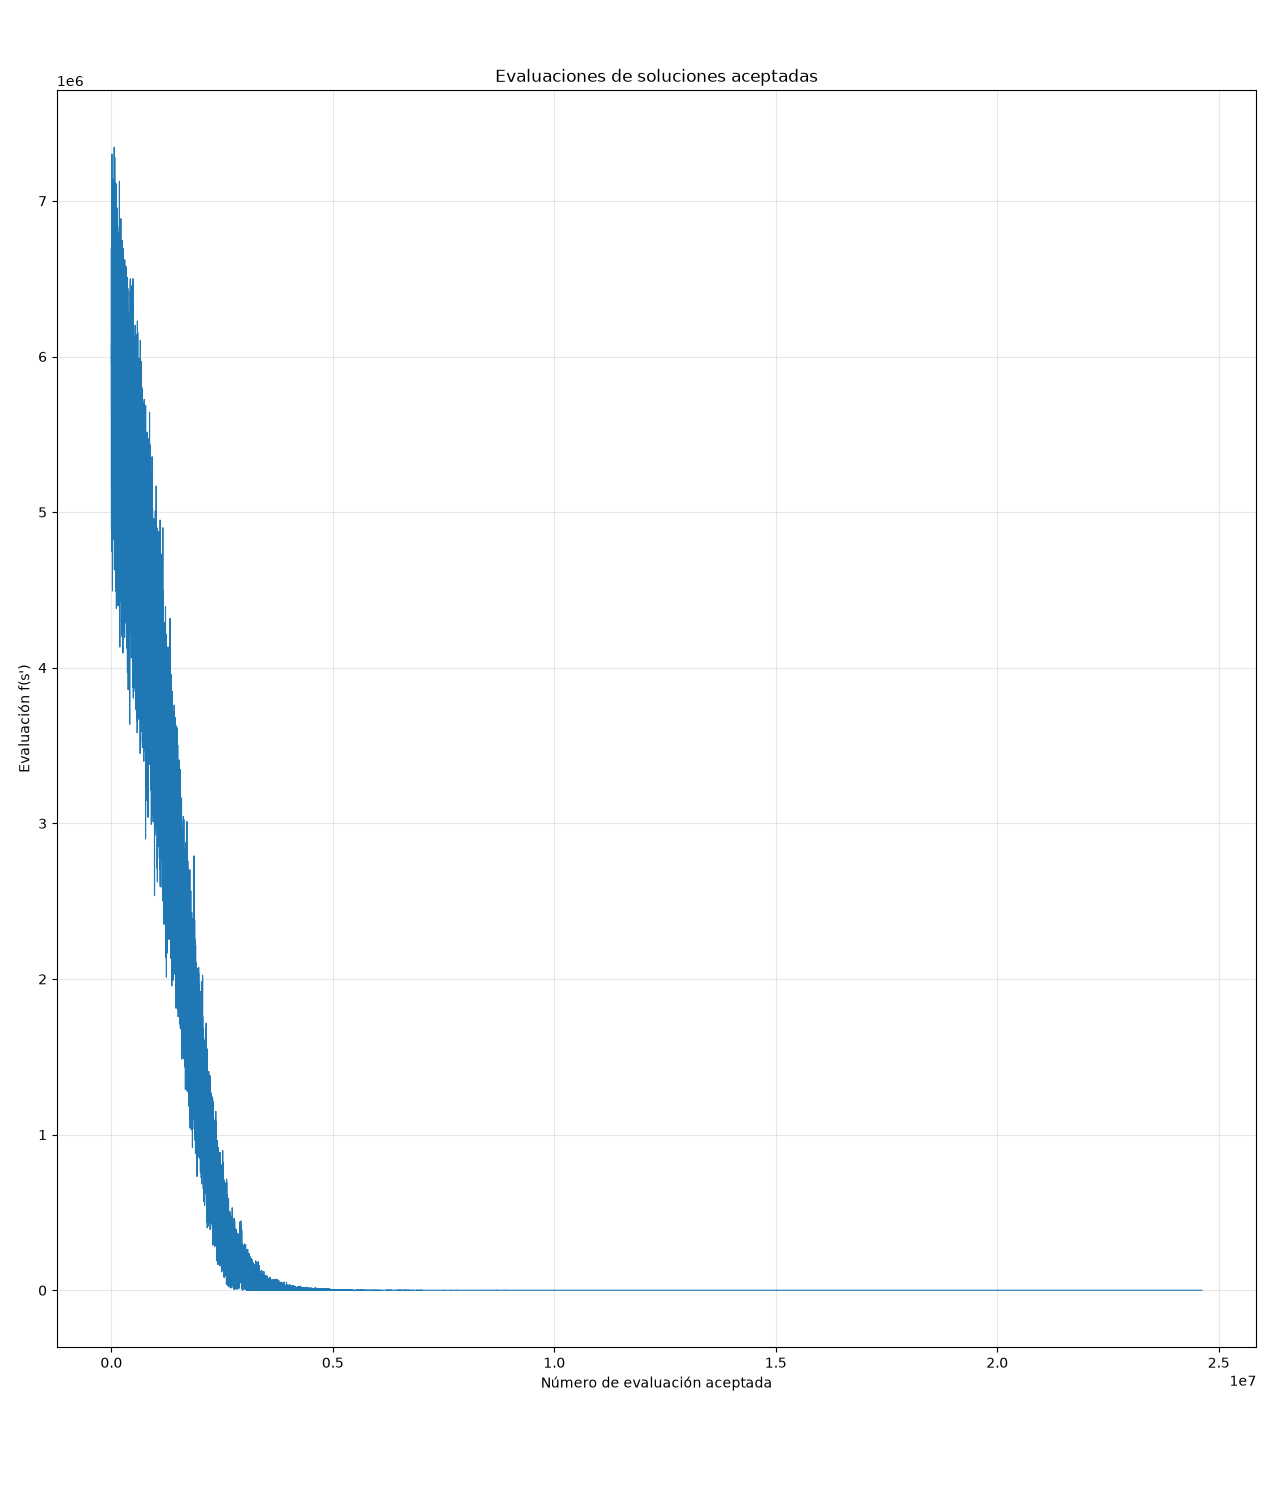
\includegraphics[width=0.76\textwidth]
        {images/EvaluacionesAceptadas150.png}
    \caption{Evaluaciones de las soluciones aceptadas durante
    la reproducción de la mejor corrida de 150 ciudades.
    El eje horizontal cuenta aceptaciones, no tiempo ni intentos.}
    \label{fig:150-evaluaciones}
\end{figure}
\\
En la escala general, los costos pequeños parecen próximos a cero.
Esto no implica que el algoritmo haya alcanzado costo cero ni que
haya dejado de modificar la solución.
\\
El mejor costo apareció por primera vez en la evaluación aceptada
24372819, aproximadamente al $98.99\%$ de la secuencia. Después
se registraron 248341 aceptaciones adicionales sin superar ese
mínimo. Esta ubicación describe la secuencia de aceptaciones;
no permite determinar el porcentaje de tiempo consumido.
\\
La Figura~\ref{fig:150-evaluaciones-zoom} muestra un intervalo muy
reducido del tramo final. Los desplazamientos indicados en los ejes
son necesarios para interpretar correctamente los valores:
las variaciones verticales son del orden de $10^{-6}$ alrededor
de $0.13964$.
\begin{figure}[htbp]
    \centering
    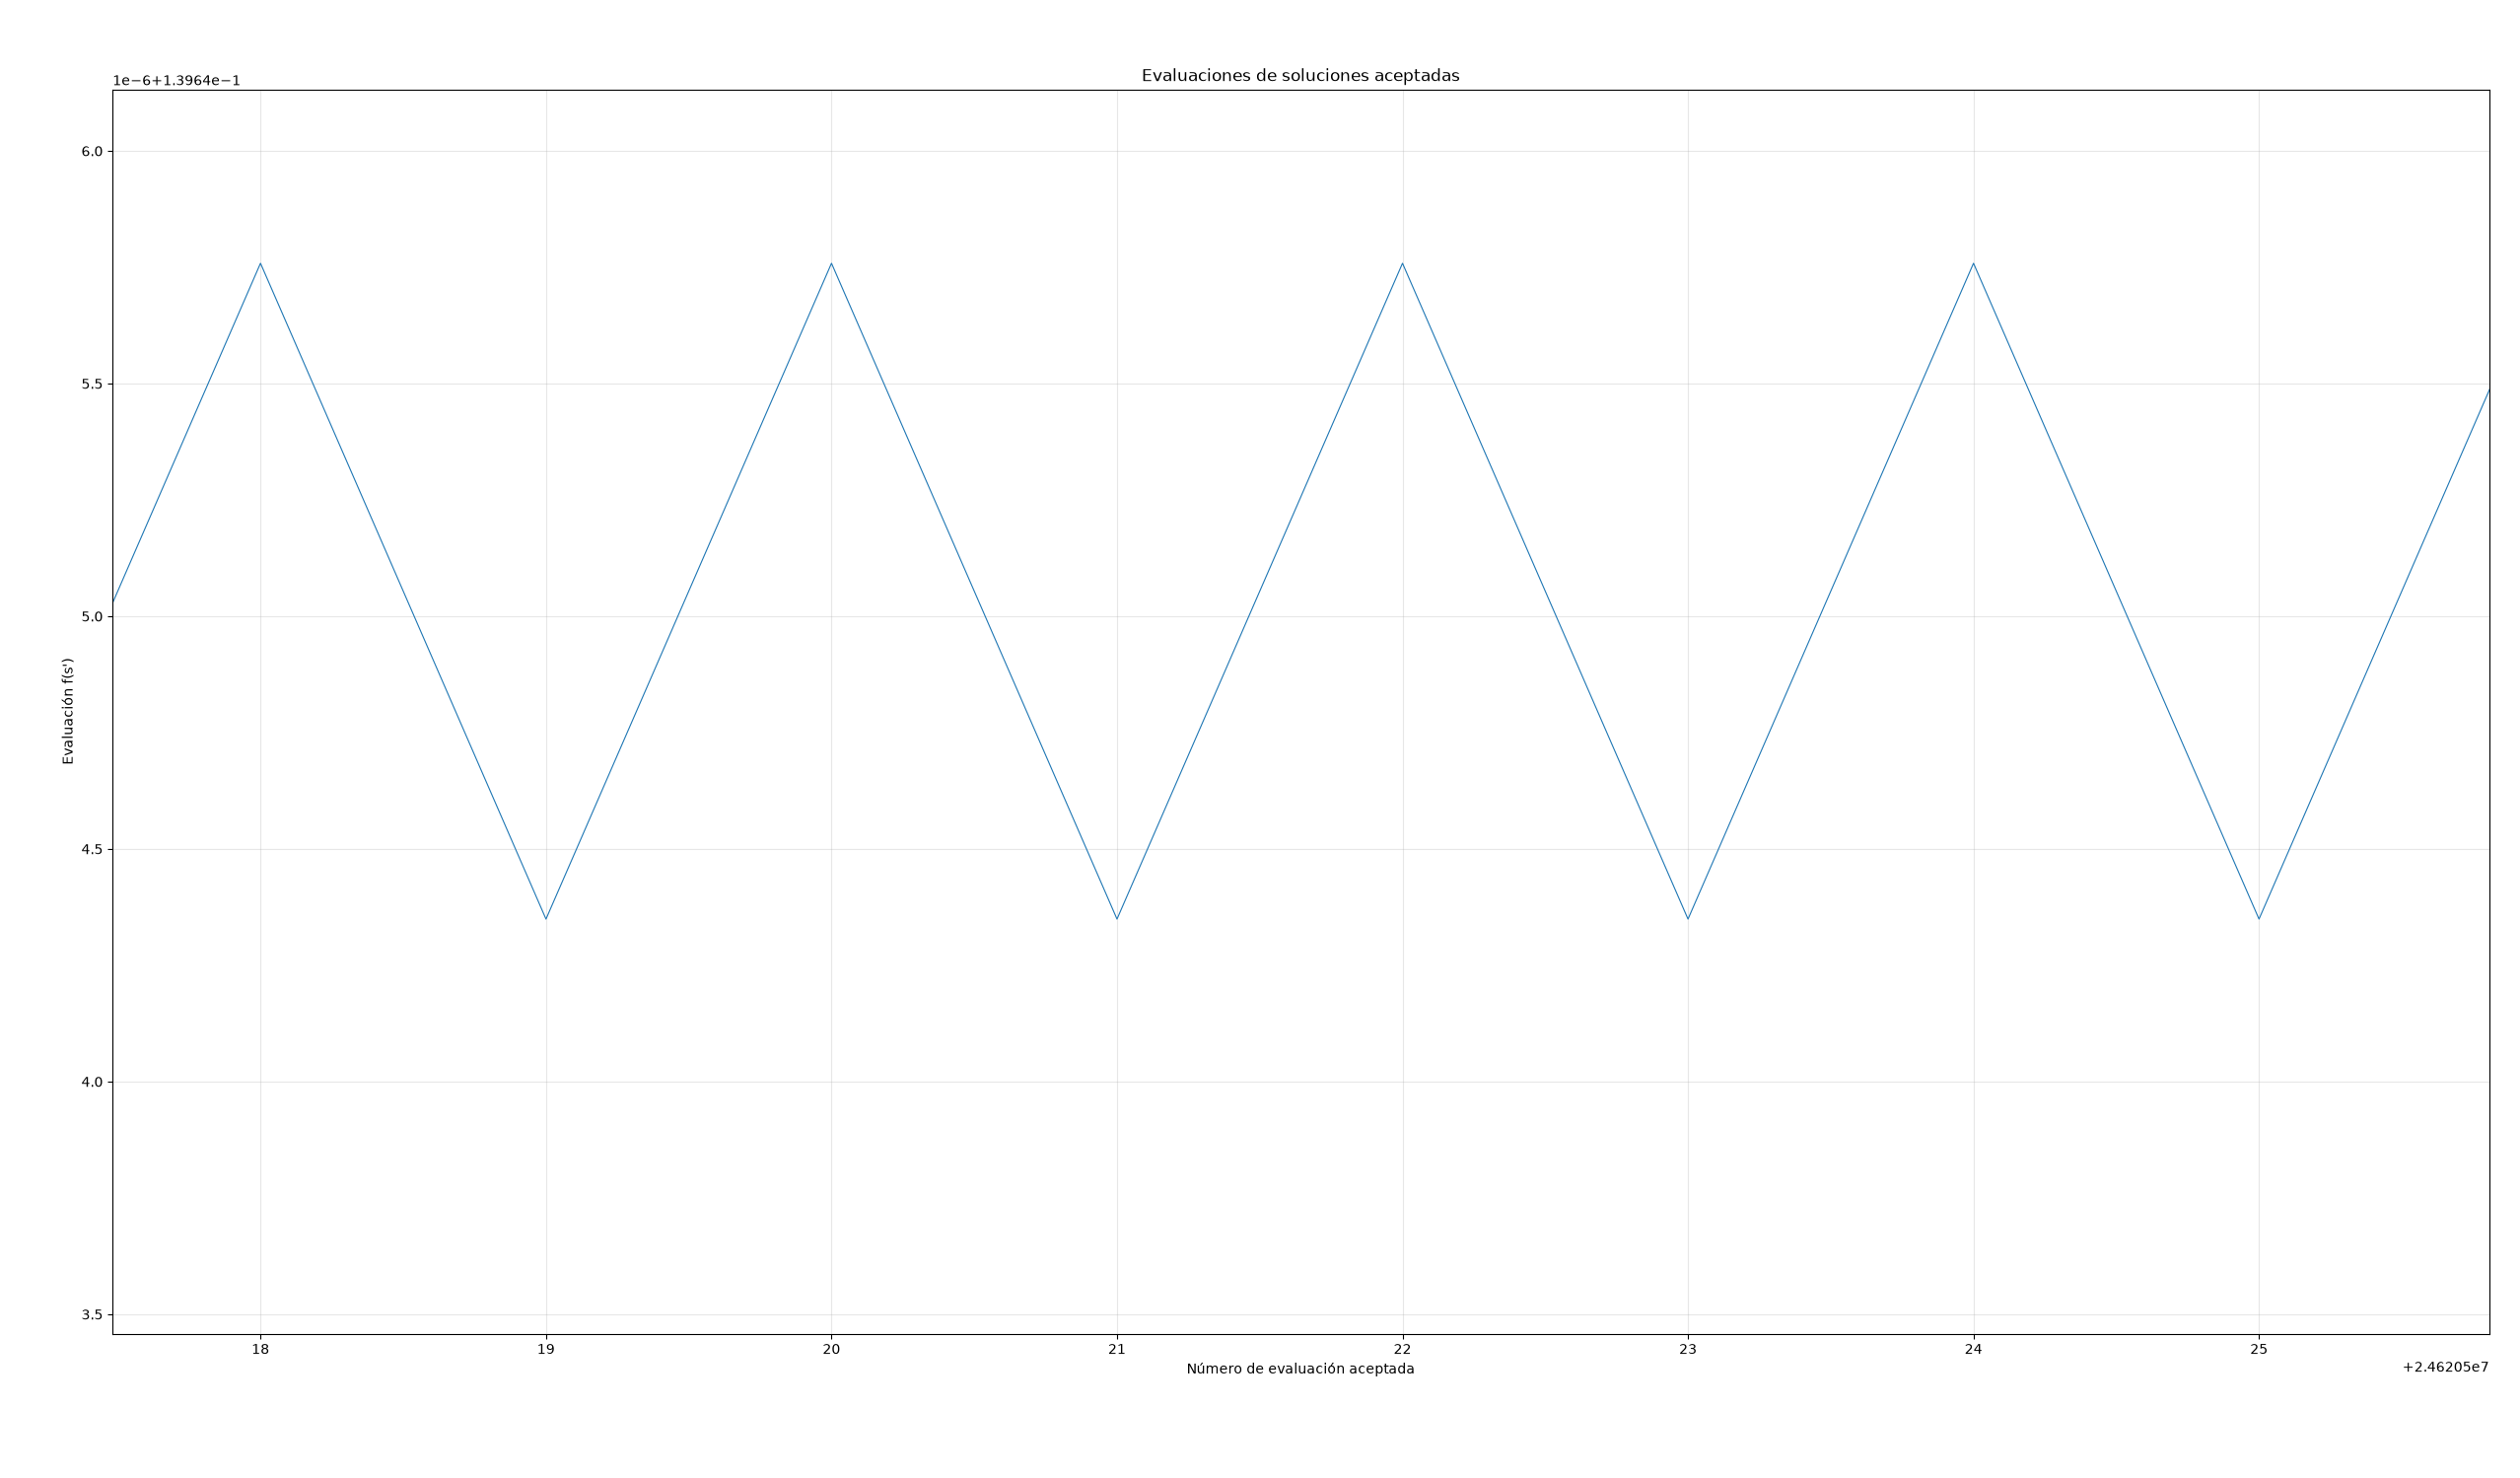
\includegraphics[width=\textwidth]
        {images/EvaluacionesAceptadasFinalZoom150.png}
    \caption{Detalle de un intervalo del tramo final de las
    evaluaciones aceptadas. Se observan pequeñas oscilaciones
    del costo de la solución actual.}
    \label{fig:150-evaluaciones-zoom}
\end{figure}
\\
La corrida terminó con
\[
    f_{\mathrm{final}}=0.13964575855536535,
\]
valor superior al mejor costo guardado. Esto es compatible con
la aceptación de empeoramientos temporales: la solución actual
puede alejarse de la mejor solución visitada. La conservación
explícita del mínimo permite devolver esta última.

\subsubsection{Representación geográfica de la mejor ruta}

La Figura~\ref{fig:150-mapa} presenta la mejor ruta encontrada,
con costo normalizado $0.13945992054852843$ y normalizador
\[
    N=7.225987849734029\times10^8.
\]
\begin{figure}[htbp]
    \centering
    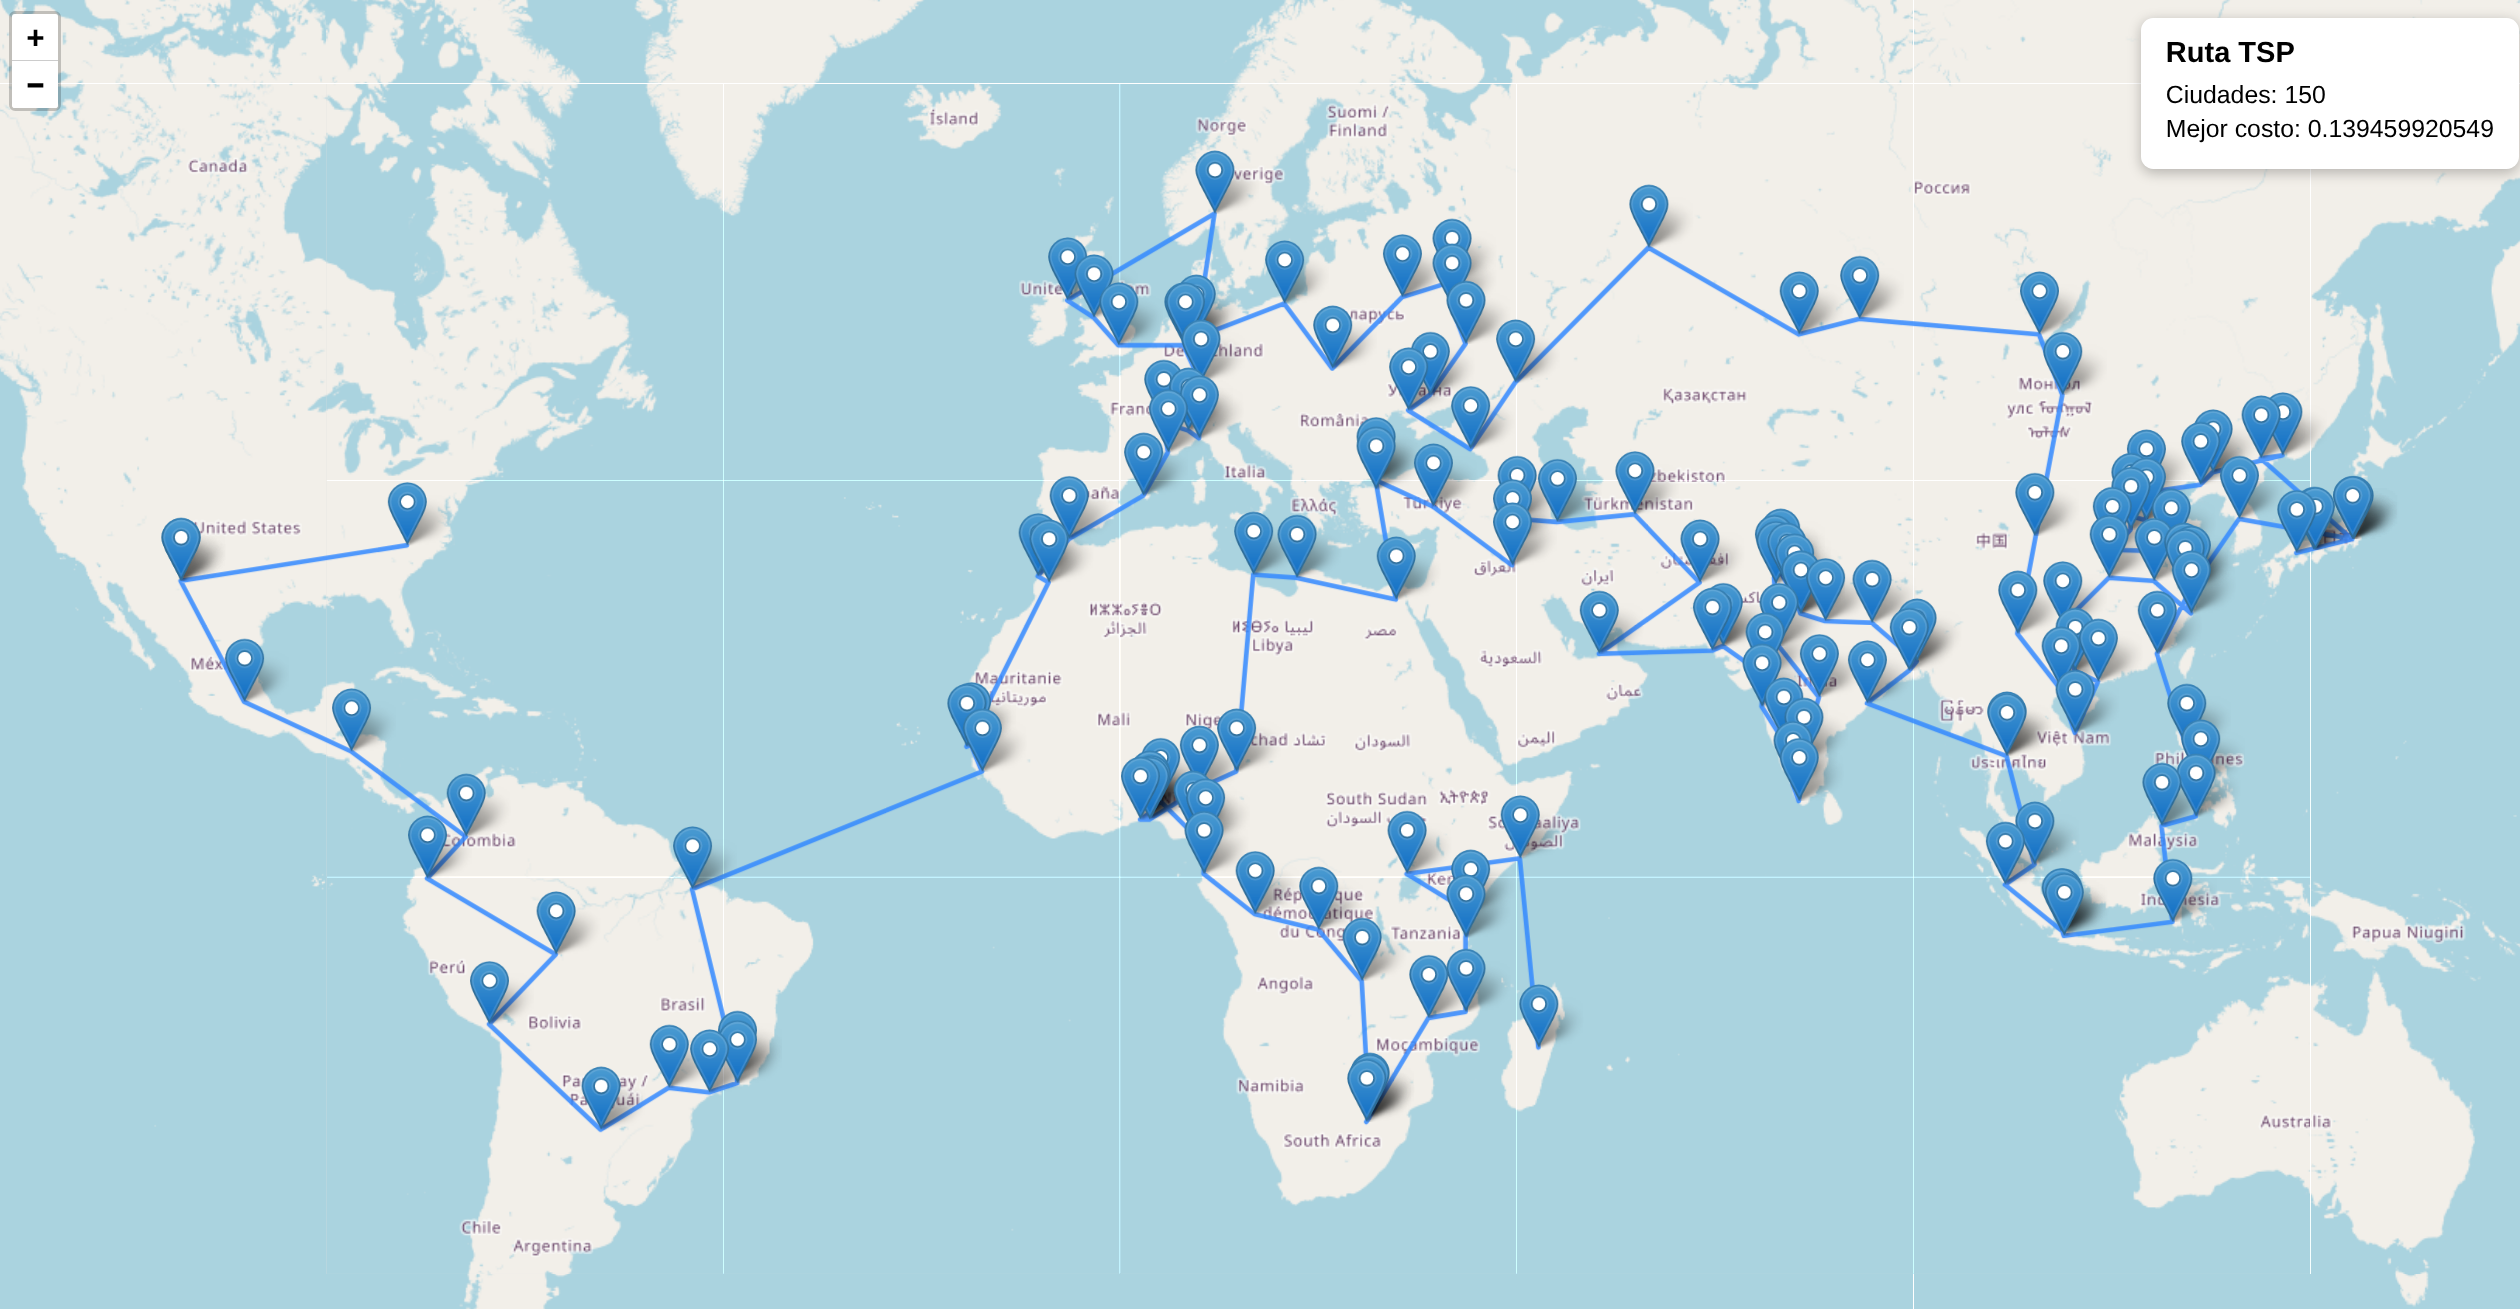
\includegraphics[width=\textwidth]{images/Mapa150150.png}
    \caption{Representación geográfica de la mejor solución
    obtenida mediante Aceptación por Umbrales para 150 ciudades.
    Mapa base de OpenStreetMap.}
    \label{fig:150-mapa}
\end{figure}
\\
Los segmentos unen ciudades consecutivas de la solución. La
visualización facilita inspeccionar el orden del recorrido, pero
no representa necesariamente trayectos por carretera ni sustituye
la evaluación de los pesos de la instancia.
\\
De acuerdo con la variante implementada, el costo suma las
149 conexiones entre ciudades consecutivas de la permutación,
sin añadir una conexión de regreso desde la última ciudad a
la primera.

\subsubsection{Resultados de los experimentos complementarios}

Los experimentos A, B y C completaron 216 corridas adicionales.
La Tabla~\ref{tab:150-complementarios} presenta sus resultados.
\begin{table}[htbp]
    \centering
    \small
    \begin{tabular}{lrrr}
        \hline
        Medida & A & B & C \\
        \hline
        Corridas & 72 & 72 & 72 \\
        Mejor costo
            & $0.1394599205$ & $0.1400323471$ & $0.1410819573$ \\
        Mediana
            & $0.1620323748$ & $0.1629528118$ & $0.1569444904$ \\
        Costos mayores o iguales que $1$
            & 1 & 2 & 0 \\
        \hline
    \end{tabular}
    \caption{Resultados de tres experimentos complementarios.
    A y B variaron las semillas con parámetros fijos; C varió
    los parámetros con la semilla base 123.}
    \label{tab:150-complementarios}
\end{table}
\\
$A$ reprodujo el récord con la semilla base 123. $B$ reprodujo el
resultado $0.1400323471$ con la semilla base 789. Las semillas
adicionales no superaron estos valores.
\\
$C$ evaluó 67 configuraciones distintas y realizó cinco repeticiones
de campeones entre generaciones. Su mejor resultado apareció en
la generación 1. Aunque su mediana fue menor que las de $A$ y $B$,
los diseños no son equivalentes: $C$ no evaluó la robustez de cada
configuración frente a múltiples semillas.
\\
También se realizaron pruebas manuales en modo normal. La
reducción de la temperatura final a $3\times10^{-7}$ añadió
niveles de enfriamiento a las corridas de referencia $A$ y $B$,
pero no mejoró sus respectivos récords. En $B$, modificar el
factor de enfriamiento a $0.9921$ produjo $0.1463053572$,
mientras que aumentar el lote a 5600, manteniendo el máximo
de intentos, produjo $0.1639559701$.
\\
Estos resultados muestran que cambios pequeños en los parámetros
pueden alterar considerablemente la trayectoria de búsqueda.
No existe, a partir de estas pruebas, evidencia de una relación
monótona entre incrementar un parámetro y mejorar el costo.

\subsubsection{Alcance de los resultados}

El resultado principal de Aceptación por Umbrales fue reproducible,
pero apareció de forma excepcional en el experimento original.
Las búsquedas complementarias no lograron superar
$0.13945992054852843$.
\\\\
La interrupción del experimento original, el muestreo adaptativo
de parámetros y la repetición de configuraciones campeonas limitan
la interpretación estadística de los registros. Las corridas no
constituyen una muestra independiente y uniforme del espacio
de configuraciones.
\\\\
Finalmente, el menor costo observado no es una prueba de
optimalidad global ni de optimalidad local. Los resultados
documentan el desempeño del sistema bajo los parámetros,
semillas y presupuestos ejecutados.

\section{Conclusiones y Comentarios}

Los métodos heurísticos de optimización combinatoria, en particular
los basados en búsqueda local, ofrecen una manera práctica de abordar
problemas difíciles, como el Problema del Agente Viajero. En ocasiones,
utilizarlos puede sentirse como lanzar dardos en la oscuridad; sin
embargo, la función objetivo, el vecindario y el criterio de aceptación
permiten orientar los lanzamientos y medir qué tan cerca estamos de
nuestro propósito. Su utilidad consiste en encontrar soluciones de
buena calidad cuando obtener y certificar una solución óptima resulta
computacionalmente costoso.
\\\\
Esta utilidad viene acompañada de cierta frustración: encontrar una
buena solución no elimina la sospecha de que podría existir otra
mejor. En este proyecto, esa sospecha motivó numerosas ejecuciones,
ajustes de parámetros y revisiones de resultados. Aprendí que una
corrida más larga, una temperatura distinta o una semilla nueva no
necesariamente producen una mejora. El algoritmo, por desgracia, no
concede puntos adicionales por insistencia.
\\\\
El proyecto también representó un ejercicio importante de programación
y diseño de sistemas. Además de implementar la heurística, fue
necesario organizar el acceso a los datos, representar las soluciones,
controlar la precisión numérica, realizar pruebas y generar reportes.
Considero que este trabajo refleja una necesidad frecuente en
aplicaciones reales: construir herramientas que permitan experimentar,
reproducir resultados y comprender sus limitaciones.
\\\\
En lo personal, me hubiera gustado obtener mejores resultados,
especialmente para la instancia de 150 ciudades, cuyo mejor costo
registrado mediante Aceptación por Umbrales fue
$0.13945992054852843$. Después de tantos intentos, fue difícil no
sentir que la suerte estaba colaborando más con otros experimentos
que con el mío. Sin embargo, atribuir el resultado únicamente al azar
sería insuficiente: también influyen el vecindario, los parámetros,
la solución inicial y la forma de distribuir el esfuerzo experimental.
Disponer de más tiempo habría permitido explorar otras alternativas,
pero no habría garantizado una solución mejor.
\\\\
Aun con estas limitaciones, los resultados cuentan con registros,
métricas y reproducciones que permiten evaluar el desempeño del
sistema. La distinción entre el mejor resultado individual y el
comportamiento promedio fue especialmente importante: una
configuración capaz de producir una solución sobresaliente con una
semilla no necesariamente ofrece buenos resultados con las demás.
Por ello, la calidad del sistema debe valorarse tanto por las
soluciones obtenidas como por la posibilidad de analizarlas y
reproducirlas.
\\\\
Finalmente, la idea de aceptar empeoramientos temporales para buscar
mejores soluciones me parece una de las enseñanzas más interesantes
del proyecto. Aceptación por Umbrales retoma esta idea del recocido
simulado, inspirado en el proceso físico de recocido de los metales,
y la expresa mediante una regla de aceptación sencilla. Aunque
alejarse de una buena solución puede parecer contradictorio, hacerlo
de manera controlada permite explorar alternativas que una búsqueda
exclusivamente descendente no visitaría. En este caso, no todos los
desvíos llevaron a una mejora, pero sí permitieron comprender mejor
el problema y los límites de la estrategia implementada.

\clearpage
% ==========================================================
% Bibliografía
% ==========================================================

\clearpage
\renewcommand{\refname}{Bibliografía}

\begin{thebibliography}{9}

\bibitem{lawler1985tsp}
Lawler, E.~L., Lenstra, J.~K., Rinnooy Kan, A.~H.~G.
y Shmoys, D.~B. (eds.).
\textit{The Traveling Salesman Problem:
A Guided Tour of Combinatorial Optimization}.
John Wiley \& Sons, 1985.

\bibitem{garey1979computers}
Garey, M.~R. y Johnson, D.~S.
\textit{Computers and Intractability:
A Guide to the Theory of NP-Completeness}.
W.~H. Freeman and Company, 1979.

\bibitem{dueck1990threshold}
Dueck, G. y Scheuer, T.
``Threshold accepting: A general purpose optimization
algorithm appearing superior to simulated annealing''.
\textit{Journal of Computational Physics},
vol.~90, núm.~1, pp.~161--175, 1990.
\href{https://doi.org/10.1016/0021-9991(90)90201-B}
{doi:10.1016/0021-9991(90)90201-B}.

\bibitem{pelaezTSP}
Peláez Valdés, Canek.
\textit{El Problema del Agente Viajero}.
Capítulo 4, apuntes de clase del Seminario de Heurísticas
de Optimización Combinatoria.
Facultad de Ciencias, Universidad Nacional Autónoma de México,
s.~f.
Material docente no publicado, distribuido por el profesor
en formato PDF.

\bibitem{pelaezUmbrales}
Peláez Valdés, Canek.
\textit{Aceptación por Umbrales}.
Capítulo 7, apuntes de clase del Seminario de Heurísticas
de Optimización Combinatoria.
Facultad de Ciencias, Universidad Nacional Autónoma de México,
s.~f.
Material docente no publicado, distribuido por el profesor
en formato PDF.

\end{thebibliography}

\end{document}